%=================================================================
% IduEdu — Smart Cities (MDPI) manuscript
% Special Issue: Sustainable Mobility in Smart Cities: Advancing
%                Accessibility, Efficiency, and Equity
%=================================================================
\documentclass[smartcities,article,submit,moreauthors]{Definitions/mdpi}

%=================================================================
\firstpage{1}
\makeatletter
\setcounter{page}{\@firstpage}
\makeatother
\pubvolume{1}
\issuenum{1}
\articlenumber{0}
\pubyear{2026}
\copyrightyear{2026}
\datereceived{ }
\daterevised{ }
\dateaccepted{ }
\datepublished{ }

%=================================================================

\usepackage[T2A,T1]{fontenc}
\newcommand{\xmark}{$\times$}
\newcommand{\pmark}{(\checkmark)}

\newcommand{\cyr}[1]{{\fontencoding{T2A}\selectfont #1}}

\newcommand{\STYLE}[1]{\textcolor{magenta}{\textbf{[STYLE: {\fontencoding{T2A}\selectfont #1}]}}}

%=================================================================

\Title{IduEdu: An Open-Source GeoDataFrame-Native Infrastructure for Multimodal Accessibility Analysis and Rapid Scenario Screening in Smart Cities}

\newcommand{\orcidauthorA}{0009-0002-7881-1543}
\newcommand{\orcidauthorB}{0000-0002-6382-5259}

\Author{Danila Oleynikov $^{1,}$*\orcidA{} and Natalia Chichkova $^{1}$\orcidB{}}

\AuthorNames{Danila Oleynikov and Natalia Chichkova}

\address{%
    $^{1}$ \quad ITMO University, Saint Petersburg, Russia; ddonnyy@itmo.ru (D.O.);
    nachichkova@niuitmo.ru (N.C.)}

\corres{Correspondence: ddonnyy@itmo.ru}

%=================================================================

\abstract{Smart-city planning requires repeatable, city-scale assessment of multimodal accessibility,
    yet open-data workflows remain limited by fragmented tooling and the computational cost of building,
    storing and repeatedly re-computing explicit urban network graphs.
    This paper presents IduEdu, an open-source Python library that provides a GeoDataFrame-native urban
    graph infrastructure, so spatial editing and routing operate on the same representation.
    IduEdu builds walking, driving and static public transport graphs directly from OpenStreetMap without
    requiring GTFS, and exposes scalable routing primitives.
    Across six large cities, IduEdu builds street graphs $3.3$--$9.3\times$ faster than OSMnx, the de
    facto standard open-source tool for urban street-network analysis, with an order-of-magnitude
    smaller in-memory representation, and matches or exceeds optimized C/C++ graph backends on
    batch accessibility workloads.
    In a city-scale case study of Saint Petersburg (83{,}510 residential buildings, 911 schools), adding
    public transport to the walk-only network raises the mean number of schools reachable within 30~min
    from 9.5 to 23.5, and a route-by-route screening of the city's 635 transit routes
    shows this gain to rest on a small critical backbone of the network.}

% Keywords — 3–10
\keyword{smart cities; urban accessibility; multimodal networks; OpenStreetMap; public transport; scenario analysis; origin--destination matrices; open-source software}

%=================================================================
\begin{document}


    \section{Introduction}
    \label{sec:introduction}

    Smart cities increasingly depend on the ability to evaluate urban mobility and service accessibility
    in a repeatable, data-driven way.
    Decisions about where to densify housing, which public transport (PT) services to protect or extend,
    and how resilient a network is to disruption all require quantitative evidence about who can reach
    which opportunities, by which modes, and how this picture changes under alternative
    scenarios~\cite{zini2024competitiveness,gumina2026mapping}.
    Such assessments are most valuable when they can be re-run---for a new neighborhood, an updated
    network, or a hypothetical intervention---rather than produced once as a static study.

    Open geospatial data, and OpenStreetMap (OSM)~\cite{arsanjani2015osm} in particular, make this kind
    of analysis transferable across cities, including cities where official transit feeds, smart-card
    records or survey data are unavailable.
    In practice, however, three barriers limit open-data mobility analytics at the city scale.
    First, the required transport data---street geometry and attributes, public transport routes and
    stop infrastructure, and, where available, service schedules---and the tooling around them are
    fragmented: street extraction, transit modeling and accessibility computation live in different
    libraries with incompatible representations.
    Second, constructing and storing explicit multimodal networks for a large city is expensive in both
    time and memory~\cite{staudt2016networkit,benchmark_graphtools}, a cost we quantify in
    Section~\ref{subsec:res-build}.
    Third, and most restrictive for planning applications, comparing many planning or disruption
    scenarios requires re-computing accessibility over and over, which multiplies the first two costs.

    Existing open-source solutions each cover a part of the chain from network extraction through
    graph construction to accessibility computation.
    High-performance routing engines and simulation frameworks answer individual queries quickly but
    hide the network behind a service API~\cite{osrm,otp,graphhopper,valhalla}; accessibility frameworks
    provide indicators but depend on GTFS feeds and external routing
    services~\cite{blanchard2017urbanaccess,foti2014pandana,gumina2026mapping}; graph-extraction
    libraries produce explicit street networks but neither public transport graphs nor scalable batch
    computations~\cite{boeing2025osmnx,pyrosm_docs}.

    Between these families lies an infrastructural gap: there is no widely adopted layer that couples an
    \emph{explicit, modifiable} multimodal graph with \emph{fast, repeatable} accessibility computation
    in a standard geospatial data model.

    Recent smart-mobility frameworks demonstrate compelling applied
    scenarios~\cite{gogousou2026mobilityoracle,shulajkovska2024framework,salanovagrau2026pollution}, but
    they typically do not examine the computational cost of repeatedly building, storing and
    re-evaluating explicit multimodal city graphs.

    What remains underexplored is an open, OSM-based pipeline that simultaneously (i) yields a spatial
    graph that is directly accessible and modifiable by the analyst, (ii) builds a static PT network
    without requiring GTFS, (iii) scales to massive origin--destination (OD) workloads, and (iv)
    quantifiably reduces the cost of repeated scenario analytics---while remaining compatible with the
    GeoPandas workflow and with user-defined algorithms.

    We therefore ask four research questions.
    The first three concern the infrastructure itself---whether such a representation can be built from
    open data, what it costs, and whether that cost admits repeated city-scale analysis---while the
    fourth tests the premise underlying them: whether an explicit multimodal network changes the
    analytical conclusions at all, relative to the walk-only networks that current open-source tools
    already provide.
    \begin{itemize}
        \item \textbf{RQ1.} Can a single OSM-based pipeline construct an explicit and compact
        multimodal representation of an urban network without requiring GTFS?
        \item \textbf{RQ2.} To what extent does a unified tabular representation reduce end-to-end pipeline construction
        time and graph-representation size compared with the widespread OSMnx/NetworkX stack and specialized graph backends?
        \item \textbf{RQ3.} Does the resulting efficiency allow city-scale accessibility assessment and
        repeated transport scenario screening within practically useful time?
        \item \textbf{RQ4.} Does a multimodal network affect the results of a city-scale
        service-accessibility assessment (here, schools) relative to the walk-only network that current
        open-source tools provide, and how strongly does this effect depend on individual transport
        modes and routes?

    \end{itemize}

    We answer these questions with IduEdu~\cite{iduedu_docs}, an open-source Python library built
    around \texttt{UrbanGraph}, a GeoDataFrame-native graph model.
    The contributions are: (i) an open-source, GeoDataFrame-native urban graph model in which editable spatial tables
    and the sparse computational representation are synchronized views of the same network; (ii) a pipeline for
    constructing static PT and multimodal graphs directly from OSM without mandatory GTFS; (iii) scalable nearest-source
    and batch-OD routing primitives combined with cache-aware graph reuse and table-level scenario editing;
    (iv) a reproducible evaluation of graph construction, representation size, routing scalability and per-scenario
    runtime against relevant graph stacks; and (v) a city-scale school-accessibility case study that maps multimodal
    accessibility gains and evaluates leave-one-route-out criticality across 635 PT routes together with
    service-degradation scenarios.
    To demonstrate downstream composability, ObjectNat~2.0~\cite{objectnat_docs}---an open-source
    library for urban accessibility and service-provision indicators---consumes \texttt{UrbanGraph}
    directly to construct isochrone and coverage geometries, while scenario logic is expressed
    through ordinary GeoPandas table operations and can likewise be replaced or extended by user-defined algorithms.

    Integrated into a smart-city analytical stack, these properties bear directly on the recurring
    planning tasks reviewed in Section~\ref{subsec:rw-tasks}: monitoring service accessibility,
    comparing it across modes and population groups, ranking the transit elements a city most depends
    on, and evaluating proposed interventions before they are committed.
    An OSM-derived transit layer makes such analysis possible where no transit feed is maintained,
    while an explicit and editable graph lets these tasks share one network at a cost of seconds per
    scenario.

    The remainder of the paper reviews related tools, defines the graph model and experimental protocol,
    reports the construction, routing, accessibility and scenario results, and closes with their
    implications, limitations and conclusions.

%%%%%%%%%%%%%%%%%%%%%%%%%%%%%%%%%%%%%%%%%%


    \section{Related Work}
    \label{sec:related-work}

    \subsection{Mobility Management Tasks in Smart Cities and Their Network Requirements}
    \label{subsec:rw-tasks}

    Smart-city mobility management is not a single problem but a set of recurring analytical tasks,
    each with an established geospatial modelling practice.
    Five of them account for most of the network-based literature relevant to this paper.

    \begin{itemize}
        \item \textbf{T1. Service accessibility and proximity planning.}
        How many opportunities---shops, schools, clinics---residents can reach within a travel-time
        budget, the question underlying the ``15-minute city'' agenda now embedded in municipal
        policy. The conventional model is a set of isochrones or cumulative-opportunity counts
        computed on a pedestrian network. Its limits are empirically documented: from GPS traces of
        40 million devices, Abbiasov et al.~\cite{abbiasov2024fifteenmin} find that the median US
        resident makes only 14\% of consumption trips within a 15-minute walk of home, so an
        assessment confined to the walk network describes a small fraction of realized access.

        \item \textbf{T2. Accessibility of social facilities and territorial equity.}
        Whether disadvantaged or car-free populations can reach healthcare and education, typically
        modelled with two-step floating catchment or cumulative-opportunity measures computed over
        public transport. Gumina et al.~\cite{gumina2026mapping} contrast car and PT travel times to
        education and healthcare in the Lazio region and weight the result by population; Zini et
        al.~\cite{zini2024competitiveness} frame the same contrast as PT competitiveness with equity
        implications for Rome and Turin. Bellantuono et al.~\cite{bellantuono2025rome} motivate the
        task explicitly by transport poverty---residents without a car depend on transit alone for
        medical access.

        \item \textbf{T3. Network resilience and criticality screening.}
        Which elements of the network carry the structural load and what happens when they fail.
        Palk et al.~\cite{palk2026robustness} systematically review robustness assessment of public
        transport networks and show that the choice of graph representation is itself a trade-off
        between complexity reduction and information preservation that conditions the robustness
        conclusions drawn from it. Bergantino et al.~\cite{bergantino2024resilience} review the
        empirical side of this literature. Bellantuono et al.~\cite{bellantuono2025rome} instantiate
        the task for a service: they remove high-centrality transit nodes and measure the induced
        change in travel time to healthcare facilities, finding that accessibility resilience is
        governed by network redundancy. Methodologically the task \emph{is} a sequence of network
        modifications, each followed by re-computation.

        \item \textbf{T4. Multimodal integration and land-use coupling.}
        How modes function together and how the resulting accessibility relates to land use. Ladin et
        al.~\cite{ladin2025review} review modelling approaches for multimodal systems across
        optimization, travel behaviour and resilience, and identify data limitations and
        computational complexity as recurring constraints on scalability. Gu and
        Dou~\cite{gu2026multilayer} state the gap directly---accessibility has largely been assessed
        within single transport modes, with limited attention to the integrated functioning of
        multimodal systems---and address it with a multilayer network model over 7826 urban grids in
        Shanghai, in which peripheral zones show fragmented connectivity that single-mode analysis
        does not expose.

        \item \textbf{T5. Policy and scenario evaluation.}
        Comparing a baseline against candidate interventions. Shulajkovska et
        al.~\cite{shulajkovska2024framework} compute formalized KPIs for baseline and policy scenarios
        across four cities using MATSim simulations; Salanova Grau et
        al.~\cite{salanovagrau2026pollution} compare baseline and pollution-aware pedestrian routes
        over 3000 OD pairs, quantifying an ${\approx}4\%$ exposure reduction for an ${\approx}3\%$
        detour; Liyanage et al.~\cite{liyanage2025ondemand} evaluate on-demand transit with a hybrid
        simulation calibrated on 225,000 smart-card trips. In the framework closest to ours, The
        Mobility Oracle~\cite{gogousou2026mobilityoracle}, what-if scenarios such as a street closure
        are expressed as modifications of a multimodal graph followed by re-computation of the same OD
        relations.
    \end{itemize}

    Two requirements recur across these tasks.
    First, most of them cannot be answered on a single-mode network: T1 and T2 compare walking against
    transit-based access, T3 asks what a transit element contributes over the alternatives that remain
    once it is gone, and T4 makes modal integration the object of study itself.
    What they require is an explicit \emph{multimodal} graph in which walking, transit services and the
    transfers between them are represented in one structure---and, for T3 and T5, one that can be
    modified.
    Second, none of these tasks is a single computation: proximity targets are monitored over time,
    criticality is screened element by element, and scenarios are compared in series.
    The cost of constructing such a network and re-computing over it therefore bounds which questions
    can be asked at all---a constraint the reviews above name~\cite{ladin2025review} but do not
    quantify.
    The remainder of this section examines how such graphs are built and computed today.

    \subsection{Constructing Urban Network Graphs from Open Data}
    \label{subsec:rw-construction}

    Street-network extraction from OSM is mature.
    \textbf{OSMnx}~\cite{boeing2025osmnx} is the most widely used Python tool for extracting and
    analyzing street networks from OSM, applied across a broad range of urban
    studies~\cite{coutrot2022,nilsson2019,feng2020,liao2020}.
    It automates network download via the Overpass API~\cite{overpass_api} and produces a directed
    \texttt{networkx.MultiDiGraph}~\cite{hagberg2008networkx}, with mature support for visualization,
    graph simplification and basic street-network analysis.
    \textbf{Pyrosm}~\cite{pyrosm_docs} offers an alternative based on local OSM PBF extracts; its Cython
    implementation is efficient for city- to country-scale processing.
    Both target static street networks and neither constructs public transport or multimodal graphs.

    Extending construction to public transport is where the tooling thins out, and where a common
    dependency appears.
    \textbf{UrbanAccess}~\cite{blanchard2017urbanaccess} and the companion library
    \textbf{OSMnet}~\cite{osmnet_github}, parts of the Urban Data Science Toolkit, construct an
    integrated pedestrian--transit representation from OSM and General Transit Feed Specification
    (GTFS) data~\cite{gtfs_spec}: UrbanAccess processes GTFS feeds while OSMnet extracts the walking
    network.
    The result is exposed as \texttt{pandas} DataFrames~\cite{mckinney2010pandas} and is primarily
    intended for accessibility computation in \texttt{Pandana}~\cite{foti2014pandana}.
    For a selected service period, UrbanAccess converts scheduled travel times into fixed edge costs
    and estimates waiting as half the average headway.
    Its GTFS ingestion mechanism relies on the GTFS Data Exchange catalog, unmaintained since 2016,
    which renders many feeds unavailable; the latest release (0.2.2) dates to 2020.
    \textbf{Peartree}~\cite{peartree_github} converts GTFS feeds into a static route-and-stop PT graph
    in NetworkX format (with OSMnx suggested for the walk layer); it implements no routing algorithms
    of its own, and its latest release (0.6.4) dates to 2021.
    \textbf{NxTransit}~\cite{nxtransit} combines GTFS feeds with OSM street data into a multimodal
    NetworkX graph and adds time-dependent shortest paths, travel-time matrices and service-area
    analysis; its repository was archived in January 2025.
    \textbf{city2graph}~\cite{city2graph} converts OSM, Overture, GTFS and shared-mobility feeds into
    graph representations that interoperate between GeoDataFrames, NetworkX and PyTorch Geometric;
    it targets graph neural networks and feature preparation rather than routing, and does not compute
    travel times or accessibility itself.

    Two properties are shared by all four transit-capable builders.
    Each requires a GTFS feed for the transit layer, which restricts them to cities that publish and
    maintain one---a substantial limitation given that the tasks of
    Section~\ref{subsec:rw-tasks} are most pressing precisely where data are scarce.
    And, with the partial exception of city2graph's converters, the graph they return is a
    NetworkX or \texttt{pandas} object that must be handed to a separate library before large-scale
    computation.

    \subsection{Routing and Accessibility Engines}
    \label{subsec:rw-routing}

    A separate class of solutions computes over networks rather than exposing them.
    Deployed routing services---OSRM~\cite{osrm}, GraphHopper~\cite{graphhopper},
    Valhalla~\cite{valhalla} and OpenTripPlanner~\cite{otp}---are optimized for low-latency route,
    matrix and isochrone queries on large networks and are typically deployed as standalone services
    with HTTP APIs.
    GraphHopper, Valhalla and OpenTripPlanner support multimodal scenarios with timetable-aware GTFS
    integration, whereas OSRM is limited to static road networks.

    In accessibility research the reference stack is the R5 engine, a Java multimodal router developed
    at Conveyal that uses extensions of the RAPTOR family of algorithms, wrapped for R by
    \textbf{r5r}~\cite{pereira2021r5r} and for Python by \textbf{r5py}~\cite{fink2022r5py}.
    Taking an OSM extract and GTFS feeds as input, these produce travel-time matrices,
    cumulative-opportunity accessibility, isochrones and detailed itineraries, computed over a
    departure-time window rather than a single static cost.
    They are therefore capable of timetable-aware analysis that the present work does not attempt
    (Section~\ref{subsec:pt-construction}).
    What they do not provide is access to the network itself: the routable network is an opaque
    artifact compiled from the input files, so expressing a scenario means editing and re-ingesting
    those files rather than editing the graph.

    \subsection{Scalable Graph Analytics}
    \label{subsec:rw-graph-libs}

    \textbf{NetworkX}~\cite{hagberg2008networkx} is the de facto standard for graph representation in
    Python, and most OSM extraction tools (OSMnx, Pyrosm, Peartree) use it as their storage format.
    Its object-based representation (dictionaries of Python objects) scales poorly to large networks in
    both time and memory~\cite{staudt2016networkit,benchmark_graphtools}.
    \textbf{graph-tool}~\cite{graphtool_docs}, \textbf{igraph}~\cite{csardi2006igraph} and
    \textbf{NetworKit}~\cite{staudt2016networkit} provide C/C++ cores with Python interfaces and deliver
    large speedups on big graphs; they are commonly used in combined pipelines after graph extraction by
    other tools.
    However, they do not address OSM/GTFS network construction, and the conversion from the object graph
    into their internal formats is itself a costly step that must be repeated whenever the network
    changes.
    Moreover, geometry and transport attributes stored as Python object attributes must be extracted
    into separate tables for bulk geospatial operations, so a typical workflow maintains at least two
    representations of the same network.

    \subsection{Positioning of IduEdu}
    \label{subsec:rw-positioning}

    The tasks of Section~\ref{subsec:rw-tasks} require an explicit, modifiable multimodal graph that is
    cheap to rebuild; the tools of
    Sections~\ref{subsec:rw-construction}--\ref{subsec:rw-graph-libs} each supply part of that and
    leave the combination to the analyst.
    Builders produce a graph but depend on GTFS and hand computation to another library; routing
    engines compute quickly but hide the network; graph backends are fast but neither construct urban
    networks nor retain geometry.
    IduEdu targets precisely that gap: it does not replace behavioral or simulation models but provides
    the explicit, modifiable multimodal graph and fast routing primitives on which they can be built,
    occupying the analytical infrastructure layer between open geodata and applied smart-city models.
    Unlike the GTFS-based pipelines of Section~\ref{subsec:rw-construction}, which also route over
    statically weighted PT graphs, IduEdu derives those weights from OSM alone and requires no transit
    feed.
    The choice of source also changes what the transit layer carries: an OSM route relation references
    the street elements the vehicle traverses, so each service is bound to the same geometry as the
    walk network, whereas the GTFS shape file is optional and, where present, is a standalone
    coordinate sequence unconnected to the street network~\cite{gtfs_spec}---which makes it possible to
    ask what a route passes along the way, not only which stops it links.
    It is neither a passenger-behavior model nor a timetable-aware router in the sense of
    R5~\cite{pereira2021r5r}, a transport simulator, or a turnkey decision-support system.
    Instead, it lets an analyst assemble a modifiable multimodal graph from OSM, bind urban objects to
    it, obtain travel-time, accessibility and OD results at city scale, and repeat the computation
    across a series of scenarios---all within the standard pandas/GeoPandas stack~\cite{geopandas}.
    Unlike the tools above, the user-facing representation (two GeoDataFrames) is also the source of the
    computational representation: a cached sparse matrix derived lazily from the edge table
    (Section~\ref{subsec:urban_graph}).
    Downstream packages that compute urban indicators from a network---isochrones, service coverage,
    provision---can build their domain logic on top of this layer instead of maintaining a graph
    format of their own; ObjectNat~\cite{objectnat_docs} already does so, and we use it throughout the
    case study.
    Other studies can implement behavioral models, custom costs and preference schemes over the same
    tables in an analogous way.
    Table~\ref{tab:tools_comparison} summarizes the comparison, distinguishing library capability from
    paper-level evidence.

    \begin{table}[H]
        \caption{Open-source tools for spatial/multimodal graph construction and accessibility analysis.
        \emph{Data} = required input data; \emph{Graph} = exposes an explicit, modifiable graph;
        \emph{GDF} = GeoDataFrame-native user representation; \emph{MM} = multimodal (walk + PT);
        \emph{Prim.} = batch routing primitives (multi-source, nearest-source, OD, cutoff);
        \emph{Cost} = custom attributes and edge costs; \emph{Scen.} = cheap scenario re-computation;
        \emph{Scal.} = measured build/memory/routing scalability reported in an accompanying paper.
        \checkmark~= supported; \pmark~= partial; \xmark~= not supported; --- = not applicable.
        Capabilities were checked against the official documentation and current releases on 24 July
        2026.\label{tab:tools_comparison}}
        \begin{adjustwidth}{-\extralength}{0cm}
            \centering
            \small
            \begin{tabularx}{\fulllength}{lCCCCCCCC}
                \toprule
                \textbf{Tool}                   & \textbf{Data} & \textbf{Graph} & \textbf{GDF} & \textbf{MM} & \textbf{Prim.} & \textbf{Cost} & \textbf{Scen.} & \textbf{Scal.}\\
                \midrule
                OSMnx                           & OSM           & \checkmark     & \pmark       & \xmark      & \pmark         & \checkmark    & \pmark         & \pmark         \\
                \midrule
                Pyrosm                          & OSM           & \checkmark     & \pmark       & \xmark      & \xmark         & \pmark        & \pmark         & \pmark         \\
                \midrule
                UrbanAccess + OSMnet            & OSM + GTFS    & \pmark         & \xmark       & \checkmark  & \pmark         & \pmark        & \xmark         & \xmark         \\
                \midrule
                Peartree                        & GTFS          & \checkmark     & \xmark       & \pmark      & \xmark         & \xmark        & \xmark         & \xmark         \\
                \midrule
                NxTransit                       & OSM + GTFS    & \checkmark     & \xmark       & \checkmark  & \pmark         & \pmark        & \pmark         & \xmark         \\
                \midrule
                city2graph                      & OSM + GTFS    & \checkmark     & \checkmark   & \pmark      & \xmark         & \checkmark    & \pmark         & \xmark         \\
                \midrule
                OSRM                            & OSM           & \xmark         & \xmark       & \xmark      & \pmark         & \xmark        & \xmark         & \pmark         \\
                \midrule
                GraphHopper / Valhalla / OTP    & OSM + GTFS    & \xmark         & \xmark       & \checkmark  & \pmark         & \pmark        & \xmark & \pmark\\
                \midrule
                R5 / r5r / r5py                 & OSM + GTFS    & \xmark         & \xmark       & \checkmark  & \checkmark     & \pmark        & \xmark         & \pmark         \\
                \midrule
                NetworkX                        & ---           & \checkmark     & \xmark       & ---         & \pmark         & \checkmark    & \pmark         & \xmark         \\
                \midrule
                NetworKit / igraph / graph-tool & ---           & \checkmark     & \xmark       & ---         & \pmark         & \pmark        & \pmark         & \checkmark     \\
                \midrule
                \textbf{IduEdu}                 & OSM           & \checkmark     & \checkmark   & \checkmark  & \checkmark     & \checkmark    & \checkmark & \checkmark\\
                \bottomrule
            \end{tabularx}
        \end{adjustwidth}
    \end{table}

%%%%%%%%%%%%%%%%%%%%%%%%%%%%%%%%%%%%%%%%%%


    \section{Materials and Methods}
    \label{sec:methods}

    \subsection{Conceptual Workflow and the Role of IduEdu}
    \label{subsec:workflow}

    Figure~\ref{fig:workflow} summarizes the analytical workflow this paper instantiates: open urban
    data (OSM street and PT infrastructure, building footprints, service locations) are converted into
    a GeoDataFrame-native \texttt{UrbanGraph}; routing primitives---either IduEdu's own or those of a
    downstream indicator package such as ObjectNat---turn the graph into travel-time structures (nearest-source tables,
    OD matrices, isochrone and coverage geometries); these are aggregated into accessibility indicators
    and maps; and scenario edits of the graph tables feed the same computation again, enabling
    systematic screening.
    IduEdu implements the graph model, the OSM builders and the routing primitives; the case study and
    scenarios demonstrate the full loop.

    \begin{figure}[H]
        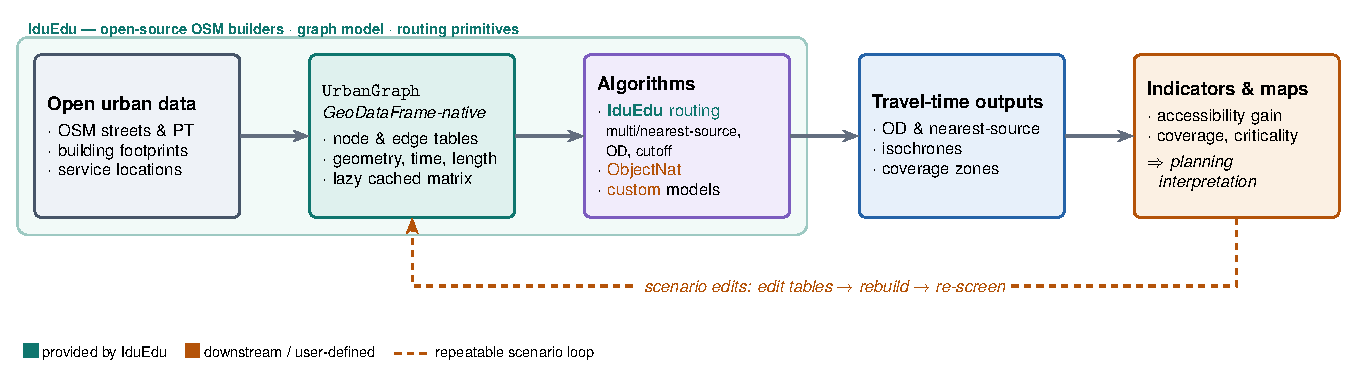
\includegraphics[width=\textwidth]{figures/workflow_figure}
        \caption{Analytical workflow instantiated in this paper. Open urban data are converted into a
        GeoDataFrame-native \texttt{UrbanGraph}, whose canonical node and edge tables also serve as the
        source of a lazily built computational form. Routing primitives provided by IduEdu, together
        with downstream (ObjectNat) or user-defined algorithms, turn the graph into travel-time outputs
            (OD and nearest-source tables, isochrone and coverage geometries) that are aggregated into
            accessibility indicators, maps and planning interpretation. Because scenarios are ordinary edits
            of the graph tables followed by a rebuild, the loop can be re-run for systematic screening.
            IduEdu provides the OSM builders, the graph model and the routing primitives (shaded); domain
            algorithms and behavioral models plug in downstream.}\label{fig:workflow}
    \end{figure}

    \subsection{Problem Setting and Notation}
    \label{subsec:notation}

    Urban street and transport networks are modeled as a graph $G = (V, E)$ with vertex set $V$ and edge
    set $E$~\cite{trudeau1994graphtheory,barthelemy2011spatial,barthelemy2022spatial,newman2010networks}.
    Throughout this paper, $G$ is a spatial, weighted, directed (multi)graph, represented for numerical
    computation by a sparse adjacency matrix.
    In the street network, vertices correspond to intersections, junctions or dead ends and carry point
    geometry; edges correspond to street segments and carry both topology and a linestring geometry
    reflecting the actual road shape, together with length and travel-time attributes.
    Combining topology with geometry is essential for spatial analysis and transport
    modeling~\cite{barthelemy2011spatial,boeing2025osmnx}.

    For public transport, the graph is extended with specialized vertices (surface stops, platforms,
    subway entrances and exits) and edges (transit segments between consecutive stops, and transfer
    edges representing boarding, alighting and interchanges).
    A central computational task is the calculation of OD matrices containing shortest-path values
    between sets of origin and destination vertices; in applied studies, origins typically correspond to
    residential locations and destinations to opportunities such as jobs, schools or transit
    stops~\cite{foti2014pandana,liu2022accessibility}.
    Computing a full OD matrix is expensive for large, detailed graphs~\cite{kwan1998accessibility}, but
    many accessibility questions only concern reachability within a bounded travel-time budget; a cutoff
    threshold then yields a sparse OD matrix at a fraction of the cost without losing the information
    relevant to the analysis.

    \subsection{UrbanGraph: A GeoDataFrame-Native Dual Representation}
    \label{subsec:urban_graph}

    The central design principle of IduEdu is that the storage and computational representations of the
    network coincide.
    An \texttt{UrbanGraph} consists of two \texttt{GeoDataFrame} tables: a node table with point
    geometry, and an edge table with mandatory attributes \texttt{u}, \texttt{v}, \texttt{geometry},
    \texttt{length\_meter} and \texttt{time\_min}; parallel edges of the multigraph are distinguished by
    an integer key \texttt{k}, and directionality is encoded by a boolean \texttt{oneway} column.
    Numerical computations run on a compressed sparse row (CSR) adjacency
    matrix~\cite{virtanen2020scipy} that is built directly from the edge table by vectorized operations,
    cached on the graph object, and invalidated (or explicitly rebuilt via
    \texttt{update\_adjacency\_matrix}) when the tables change structurally.
    The tabular geometric form is canonical; the CSR matrix is a derived, cached computational view.

    This design has two practical consequences.
    First, node and edge attributes are stored column-wise, which keeps the representation compact
    (Section~\ref{subsec:res-build}) and allows vectorized pandas/GeoPandas operations over the whole
    graph without iterating Python objects.
    Second, the graph is directly compatible with the geospatial analysis ecosystem: the analyst can
    filter and group edges, perform spatial joins, reproject, visualize with
    \texttt{.plot()}/\texttt{.explore()}, add custom attributes and edge costs, modify or delete edges,
    and validate the graph afterwards---all with ordinary GeoPandas code, without traversing nested
    dictionaries.
    By contrast, in NetworkX-based stacks geometry and transport attributes live as Python object
    attributes and must be extracted into tables for bulk geospatial operations, and the graph must
    additionally be converted into a specialized backend before fast computation; convenience and
    performance thus require two separate sources of truth.

    Listing~\ref{lst:tablefirst} illustrates the resulting workflow: a scenario is defined by an
    ordinary boolean mask over the edge table, the cached CSR is rebuilt, and the same routing primitive
    is re-executed.
    This mechanism underlies the scenario experiments of Section~\ref{subsec:scenarios}.
    The same tables also serve as an extensibility point: custom route-choice logic, mode preferences or
    behavioral mobility models developed in other studies can be implemented over the tabular attributes
    and computational primitives without changing the canonical representation of the network.

    \begin{listing}[H]
        \caption{Table-first scenario workflow: a service-degradation scenario expressed as a GeoPandas mask
        over \texttt{edges\_gdf}, followed by CSR rebuild and re-routing.\label{lst:tablefirst}}
        \rule{\columnwidth}{1pt}
        \raggedright\small
        \begin{verbatim}
from iduedu import get_intermodal_graph

g = get_intermodal_graph(polygon=aoi)           # UrbanGraph from OSM

edges = g.edges_gdf                             # ordinary GeoDataFrame
mask = (edges["type"] == "boarding") & (edges["route"] == "1")
edges.loc[mask, "time_min"] += 5.0              # +5 min modeled waiting

g.update_adjacency_matrix(weight="time_min")    # rebuild cached CSR

nearest = g.multi_source_dijkstra_nearest_source(
    gdf_sources=schools, weight="time_min", reverse=True)
        \end{verbatim}
        \rule{\columnwidth}{1pt}
    \end{listing}

    \subsection{Street Network Construction from OpenStreetMap}
    \label{subsec:street-construction}

    IduEdu extracts street networks from OSM via the Overpass API~\cite{overpass_api}.
    For each network type, a query is formed with the polygon of the study area and filters over
    \texttt{way} objects, yielding linear features with geometry and OSM attributes (travel direction,
    speed limits, etc.).
    Way-node coordinates are assembled into linestring collections using vectorized
    \texttt{numpy}~\cite{harris2020numpy} operations and \texttt{shapely.linestrings}~\cite{shapely},
    and the geometry is projected to the local UTM zone for correct length computation.

    An important construction step is network simplification.
    OSM linear features contain intermediate vertices that do not correspond to functional network
    points; keeping them inflates the graph.
    Edge simplification and node consolidation produce a more faithful representation of the street
    structure, reduce algorithmic complexity and accelerate downstream computation without losing
    accuracy~\cite{boeing2025osmnx}.
    In IduEdu, simplification is performed with \texttt{shapely.line\_merge}, which merges linestrings
    that touch only at their endpoints into longer segments; simplification thus operates at the level
    of spatial operations, avoiding explicit vertex-by-vertex iteration in Python.
    Figure~\ref{fig:simplify} shows an example before and after simplification.

    \begin{figure}[H]
        \centering
        
\includegraphics[width=10.5cm]{figures/simplify_comparison}
        \caption{Street network before (\textbf{left}) and after (\textbf{right}) edge simplification.
        Simplification removes intermediate vertices that do not correspond to functional network nodes
        while preserving topology and geometry.\label{fig:simplify}}
    \end{figure}

    After simplification, the graph structure is built.
    For the road network, travel direction is respected: edges not marked as one-way are duplicated in
    the reverse direction.
    Speeds are taken from \texttt{maxspeed} attributes where present, otherwise assigned by road class;
    edge travel time follows from segment length and assigned speed.
    The result is a directed, weighted \texttt{UrbanGraph} multigraph whose node and edge tables are
    formed vectorized from coordinate arrays, without intermediate object structures.
    The walk graph is built analogously, with all edges bidirectional.

    \subsection{Public Transport and Multimodal Graph Construction}
    \label{subsec:pt-construction}

    For a given territory and a set of supported transport modes, IduEdu extracts the corresponding OSM
    \texttt{relation} objects together with the associated street elements and stop infrastructure.
    For subways, stations, platforms and interchange groups (\texttt{stop\_area},
    \texttt{stop\_area\_group}) are additionally requested, allowing underground passages and
    entrances/exits to be represented.

    Each PT route, represented in OSM as a relation, is converted into a graph structure: the elements
    defining the vehicle's path along the street network are separated from stop and platform points
    where passengers board and wait.
    OSM PT data are not strictly validated---routes may be fragmentary, path geometry broken, and stops
    or platforms partially missing---so IduEdu reconstructs a continuous route path and a
    stop--platform pairing for every route segment.
    From the continuous geometry, a directed graph is formed in which vertices correspond to stops and
    platforms and edges to travel segments between consecutive stops (Figure~\ref{fig:pt_multimodal},
    left).
    Boarding edges connect stops to their platforms; their weight is configurable and defaults to
    1~min, modeling boarding and waiting.
    Travel-edge weights are computed from segment length and an effective speed that depends on
    configurable per-mode characteristics and street-network constraints.

    For subways, the graph is extended with links between station entrances/exits, platforms and
    boarding points.
    Where OSM records station depth, entrance/exit edge times account for vertical movement (escalators
    or elevators), providing a practical heuristic for the effect of station depth on total access
    time.
    After processing all routes, the per-route graphs are merged into a single PT graph; platforms
    shared by several routes or modes are merged into common vertices, enabling correct transfer
    modeling.
    Finally, the PT graph is integrated with the walk network: each platform or subway access
    point is matched to the nearest walk edge within a given radius and projected onto its geometry,
    splitting the edge in two without changing total walk weights (Figure~\ref{fig:pt_multimodal},
    right).

    Two modeling conventions deserve emphasis.
    First, the PT graph is \emph{static}: it encodes route topology and modeled travel times, not
    timetables.
    Second, boarding-edge costs represent \emph{modeled waiting time}---a scenario parameter that can be
    tied to half the headway where service intervals are known~\cite{gogousou2026mobilityoracle}, not a
    quantity recovered from schedules.
    All results in this paper should therefore be read as \emph{structural accessibility under modeled
    travel times}, as distinct from timetable-aware, experienced accessibility.
    Table~\ref{tab:assumptions} consolidates the model assumptions.

    \begin{figure}[H]
        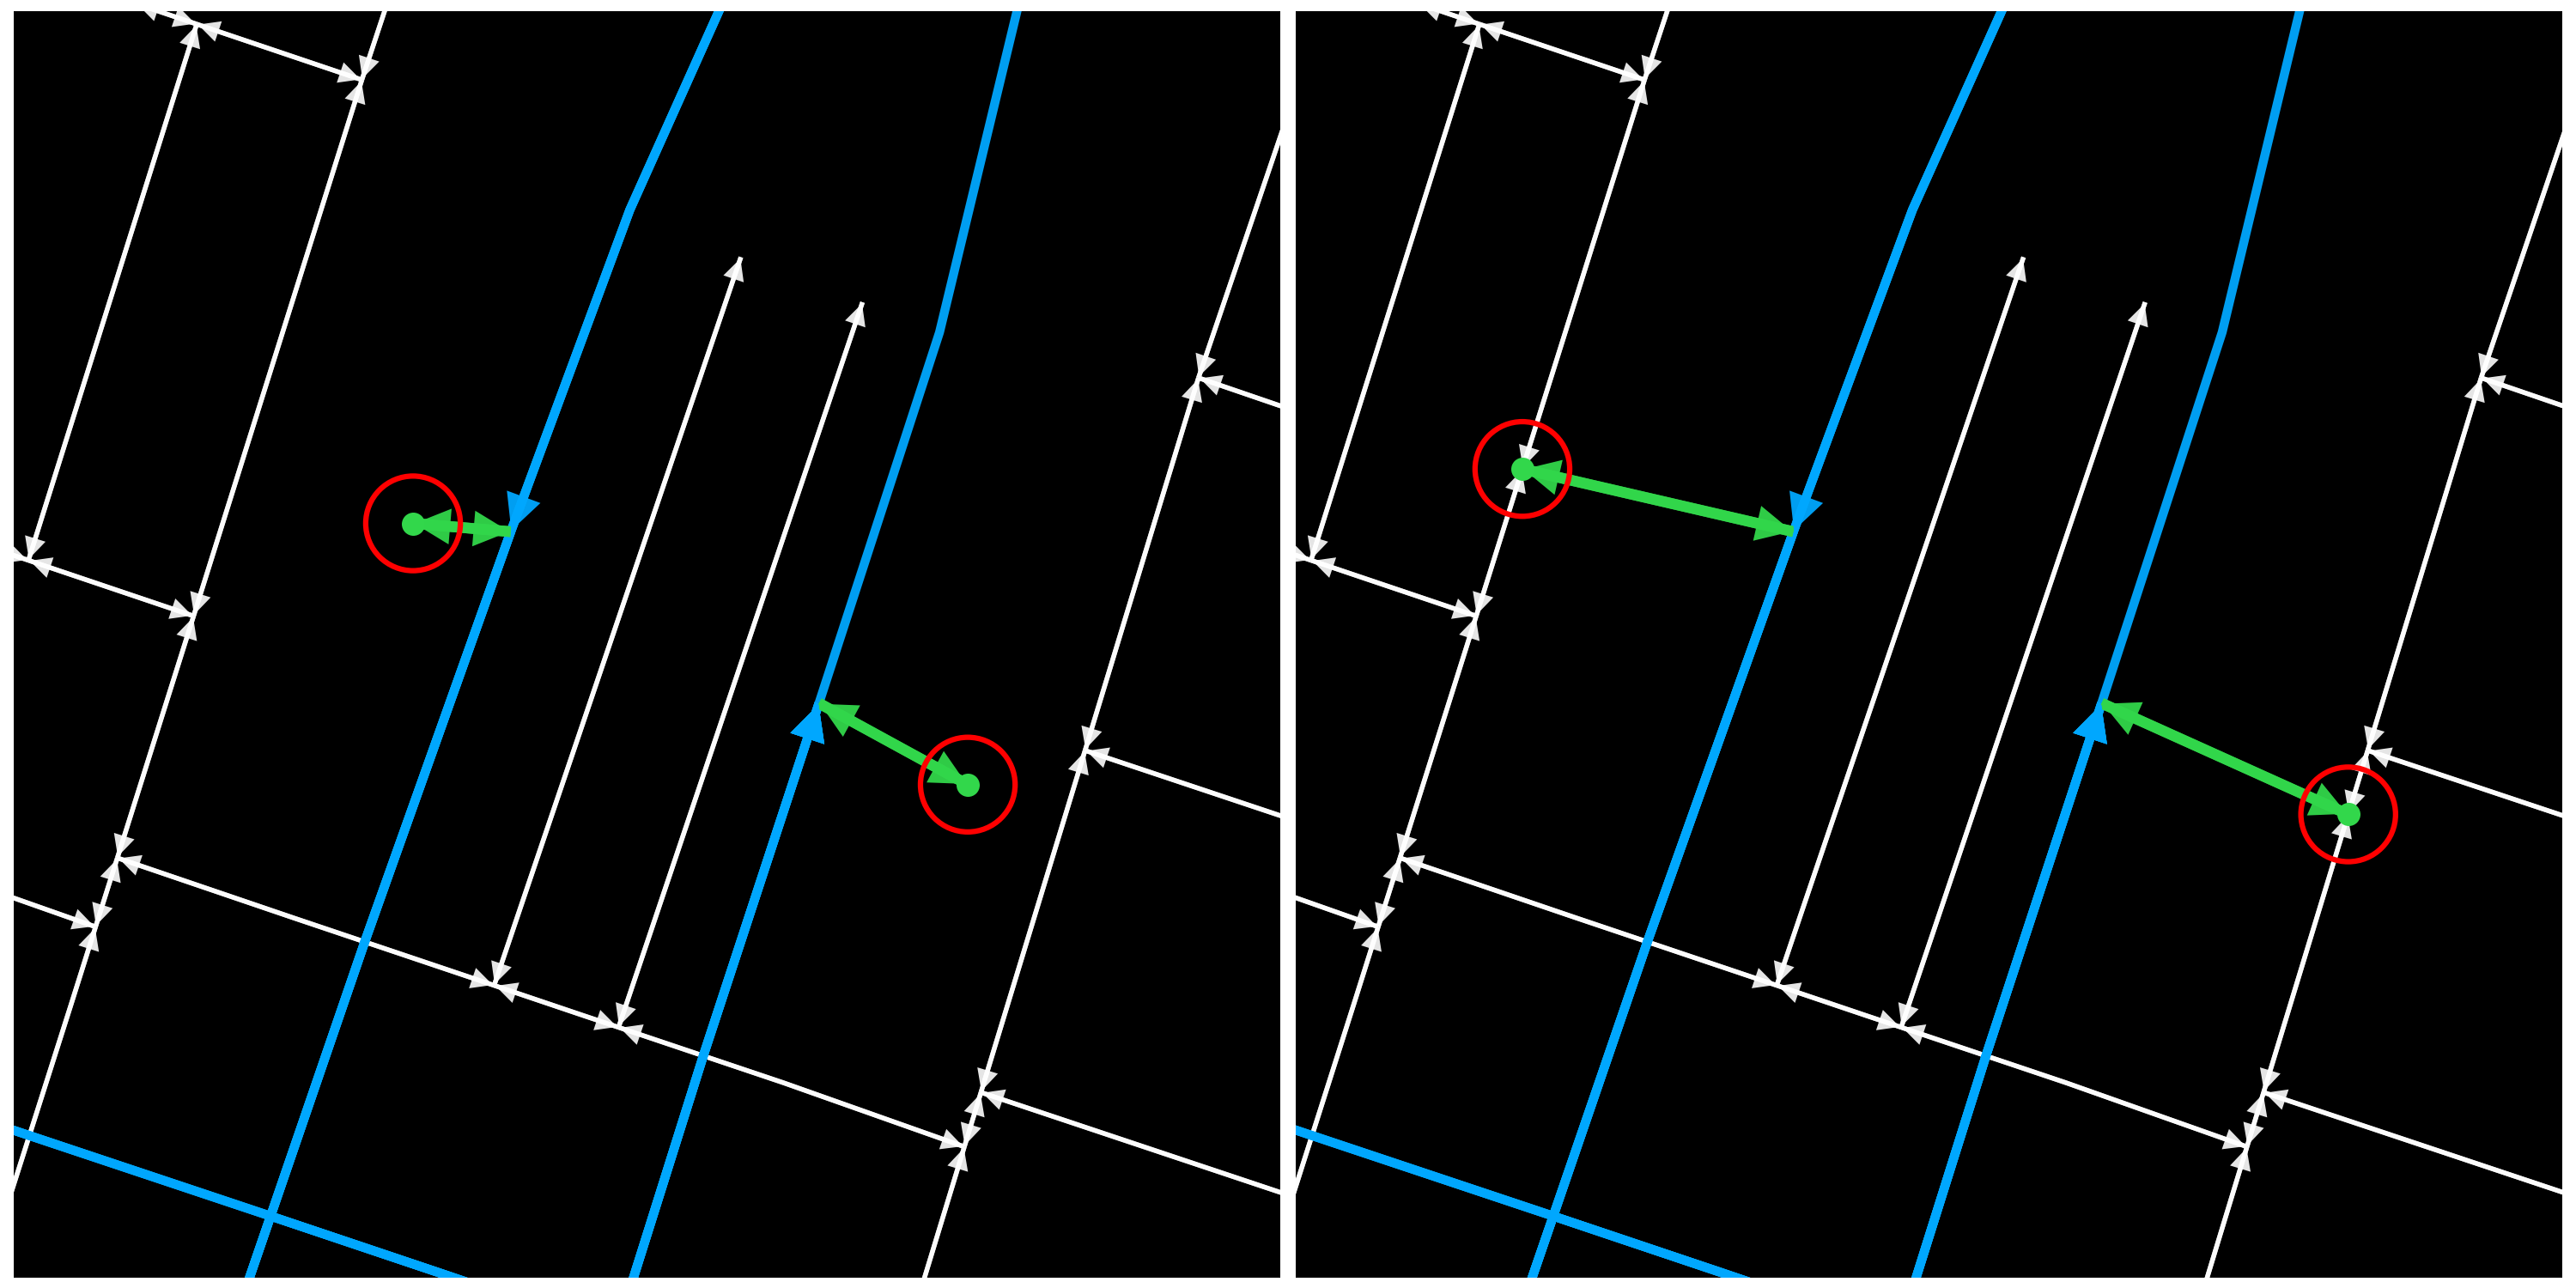
\includegraphics[width=\textwidth]{figures/pt_multimodal_example}
        \caption{Multimodal graph construction.
            (\textbf{Left}) The walk graph and the bus-route graph as separate networks.
            (\textbf{Right}) The resulting multimodal graph, in which PT platforms and stops are projected onto
            walk edges.\label{fig:pt_multimodal}}
    \end{figure}

    \begin{table}[H]
        \caption{Model assumptions and parameters of the case study.\label{tab:assumptions}}
        \begin{tabularx}{\textwidth}{lCC}
            \toprule
            \textbf{Parameter}    & \textbf{Value}                                                                                                      & \textbf{Observed/Modeled}    \\
            \midrule
            Walking speed         & 5 km/h                                                                                                              & modeled                      \\
            \midrule
            PT travel time        & kinematic per-mode model: $v_{\max}\times$ traffic coefficient, acceleration/braking losses, street speed-limit cap & modeled\\
            \midrule
            Boarding/waiting cost & 1 min baseline; $+5$/$+10$ min in degradation scenarios                                                            & modeled (scenario parameter) \\
            \midrule
            Subway station access & entrance/exit edges; vertical time from OSM station depth where recorded & observed + modeled\\
            \midrule
            Accessibility cutoffs & 15/30/45/60 min                                                                                                     & analysis choice              \\
            \midrule
            OSM data              & Overpass API, July 2026 snapshot                                                                                    & observed                     \\
            \bottomrule
        \end{tabularx}
    \end{table}

    \subsection{Routing Primitives}
    \label{subsec:routing}

    OD matrices are one output of the computational layer, not its only mode of operation.
    \texttt{UrbanGraph} exposes a family of routing primitives, all operating on the cached CSR
    representation with \texttt{float32} weights and JIT-compiled Numba kernels~\cite{lam2015numba}:

    \begin{itemize}
        \item \texttt{single\_source\_dijkstra\_path\_length} --- travel times from one vertex to all
        reachable vertices, optionally bounded by a cutoff;
        \item \texttt{multi\_source\_dijkstra\_path\_length} --- the combined shortest-path field of a
        set of sources, used for coverage-style questions;
        \item \texttt{multi\_source\_dijkstra\_nearest\_source} --- for every reachable vertex, the
        nearest source and the travel time to it; with \texttt{reverse=True} the search runs against
        edge direction, i.e., \emph{from} destinations (e.g., schools) backwards, yielding catchment
        assignments in one pass;
        \item \texttt{dijkstra\_path\_length\_parallel} --- independent per-source searches executed in
        parallel, used for per-origin isochrones;
        \item \texttt{od\_matrix} --- batch OD computation between two sets of spatial objects.
    \end{itemize}

    Spatial objects given as GeoDataFrames are snapped to their nearest graph vertices through the
    persistent R-tree index of the node table.
    For OD computation, the cardinalities of the origin and destination sets are compared first: since
    one Dijkstra run from a vertex computes shortest paths to all vertices within its search front, an
    OD matrix between $n$ origins and $m$ destinations requires $\min(n,m)$ runs.
    When origins substantially outnumber destinations, the graph is reversed by transposing its sparse
    representation and the roles of the two sets are swapped---an adaptive optimization that leaves the
    resulting matrix unchanged.
    The bounded multi-source Dijkstra variant~\cite{dijkstra2022note} additionally supports a cutoff on
    path weight: search-front expansion stops beyond the threshold, which sharply reduces cost relative
    to a full all-pairs computation and matches the local-reachability semantics of most accessibility
    questions.

    \subsection{Accessibility Indicators}
    \label{subsec:indicators}

    The indicators below are defined for an arbitrary class of urban service objects; in the case study
    of this paper that class is schools, and the same definitions apply unchanged to clinics,
    kindergartens or any other set of destinations.
    Let $\mathcal{O}$ be the set of residential origins and $\mathcal{S}$ the set of service objects.
    For each origin $i \in \mathcal{O}$ and network mode
    $M \in \{\mathrm{walk}, \mathrm{multimodal}\}$, let $t_i^{M}$ denote the travel time to the nearest
    service object and
    \begin{equation}
        n_i^{M}(\tau) = \bigl|\{ s \in \mathcal{S} : t_{is}^{M} \le \tau \}\bigr|
    \end{equation}
    the number of service objects reachable within cutoff $\tau \in \{15, 30, 45, 60\}$~min.
    The effect of public transport is measured by the absolute and relative gains
    \begin{equation}
        \Delta t_i = t_i^{\mathrm{walk}} - t_i^{\mathrm{multimodal}},
        \qquad
        r_i = \frac{\Delta t_i}{t_i^{\mathrm{walk}}} \quad \text{(for finite } t_i^{\mathrm{walk}}\text{)},
    \end{equation}
    and by the opportunity gain
    $g_i(\tau) = n_i^{\mathrm{multimodal}}(\tau) - n_i^{\mathrm{walk}}(\tau)$.
    Each origin is classified at a reference cutoff into four classes: \emph{no effect} ($g_i = 0$),
    \emph{moderate} ($g_i > 0$ below both thresholds), \emph{substantial}
    ($g_i \ge \gamma_{\mathrm{abs}}$ or $g_i / n_i^{\mathrm{walk}} \ge \gamma_{\mathrm{rel}}$), and
    \emph{newly reachable} ($n_i^{\mathrm{walk}} = 0$, $n_i^{\mathrm{multimodal}} > 0$).
    Origins with no reachable service object in either network at the reference cutoff form a separate
    \emph{unreachable} class.
    The reference cutoff is 15~min---the walking scale at which the presence or absence of a PT effect
    is spatially most discriminative---while the narrative of Section~\ref{subsec:res-case} focuses on
    the 30- and 45-min budgets, where the opportunity effect is strongest.
    Class boundaries are fixed before analyzing results ($\gamma_{\mathrm{abs}} = 5$ objects,
    $\gamma_{\mathrm{rel}} = 25\%$); their sensitivity to alternative values is examined in
    Appendix~\ref{app:class-sensitivity}.
    Aggregate coverage indicators include the share of origins with at least one reachable service
    object within $\tau$ and isochrone/coverage areas in km\textsuperscript{2}.
    Because origins are not population-weighted, we interpret all results as \emph{structural
    accessibility of residential locations}, not as social equity measures.

    \subsection{Isochrone and Coverage Geometry via ObjectNat}
    \label{subsec:objectnat}

    Polygon-based views of the same routing results are produced with ObjectNat~2.0.
    We use \texttt{get\_graph\_isochrones} and \texttt{get\_stepped\_graph\_isochrones} for per-origin
    (stepped) isochrones, and \texttt{get\_graph\_coverage} and \texttt{get\_stepped\_graph\_coverage}
    for reverse-search catchments and stepped coverage zones of the destination set (the schools, in
    our case study).
    The single-origin comparison in Figure~\ref{fig:isochrones} uses the network-following
    \texttt{ways} construction. Stepped isochrones and coverage maps use \texttt{radius}, whose compact
    and stable polygons remain legible at the full-city scale.
    Isochrone and coverage geometries also yield areal indicators (zone areas, buildings inside zones
    per time step).

    \subsection{Scenario Definitions: Route Criticality and Service Degradation}
    \label{subsec:scenarios}

    A scenario is a formal transformation of the baseline edge table followed by CSR rebuild and
    re-computation of the same indicators; every scenario records a manifest (scenario ID, edge filter, changed parameters, baseline fingerprint).
    The two experiments below are complementary and are reported in the order in which they inform
    each other: the screening first establishes which routes carry the structural load, and the
    degradation experiment then probes service quality on one of them.

    \textbf{Leave-one-route-out screening.}
    For each major route $r$, a derived scenario removes its travel and boarding edges while keeping
    shared platforms and all other routes intact; isolated elements do not affect the computation.
    Routes are ranked by the loss of $\tau$-minute opportunities
    \begin{equation}
        L_r(\tau) = \sum_{i \in \mathcal{O}} \bigl( n_i^{\mathrm{base}}(\tau) - n_i^{(r)}(\tau) \bigr),
    \end{equation}
    by the number of affected origins
    $A_r(\tau) = |\{ i : n_i^{(r)}(\tau) < n_i^{\mathrm{base}}(\tau) \}|$, and by newly unreachable
    origins.
    This experiment measures the structural criticality of individual routes.

    \textbf{Parametric service degradation.}
    For a selected mode or a single route $r$, the boarding edges are located by an attribute mask
    (\texttt{type == "boarding"}) and their \texttt{time\_min} is
    increased by $\delta \in \{5, 10\}$~min.
    Where official headways are available, $\delta$ can be derived as half the headway
    increase~\cite{gogousou2026mobilityoracle}; otherwise the penalties are explicitly hypothetical
    sensitivity parameters.
    This experiment probes the sensitivity of accessibility to service quality.

    Neither experiment models timetables or passenger demand; both quantify how modeled structural
    accessibility responds to formally defined network changes.
    In the released artifacts the two scenario families carry the identifiers \texttt{p1\_*} and
    \texttt{p0\_*}, respectively.

    \subsection{Case Study Area, Data and Experimental Setup}
    \label{subsec:setup}

    The applied case study asks what an explicit multimodal network adds to a city-scale assessment of
    school accessibility from residential buildings in Saint Petersburg, Russia, relative to the
    walk-only network that current extraction tools provide, and how far that difference depends on
    individual modes and routes (RQ4).
    Origins are the 83{,}510 residential buildings of the city, selected from 168{,}886 building
    footprints. A balanced building-level population allocation is used only for the secondary
    population-weighted comparison of walk and multimodal coverage.
    Destinations are 911 schools extracted from OSM.
    The analysis area covers the city with a 1.2~km buffer, and all network and school data were
    retrieved from OSM via the Overpass API in July 2026.
    The resulting multimodal graph contains 533{,}650 nodes and 776{,}051 edges (the derived walk
    graph: 503{,}436 and 688{,}704); its PT layer includes all 635 urban PT routes---538 bus, 48
    trolleybus, 43 tram and 6 subway lines.

    The benchmark suite comprises: \textbf{B1} street graph construction against OSMnx and Pyrosm on
    six cities of increasing scale (Helsinki, Saint Petersburg, Moscow, London, Seoul, New York), with
    simplification on and off; \textbf{B2} multimodal construction (walk + PT + integration) on the same
    territories; \textbf{B3} OD computation against NetworKit and igraph on the Saint Petersburg
    multimodal graph, in rectangular ($|D| = 911$ schools) and square (origins-to-origins) settings;
    \textbf{B4} in-memory representation size; \textbf{B5} the accessibility case study; and \textbf{B6}
    the two scenario experiments.

    The OD comparison protocol reflects each tool's real workflow.
    Competing libraries start not from IduEdu's internal representation but from a
    \texttt{networkx.MultiDiGraph}---the standard representation produced by the OSMnx/NetworkX
    ecosystem---built from the same \texttt{UrbanGraph} (identical topology and weights, expanded
    one-way edges, preserved coordinates), so all tools route over the same network.
    Each competitor then pays the costs it pays in practice: conversion of the NetworkX graph into its
    own format (collapsing parallel edges by minimum weight) and spatial snapping of objects to vertices
    via its own \texttt{scipy.cKDTree} index.
    Convert and snap stages are measured separately from pure OD time; both pure and end-to-end times
    are reported.
    NetworkX itself does not participate as a router (it has no batch OD API); it serves only as the
    common source representation.
    IduEdu consumes its own \texttt{UrbanGraph} and snaps internally through the persistent R-tree
    index, so no conversion stage exists by construction.
    We report two comparison levels throughout: the pure OD kernel on an identical graph, and the
    end-to-end pipeline including snap/convert; the headline claim concerns the integrated workflow, not
    the universal superiority of any single shortest-path kernel.

    All experiments ran on a workstation with an Intel Core i7-12700F CPU and 64~GB RAM (Windows,
    Python 3.11.9).
    Key library versions: IduEdu~2.0.0, ObjectNat~2.0.0, OSMnx~2.1.0, Pyrosm~0.11.0, NetworkX~3.6.1,
    NetworKit~11.2.1, igraph~1.0.0, Numba~0.65.1, GeoPandas~1.1.4, Shapely~2.1.2, and SciPy~1.17.1;
    full per-run version lists are recorded in the repository's \texttt{env\_*.json} files.
    Every measurement was repeated at least three times; medians are reported and spreads are provided
    in the accompanying notebooks.
    Warm-up (Overpass cache population, Numba JIT compilation, library imports) preceded all
    measurements and is excluded from results.

%%%%%%%%%%%%%%%%%%%%%%%%%%%%%%%%%%%%%%%%%%


    \section{Results}
    \label{sec:results}

    The results follow the order of the research questions.
    Section~\ref{subsec:res-validity} verifies that the constructed representation is correct (RQ1);
    Sections~\ref{subsec:res-build}--\ref{subsec:res-ablations} measure what it costs to build and to
    compute over, and attribute that cost to individual design decisions (RQ2);
    Section~\ref{subsec:res-workflow} establishes that the resulting cost admits repeated city-scale
    analysis (RQ3); and Sections~\ref{subsec:res-case}--\ref{subsec:res-p0} report what the multimodal
    layer changes in such an analysis relative to a walk-only network (RQ4).

    \subsection{Graph and Public Transport Network Validity}
    \label{subsec:res-validity}

    Performance comparisons are meaningful only if the results coincide, so correctness is verified
    first.
    The IduEdu OD matrix is compared against a NetworkX reference computation on an identical graph:
    reachability sets coincide exactly, and the maximum discrepancy of finite values does not exceed
    $3\cdot10^{-4}$~min, attributable to rounding accumulation of the \texttt{float32} kernel relative
    to the \texttt{float64} reference.
    Second, walk graphs built by IduEdu and OSMnx for the same territory are compared: despite
    differing simplification rules, total network length agrees within ${\approx}1\%$, confirming
    equivalence of the extracted networks.

    Beyond numerical validity, we characterize the PT layer descriptively and compare it against the
    official route register of the city's transport authority.
    The multimodal graph of Saint Petersburg reconstructs 635 PT routes from OSM for the study
    period---538 bus, 48 trolleybus and 43 tram routes and 6 subway lines---represented by 28{,}000
    travel edges (23{,}605 bus, 2{,}523 trolleybus, 1{,}738 tram, 134 subway), 29{,}342 boarding and
    29{,}342 alighting edges, and 663 subway-infrastructure edges (entrances, exits and in-station
    transfers).
    Table~\ref{tab:pt_validity} sets these counts against the figures published by the Saint
    Petersburg public-transport authority (\emph{Organizator Perevozok})~\cite{orgp_spb}.
    The electric modes and the metro match almost exactly---trolleybus and subway are identical (48
    and 6) and tram differs by three routes---while the bus layer overcounts by ${\approx}20\%$.
    The bus discrepancy is consistent with three well-understood effects: the 1.2~km analysis buffer
    reaches beyond the administrative boundary and captures suburban and Leningrad-Oblast services
    absent from the city register; OSM also contains commercial routes not listed by the authority;
    and route relations are tagged unevenly, so directional or terminal variants sharing one public
    number can appear as separate relations.
    The close agreement of the electric modes and metro---whose OSM tagging is cleaner and more
    stable---supports the structural realism of the reconstructed network; the bus overcount is a
    counting artifact of OSM heterogeneity rather than of the graph builder.

    \begin{table}[H]
        \caption{Public transport routes in the reconstructed graph versus the official register of the
        Saint Petersburg transport authority (\emph{Organizator Perevozok}~\cite{orgp_spb},
            2026).\label{tab:pt_validity}}
        \begin{tabularx}{\textwidth}{lCCC}
            \toprule
            \textbf{Mode}  & \textbf{Official routes} & \textbf{IduEdu routes} & \textbf{Difference} \\
            \midrule
            Bus            & 447                      & 538                    & $+91$               \\
            Trolleybus     & 48                       & 48                     & $0$                 \\
            Tram           & 46                       & 43                     & $-3$                \\
            Subway (lines) & 6                        & 6                      & $0$                 \\
            \midrule
            Total          & 547                      & 635                    & $+88$               \\
            \bottomrule
        \end{tabularx}
    \end{table}

    \subsection{Street and Multimodal Graph Construction Performance}
    \label{subsec:res-build}

    In benchmark B1, walk and drive graph construction is compared across OSMnx, Pyrosm and
    IduEdu.
    The walk network is the most demanding case, with the largest vertex and edge counts due to
    detailed street infrastructure; the drive network adds directionality processing.
    To ensure comparability, all tools use the same area of interest: for each city an OSM PBF extract
    is downloaded, its header bounding box is extracted, and the same box is used as the geometric query
    for OSMnx and IduEdu.
    For OSMnx and IduEdu, runs with simplification enabled and disabled are compared; Pyrosm has no
    comparable switch.

    IduEdu consistently outperforms OSMnx on walk graphs.
    With simplification enabled, the median speedup across six cities is ${\approx}5.7\times$ (from
    $3.3\times$ on New York to $6.0\times$ on Helsinki); without simplification it rises to
    ${\approx}8.8\times$ (from $5.8\times$ on New York to $9.3\times$ on Moscow).
    In absolute terms, the Saint Petersburg walk graph builds in ${\approx}20$~s versus
    ${\approx}115$~s for OSMnx and ${\approx}95$~s for Pyrosm.
    For the drive network with simplification, the speedup over OSMnx is $3.3$--$5.1\times$ (median
    ${\approx}4.2\times$).
    Figure~\ref{fig:build_walk} summarizes the results.

    \begin{figure}[H]
        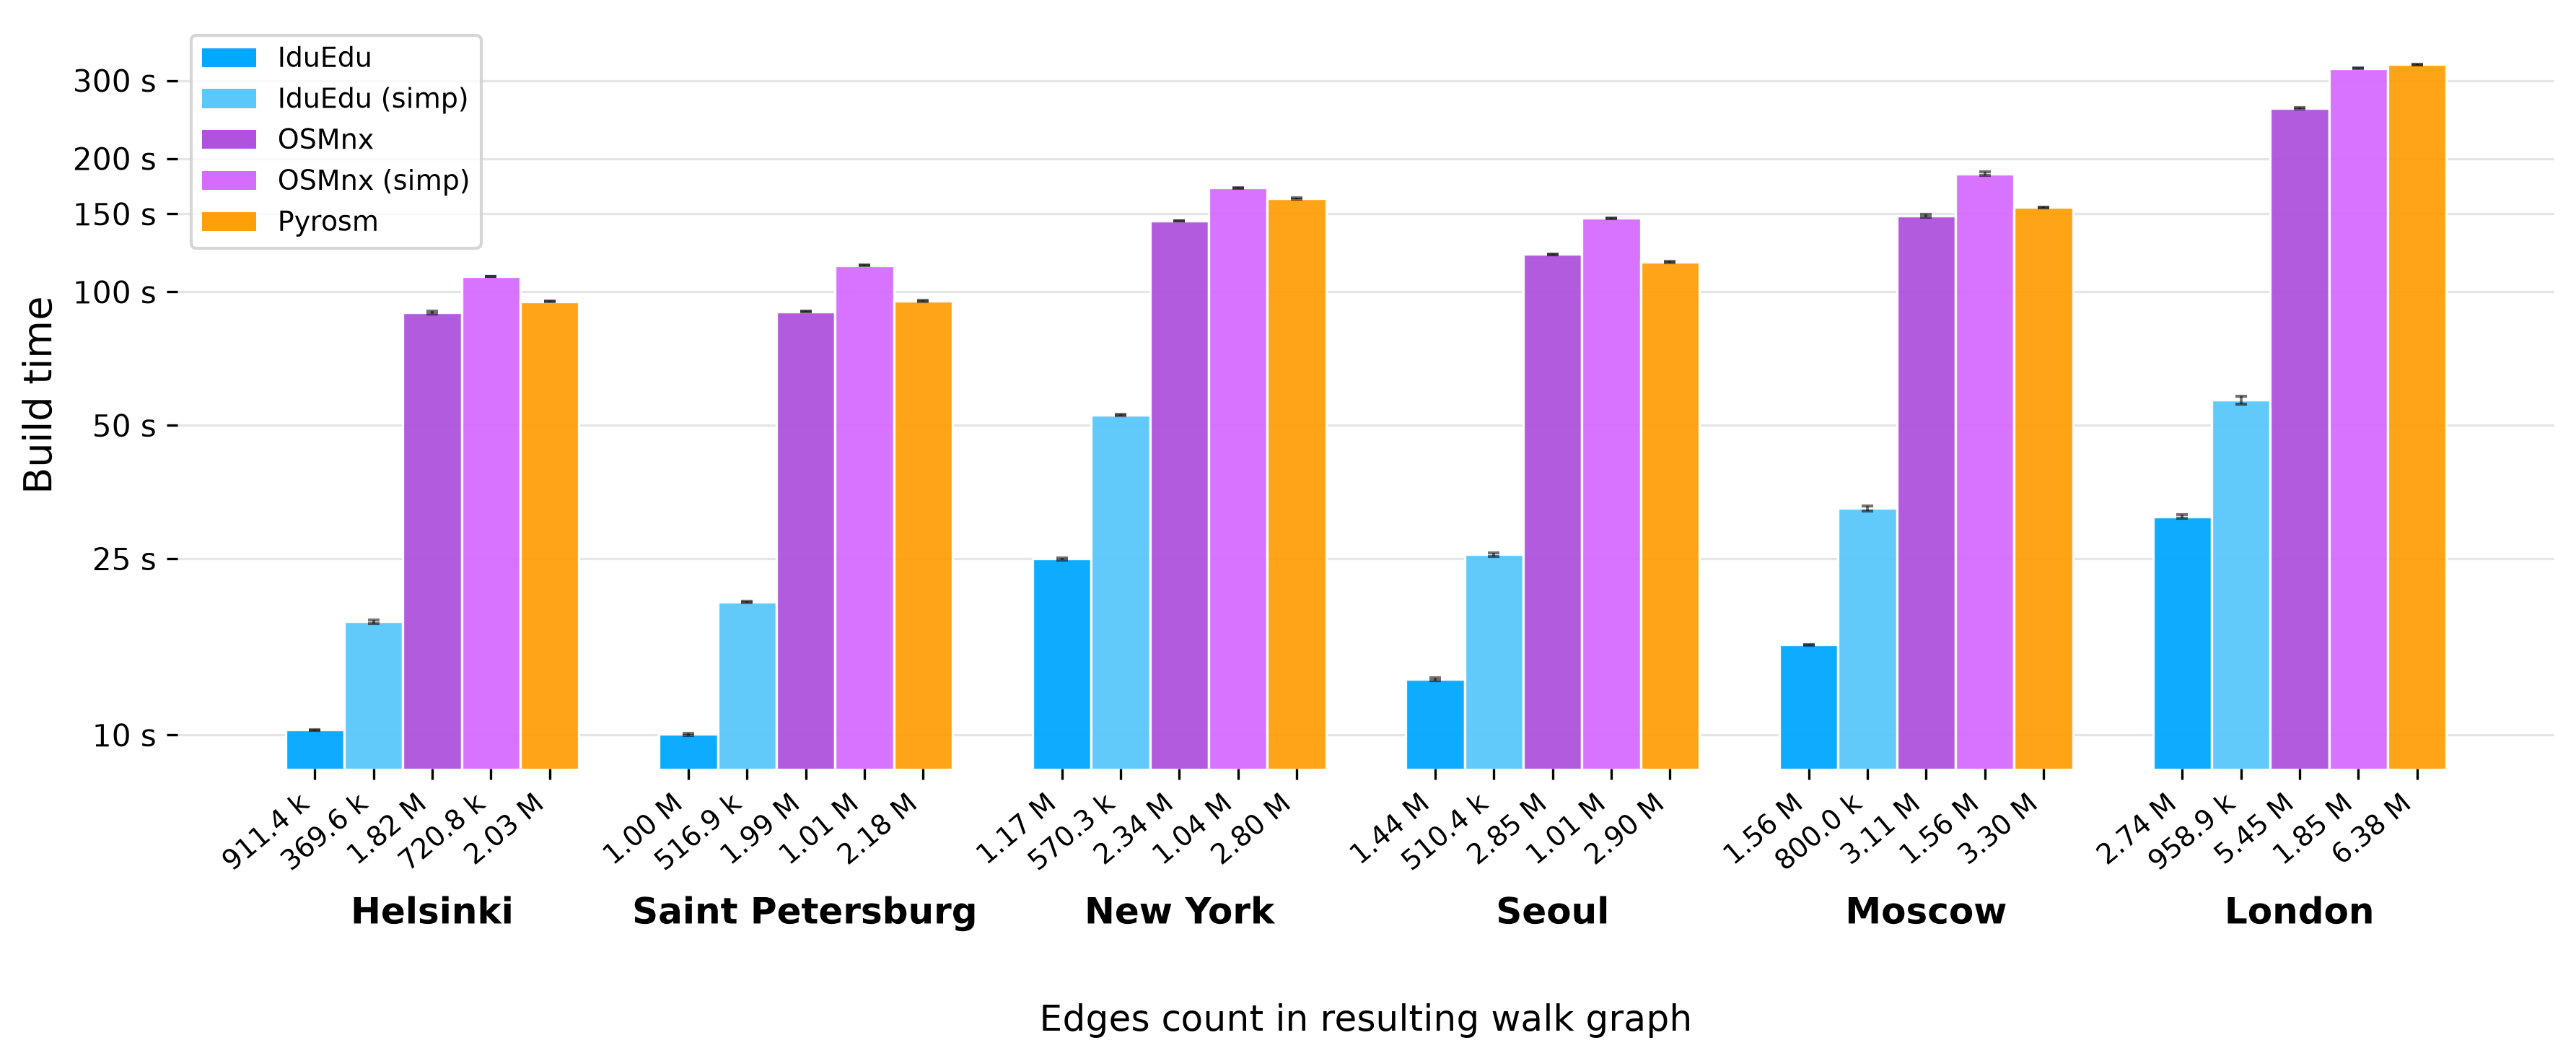
\includegraphics[width=\textwidth]{figures/build_benchmark_walk}
        \caption{Walk graph construction time and edge counts for OSMnx, Pyrosm and IduEdu across six
        cities, with simplification enabled and disabled.\label{fig:build_walk}}
    \end{figure}

    Benchmark B2 measures multimodal construction on the same territories: for each city, the
    walk graph, the PT graph (buses, trams, trolleybuses, subway) and their integration are built
    sequentially, with time and edge counts recorded per stage.
    Figure~\ref{fig:intermodal_build} decomposes total construction time into PT, walk and join stages
    across cities of different scale and network structure.

    \begin{figure}[H]
        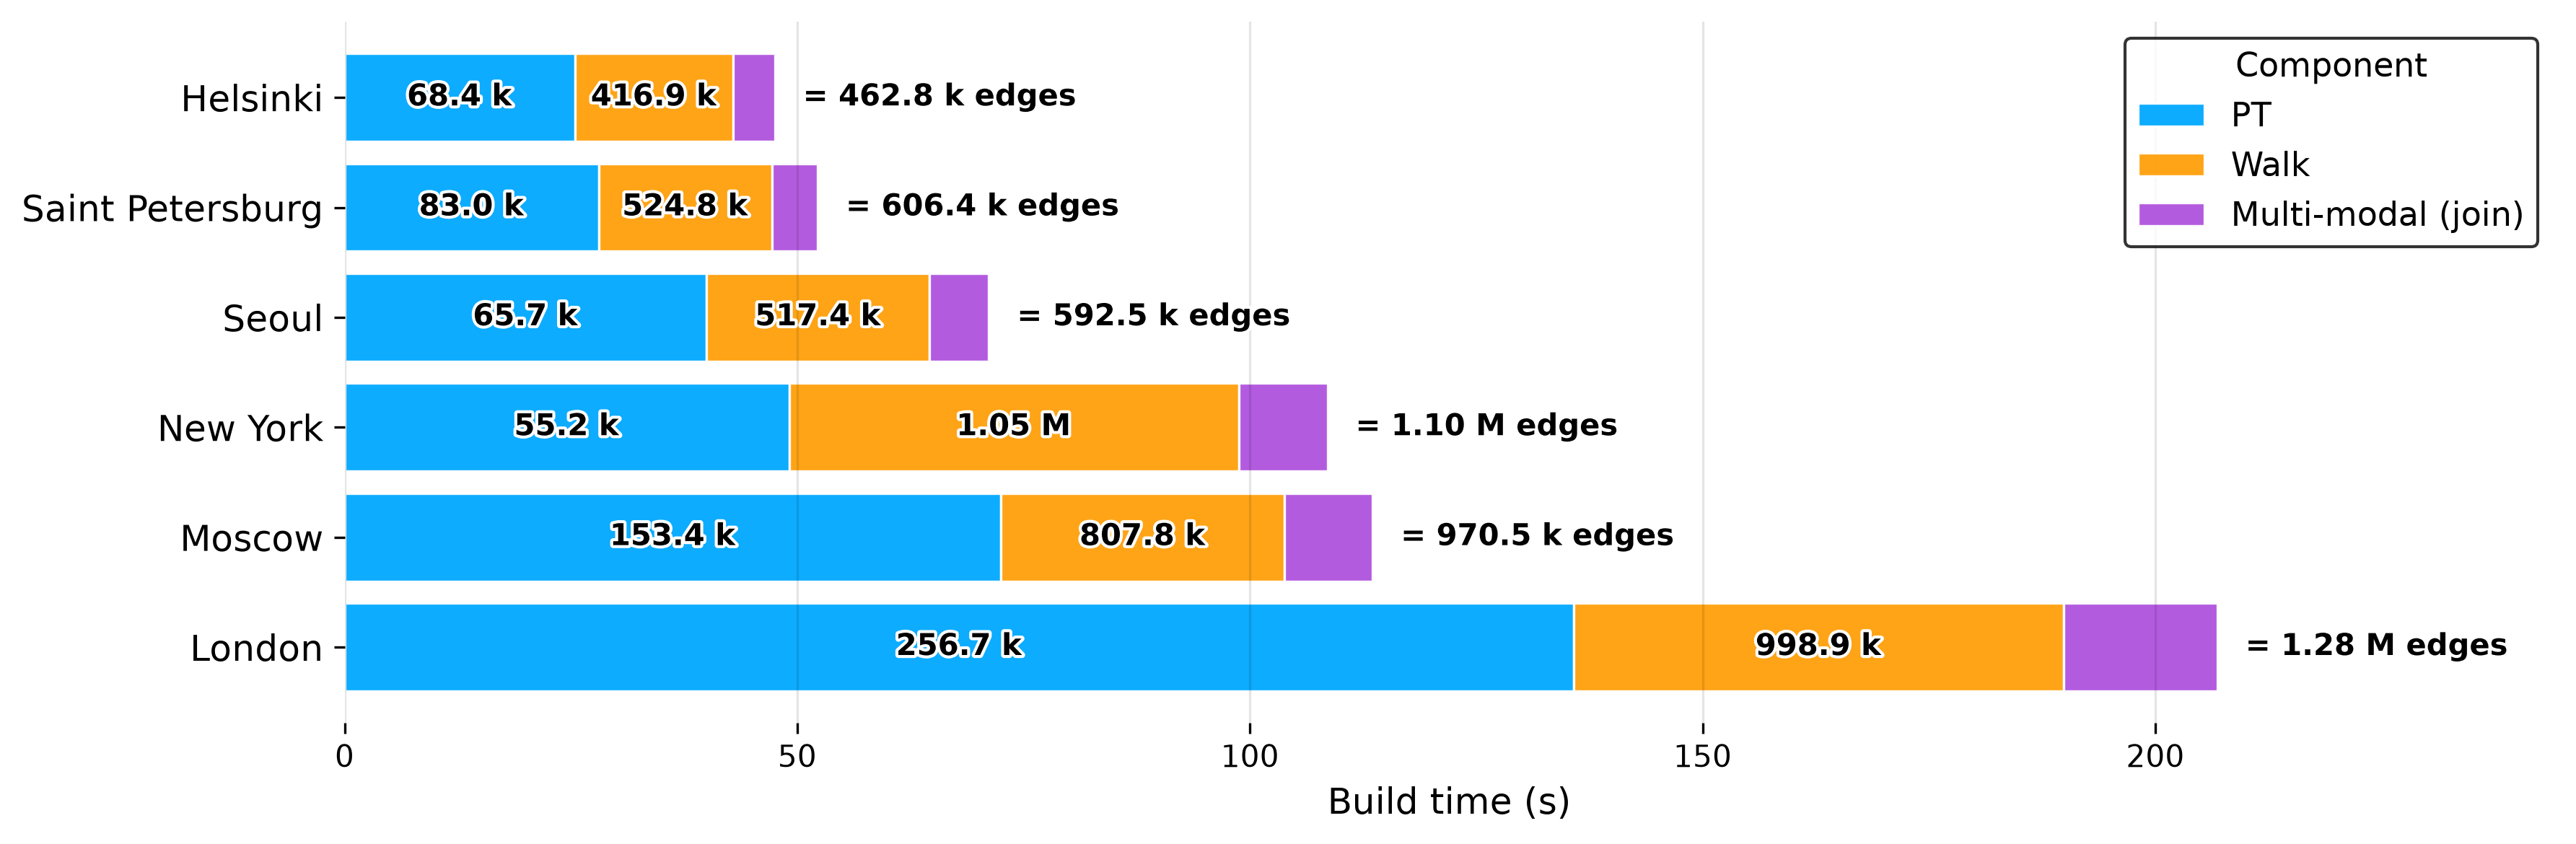
\includegraphics[width=\textwidth]{figures/intermodal_stacked_time_by_city}
        \caption{Multimodal graph construction time in IduEdu, decomposed into public transport (PT),
            walk and integration (Join) stages; labels give per-stage edge
            counts.\label{fig:intermodal_build}}
    \end{figure}

    The tabular representation affects not only speed but also memory.
    B1 additionally measures the deterministic in-memory size of the constructed graph representation:
    for IduEdu, the \texttt{UrbanGraph} object (node and edge GeoDataFrames including Shapely coordinate
    buffers); for OSMnx and Pyrosm, the returned \texttt{networkx.MultiDiGraph} with geometry and
    attributes.
    This protocol compares spatial graph representations, not geometry-free computational containers.
    As Figure~\ref{fig:memory} shows, columnar storage is substantially more compact at comparable
    spatial information content: for the Saint Petersburg walk graph (simplified),
    \texttt{UrbanGraph} occupies ${\approx}76$~MB versus ${\approx}865$~MB for the OSMnx
    \texttt{MultiDiGraph} (also simplified) and ${\approx}5.7$~GB for the raw, unsimplified Pyrosm
    graph.

    \begin{figure}[H]
        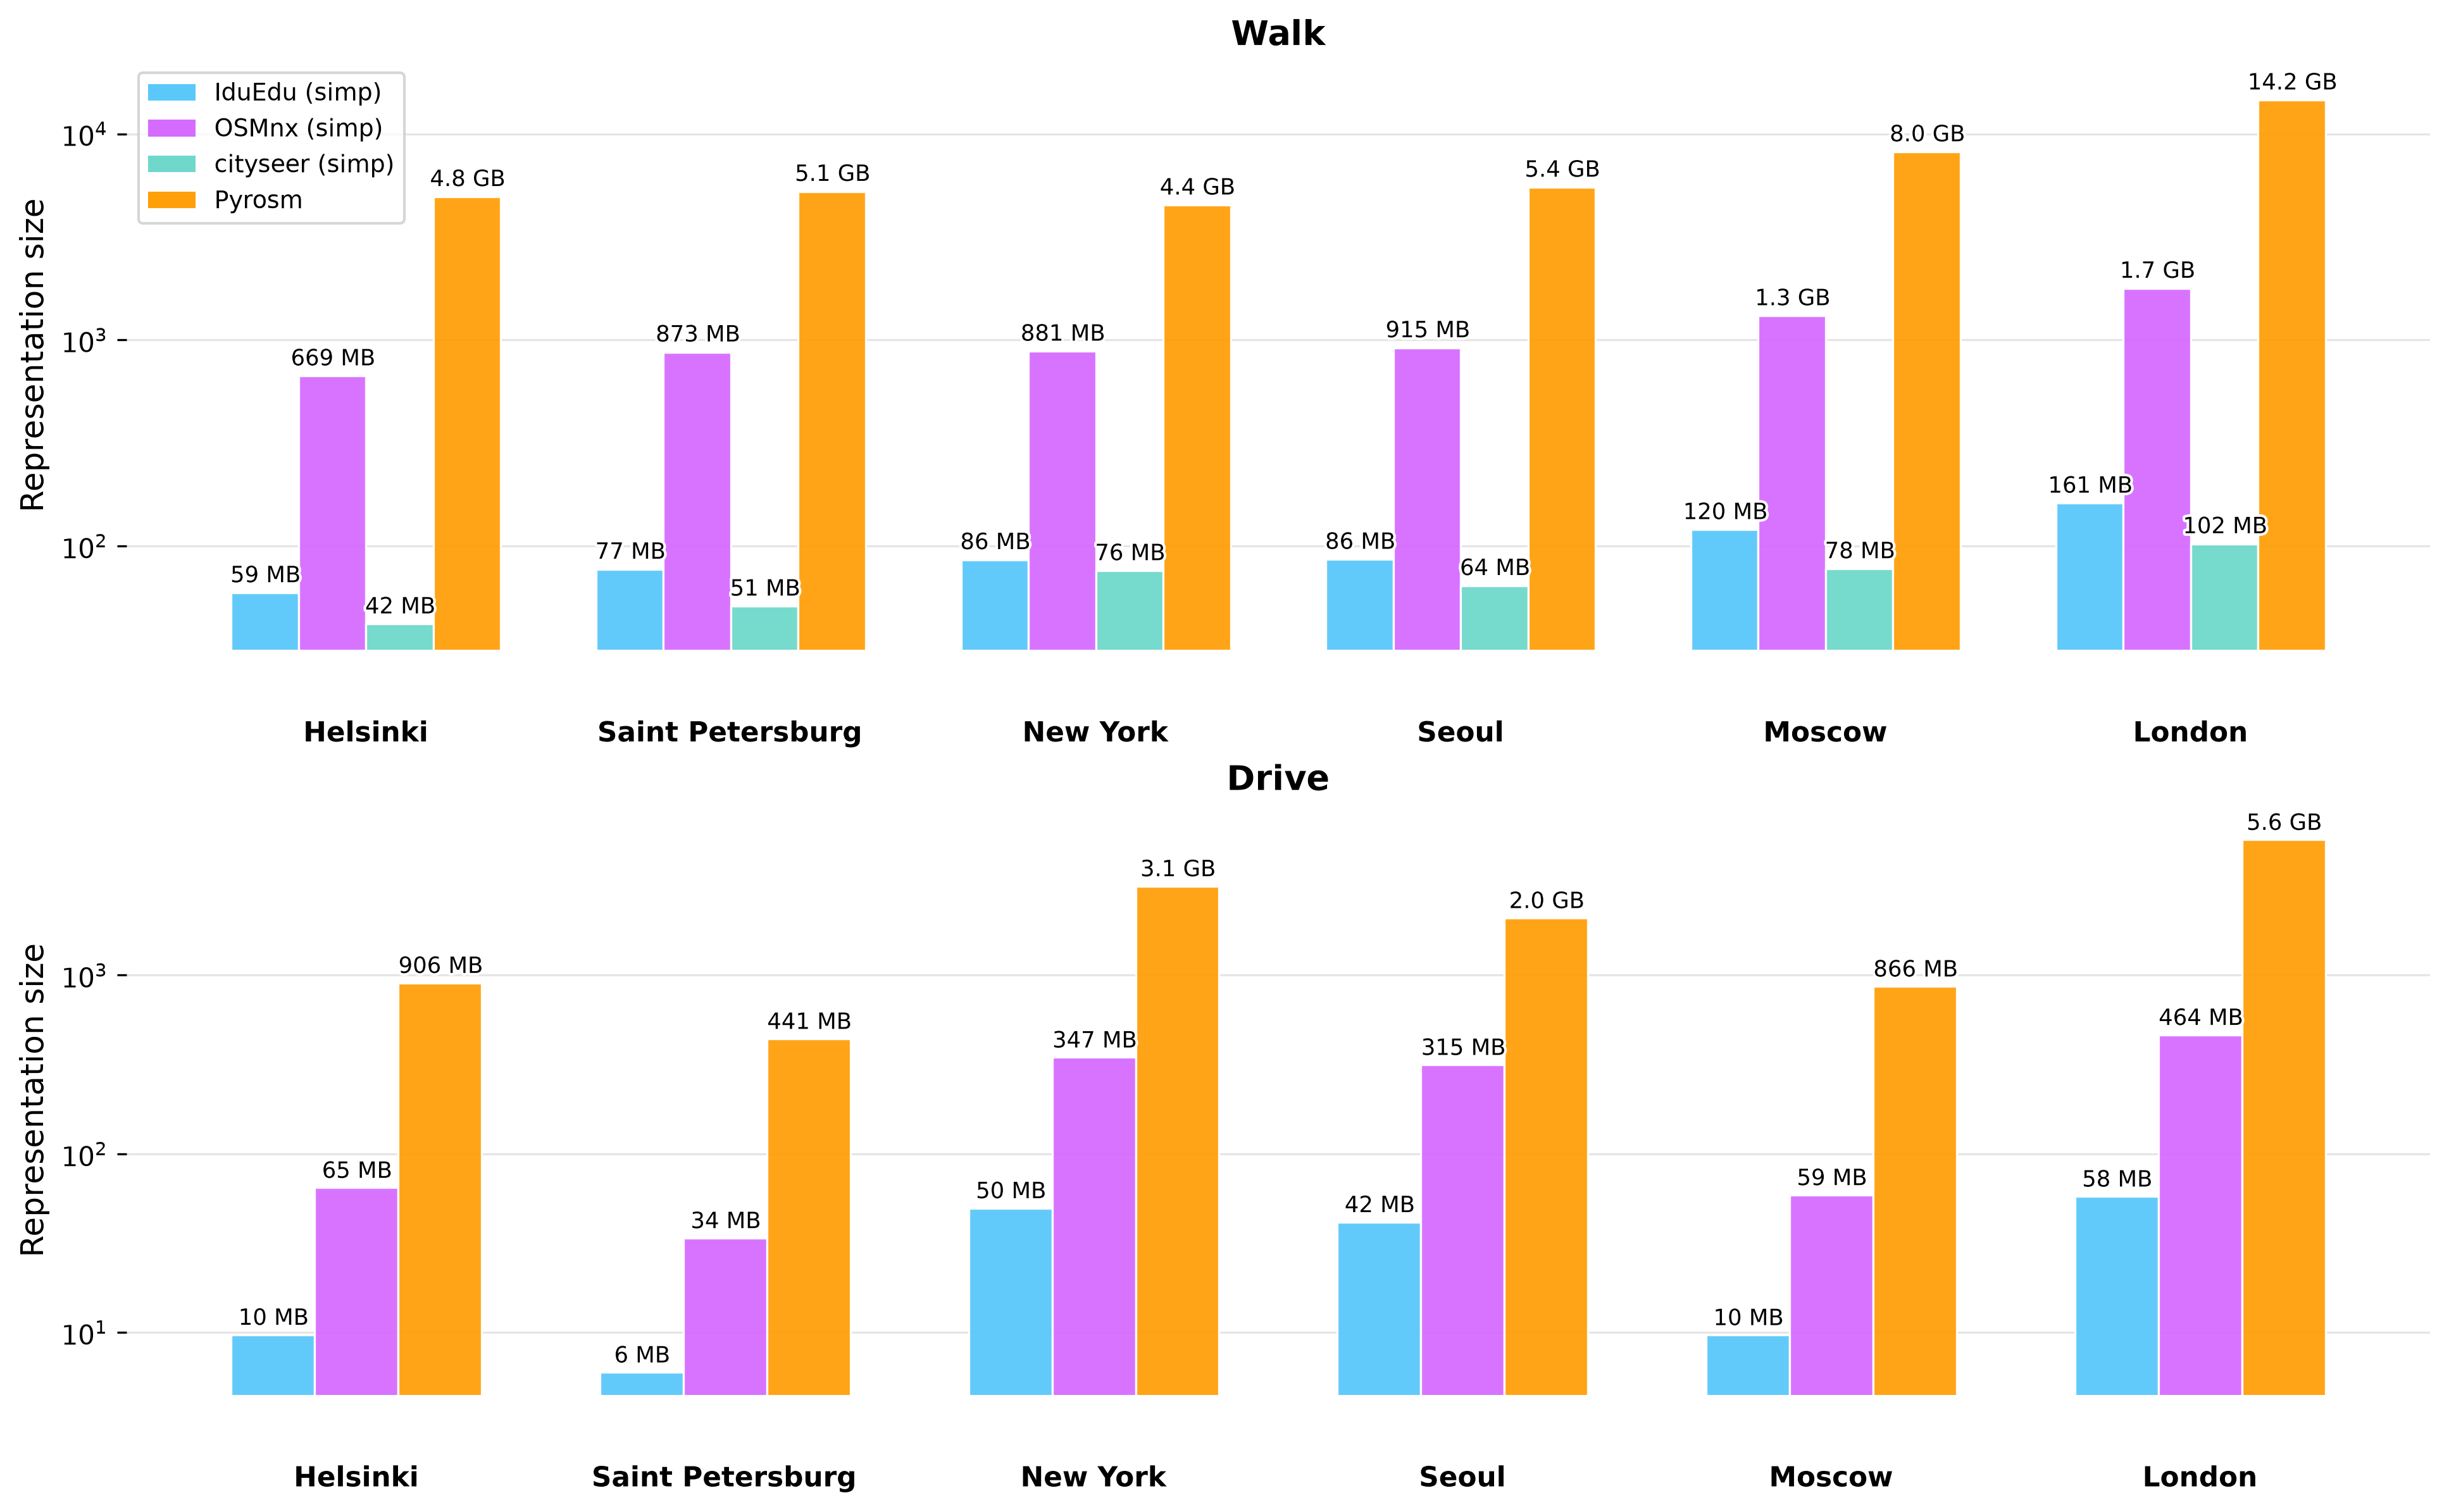
\includegraphics[width=\textwidth]{figures/memory_benchmark}
        \caption{In-memory graph representation size for IduEdu, OSMnx and Pyrosm (B1
        runs).\label{fig:memory}}
    \end{figure}

    \subsection{Routing Scalability: Batch OD Workloads}
    \label{subsec:res-od}

    Benchmark B3 compares OD computation time for IduEdu, NetworKit and igraph on the Saint Petersburg
    multimodal graph, weighted by travel time, under the fairness protocol of
    Section~\ref{subsec:setup}.
    The primary cross-library comparison is the \emph{full} mode: IduEdu without cutoff against
    NetworKit and igraph performing the same complete shortest-path computation.
    IduEdu cutoff curves are shown additionally; since NetworKit and igraph have no comparable
    bounded-search mechanism and always perform a full traversal, the cutoff mode should be read as a
    separate applied advantage on local-accessibility workloads rather than as part of the head-to-head
    comparison.

    Two settings separate the effect of origin/destination cardinality.
    In the \emph{rectangular} setting, origins are sampled from residential buildings and destinations
    are the fixed set of $|D| = 911$ schools; $|O|$ grows from 128 to 131{,}072, with identical subsets
    shared by all libraries and repetitions.
    As Figure~\ref{fig:od_rect} shows, the scaling behavior differs qualitatively: IduEdu's full-mode
    time grows weakly and stays within tens of seconds (${\approx}50$~s at $|O| = 1{,}024$ and
    ${\approx}80$~s at $|O| = 32{,}768$), whereas NetworKit and igraph exhibit nonlinear growth.
    The difference stems from adaptive graph reversal at $|O| > |D|$: the number of shortest-path runs
    is effectively determined by the smaller set.

    \begin{figure}[H]
        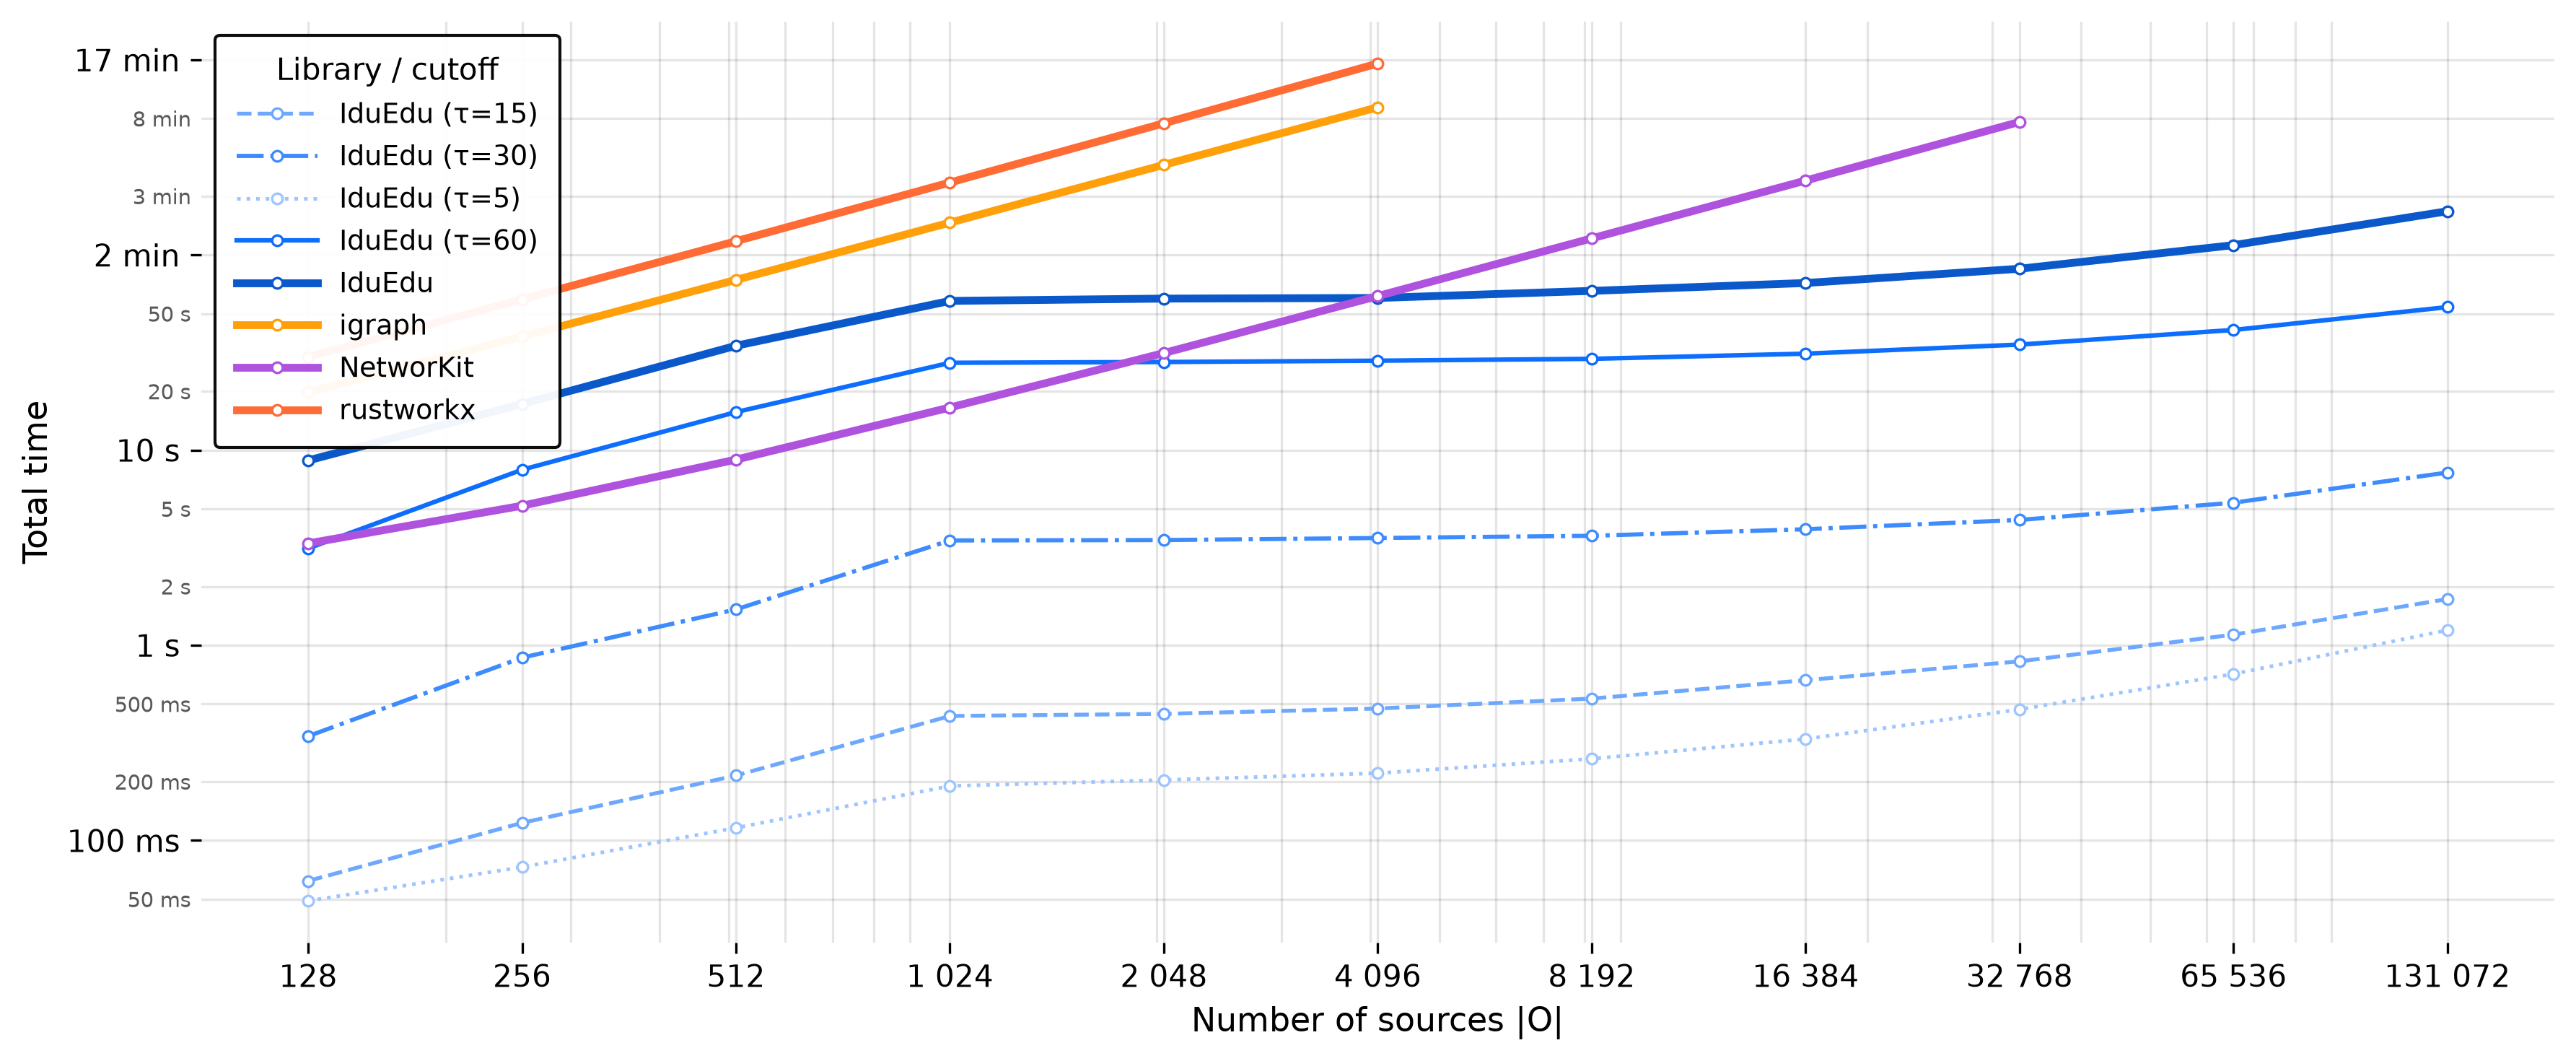
\includegraphics[width=\textwidth]{figures/od_time_rect}
        \caption{Rectangular OD computation time (origins $\to$ 911 schools) for IduEdu, NetworKit and
        igraph as a function of the number of origins; IduEdu curves for several cutoff values are shown
        separately.\label{fig:od_rect}}
    \end{figure}

    In the \emph{square} setting ($|O| = |D|$, origins-to-origins), a fixed random subsample of
    residential buildings serves as both origins and destinations.
    Graph reversal yields no benefit here, and complexity is governed directly by the number of
    sources.
    As Figure~\ref{fig:od_square} shows, in full mode IduEdu grows monotonically and falls behind
    NetworKit; introducing a cutoff qualitatively changes the behavior---at thresholds of 5--30 min,
    IduEdu's time depends only weakly on $|O|$, consistent with the growing share of out-of-radius
    pairs and the shrinking traversal depth.
    Due to practical runtime limits, igraph was run only for $|O| < 8{,}192$ and NetworKit for
    $|O| < 65{,}536$; IduEdu was measured at all sizes.

    \begin{figure}[H]
        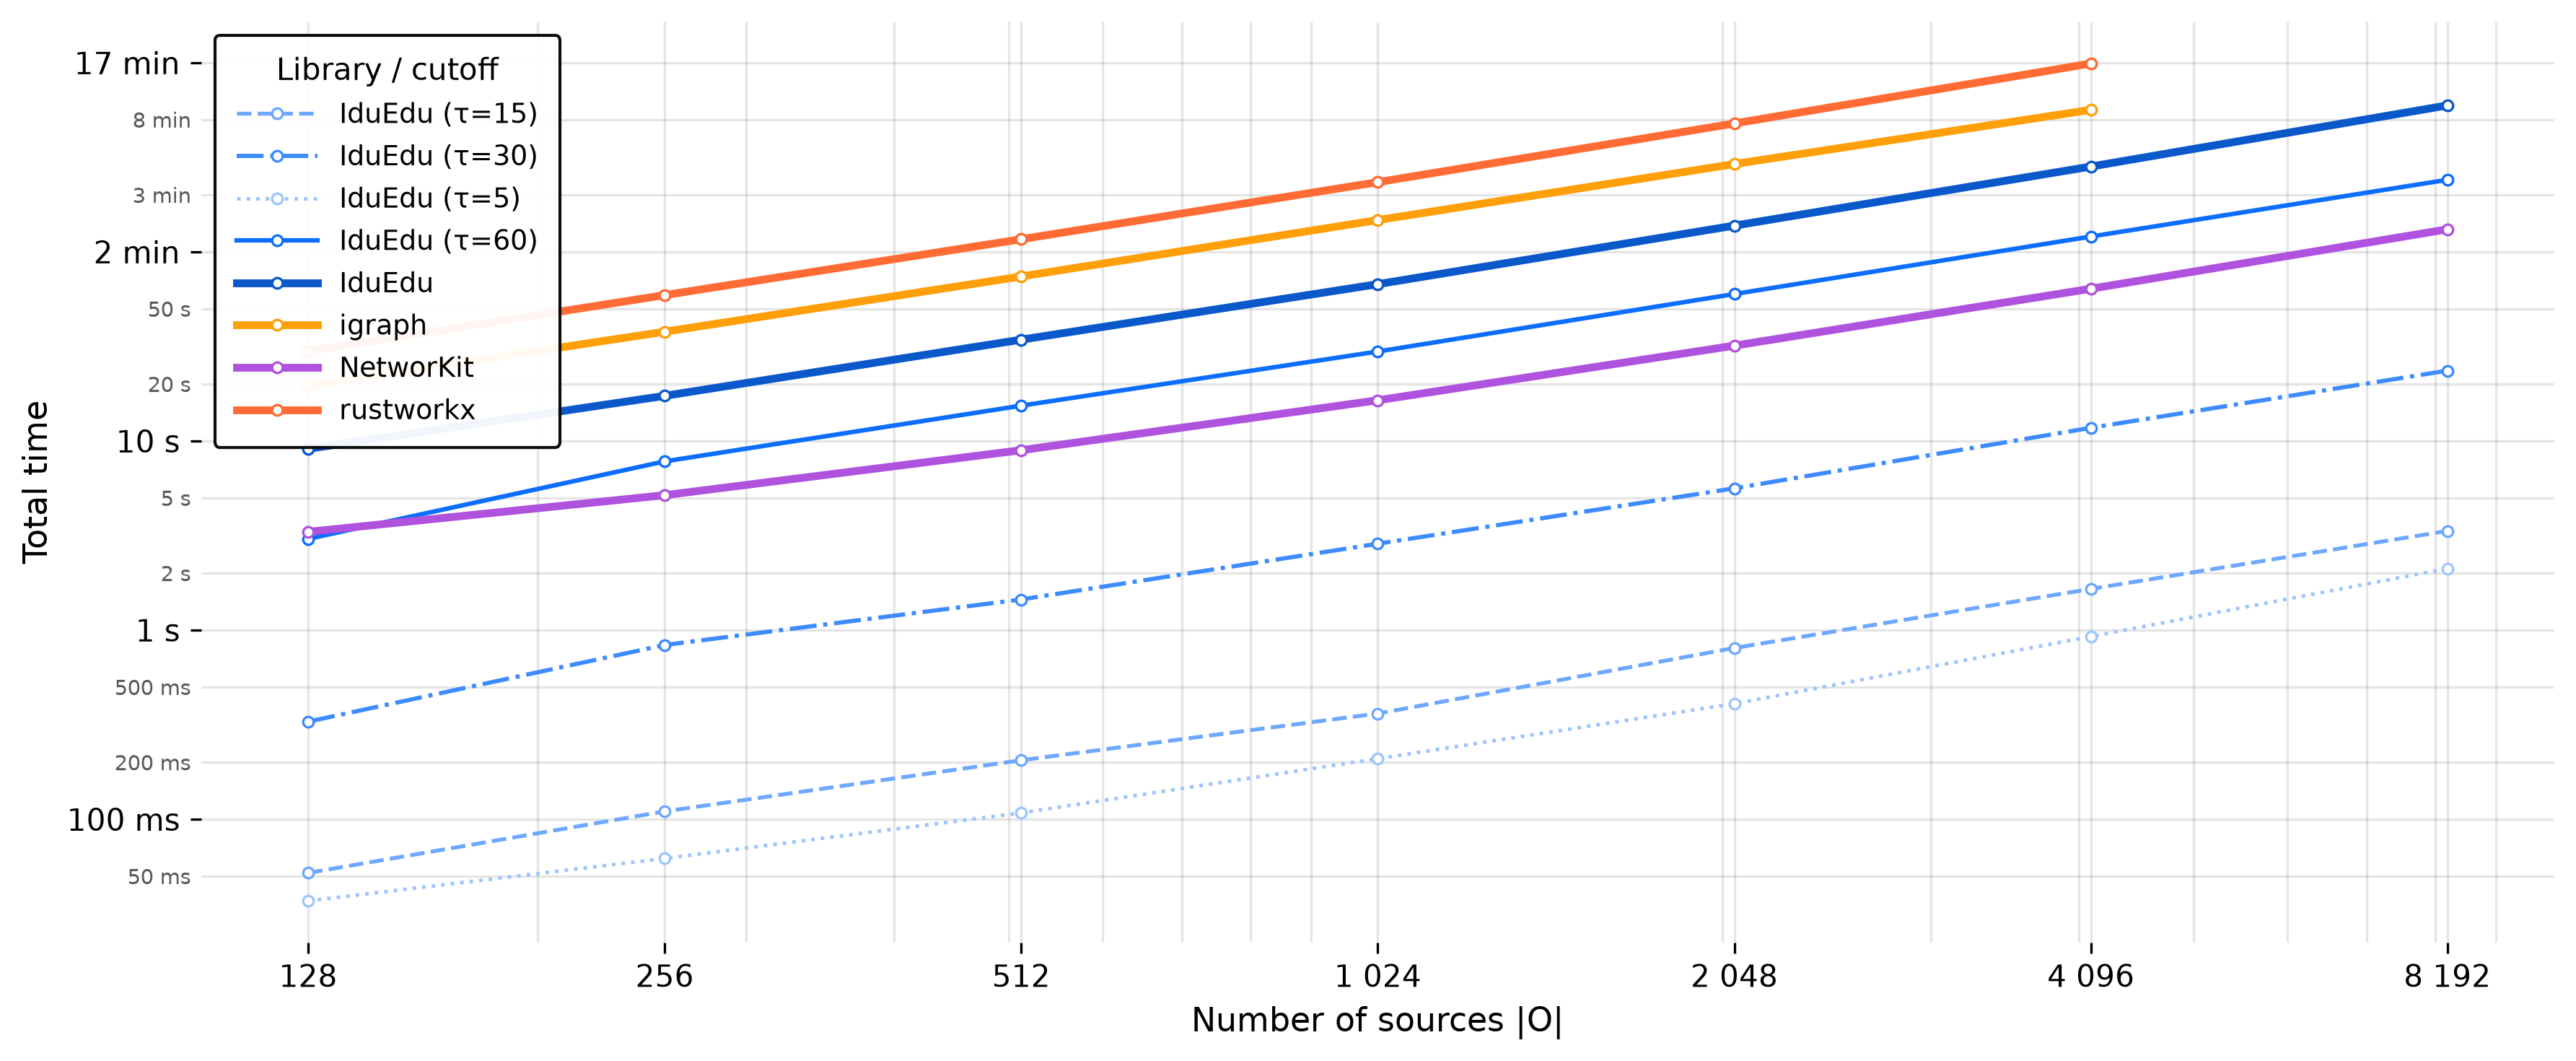
\includegraphics[width=\textwidth]{figures/od_time_square}
        \caption{Square OD computation time (origins $\to$ origins) for IduEdu, NetworKit and igraph, and
        the effect of the cutoff threshold on scalability.\label{fig:od_square}}
    \end{figure}

    \subsection{Ablation Studies}
    \label{subsec:res-ablations}

    The ablations isolate the contribution of three design decisions: street graph simplification, the
    OD cutoff, and adaptive graph reversal.

    \subsubsection{Graph Simplification}
    \label{subsubsec:abl-simplify}

    Simplification removes intermediate vertices and merges collinear edge sequences without changing
    topology or losing geometric information.
    The ablation compares IduEdu build time with simplification on and off, recording median build
    time, resulting edge count and deterministic memory of the graph tables per city.
    As Figure~\ref{fig:ablation_simplify} shows, the effect is not universal but topology-dependent.
    In walk networks, the dense structure of intersections and local geometric joints makes
    spatial merging expensive: such graphs build faster without simplification, yet the simplified
    graph remains far more compact---simplification cuts edge count and memory by
    ${\approx}2$--$3\times$.
    For drive networks, with longer linear stretches and fewer micro-intersections, merging pays off
    already at build time, reducing both edges and build time.
    Simplification is therefore a topology-dependent trade between geometric merge cost and output
    size: worthwhile preparation whenever heavy downstream computation follows
    (Section~\ref{subsec:res-od}), and reasonably skipped for one-off builds.

    \begin{figure}[H]
        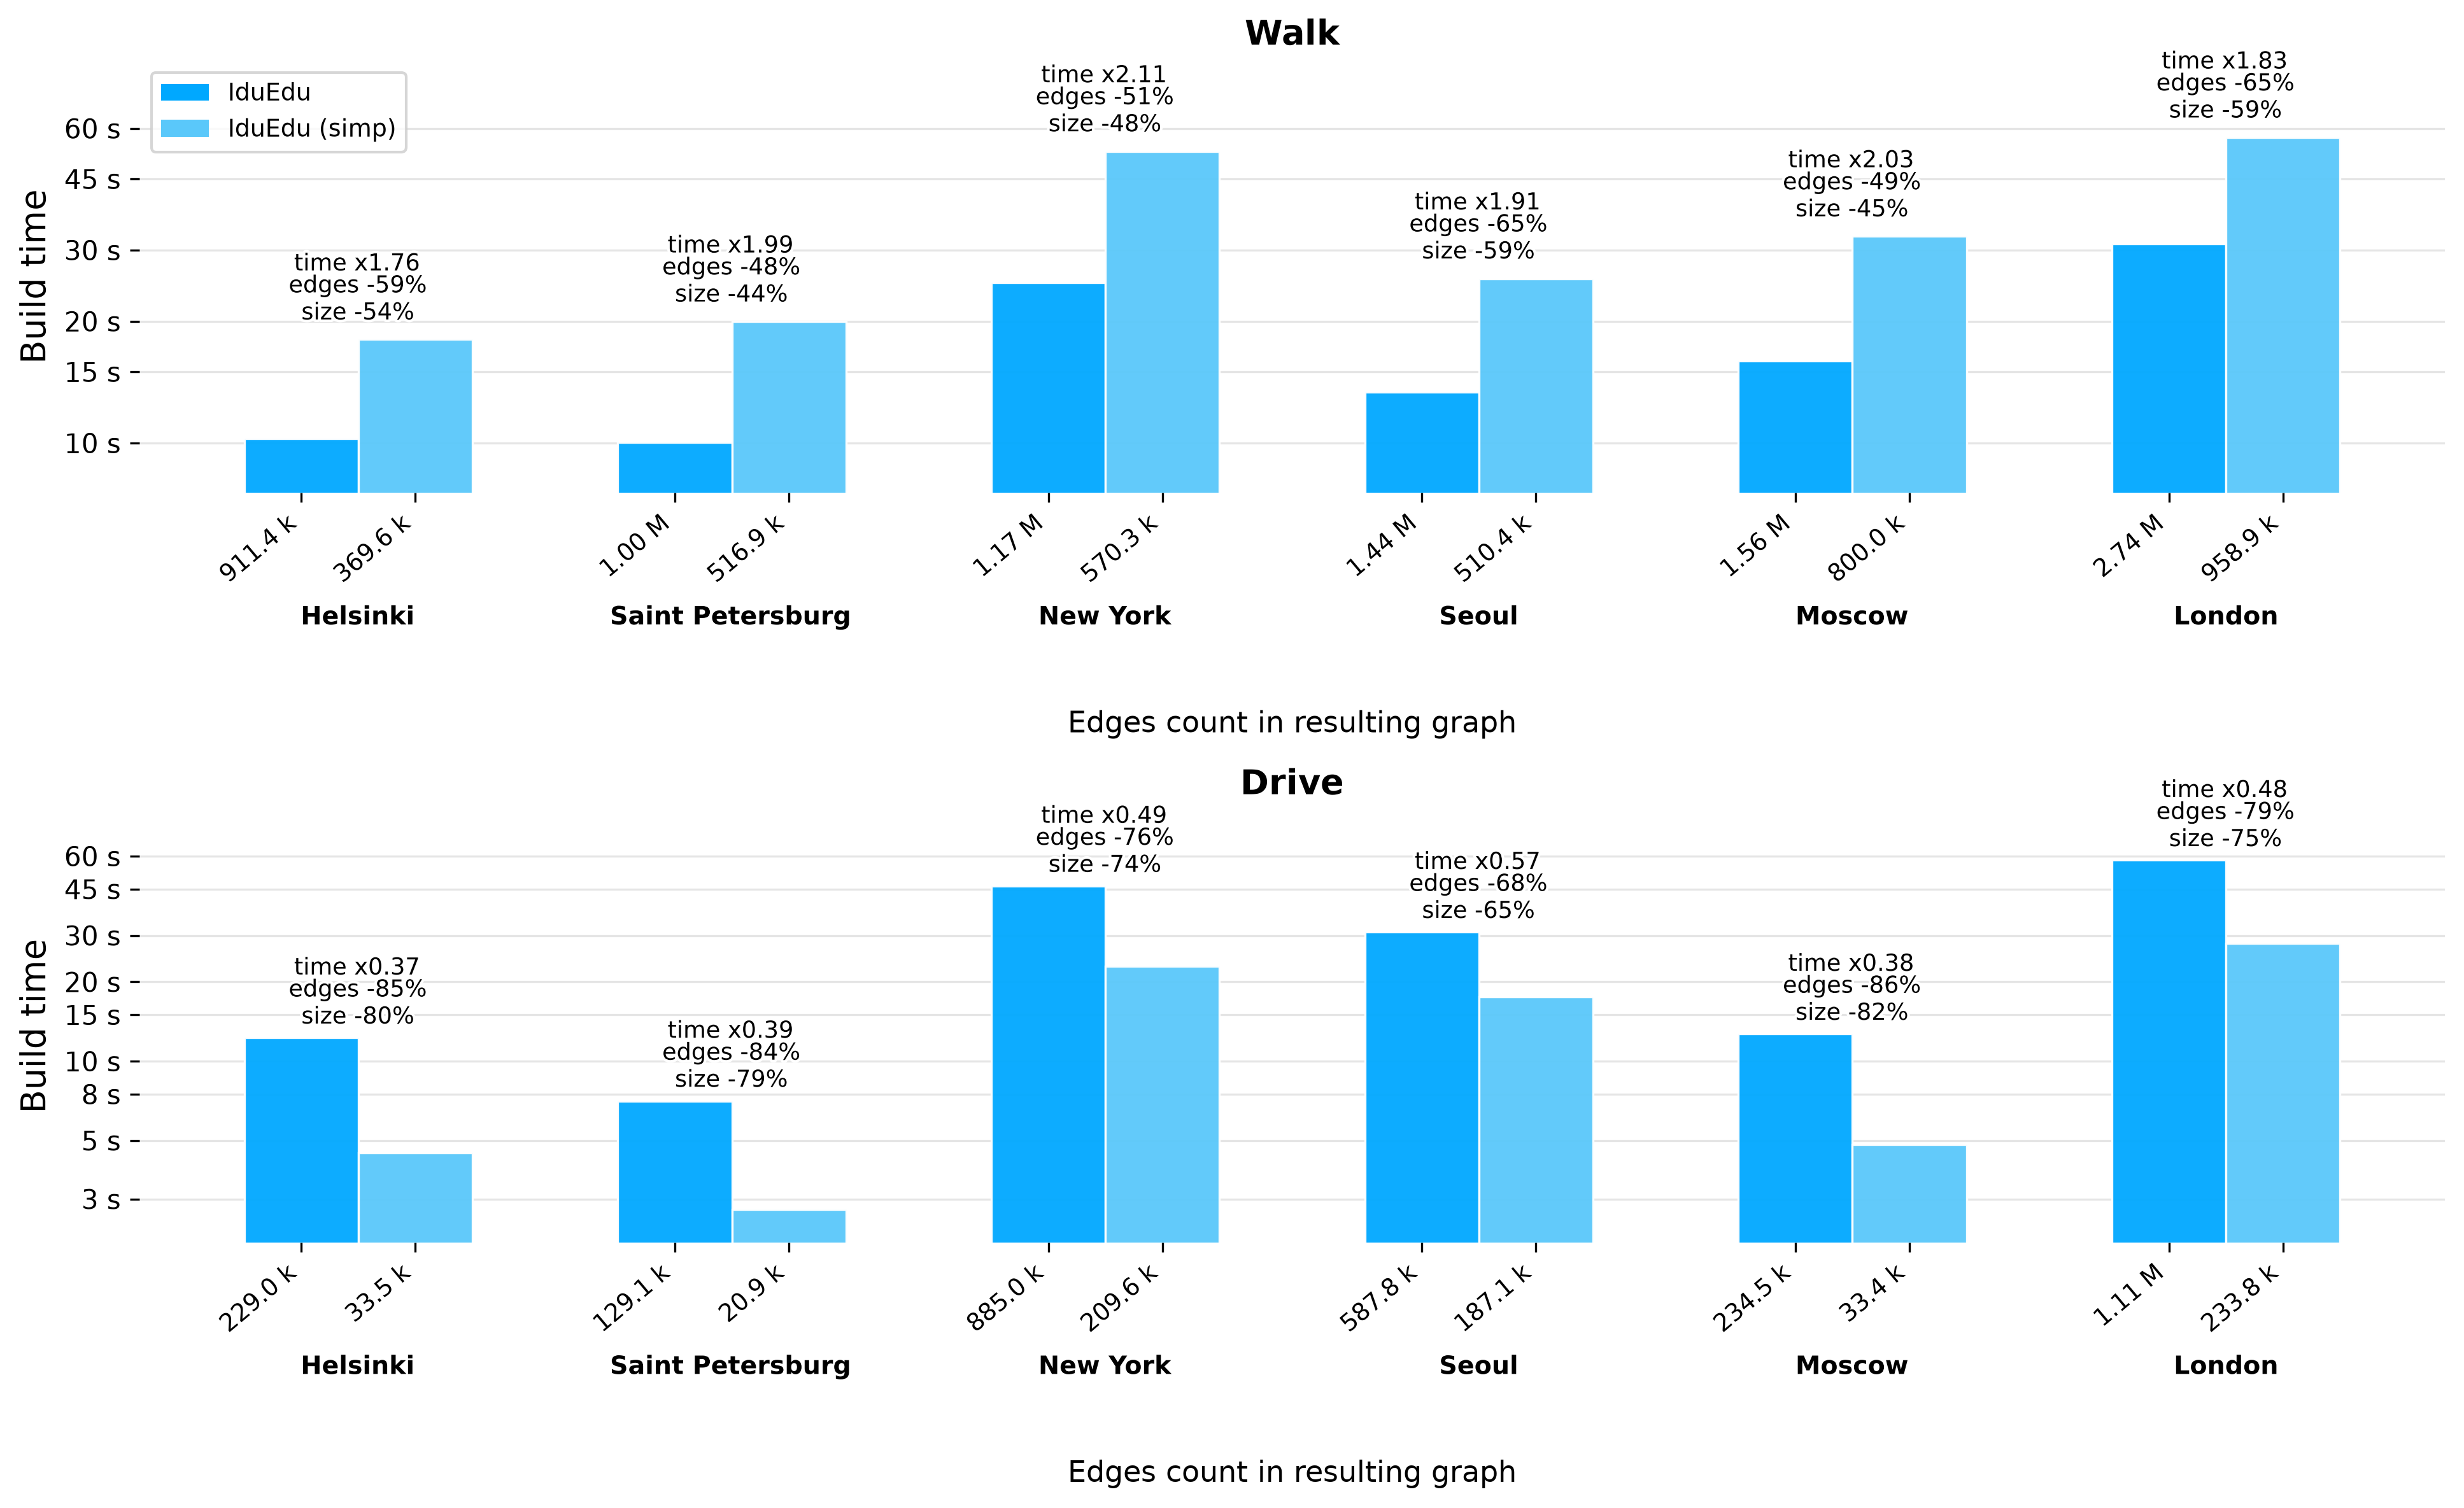
\includegraphics[width=\textwidth]{figures/ablation_simplify}
        \caption{Effect of graph simplification on build time for walk and drive networks in IduEdu.
        Bars are annotated with resulting edge counts; group annotations give the relative change in build
        time, edge count and memory when simplification is enabled.\label{fig:ablation_simplify}}
    \end{figure}

    \subsubsection{Cutoff in OD Computation}
    \label{subsubsec:abl-cutoff}

    This ablation is internal to IduEdu: for square OD matrices it compares the library's own full
    computation against its bounded variant at several path-time thresholds $\tau$---an ablation of the
    mechanism, not a cross-library comparison.
    The cutoff intentionally returns a sparse local-reachability matrix; a high share of unreached
    pairs indicates pairs beyond the specified time radius, not missing results, and directly explains
    the localization of the search.
    As Table~\ref{tab:cutoff} shows, savings grow with matrix size and shrink with the threshold: at
    $\tau = 5$~min and $|O| = 8{,}192$ the speedup over full computation reaches ${\approx}259\times$,
    while at $\tau = 60$~min it declines to ${\approx}2\times$ as the bounded search approaches a full
    traversal.
    Cutoff is thus most effective precisely in the local-accessibility scenarios typical of walk and
    PT analysis.

    \begin{table}[H]
        \caption{Relative speed-up of OD matrix computation in IduEdu with cutoff $\tau$ for square OD
        matrices ($|O| = |D|$), measured against IduEdu's own full computation without
        cutoff.\label{tab:cutoff}}
        \begin{tabularx}{\textwidth}{lCCCCCCC}
            \toprule
            $\tau$ (min) & \textbf{128} & \textbf{256} & \textbf{512} & \textbf{1024} & \textbf{2048} & \textbf{4096} & \textbf{8192}\\
            \midrule
            5            & 237.9        & 240.3        & 290.2        & 261.0         & 254.3         & 247.3         & 258.9         \\
            15           & 160.2        & 132.8        & 135.4        & 157.5         & 153.6         & 157.7         & 163.6         \\
            30           & 25.6         & 17.8         & 17.6         & 22.2          & 21.8          & 21.3          & 23.3          \\
            60           & 2.7          & 2.1          & 2.2          & 2.2           & 2.3           & 2.3           & 2.4           \\
            \bottomrule
        \end{tabularx}
    \end{table}

    \subsubsection{Adaptive Graph Reversal}
    \label{subsubsec:abl-reversal}

    Adaptive reversal applies to rectangular OD matrices when origins outnumber destinations.
    Since one Dijkstra run covers all reachable vertices, an OD matrix between sets of cardinality
    $|O|$ and $|D|$ requires $\min(|O|, |D|)$ runs.
    The B3 results (Figure~\ref{fig:od_rect}) show that at $|O| \gg |D|$ reversal stabilizes IduEdu's
    computation time: as $|O|$ grows at fixed $|D| = 911$, the number of runs is pinned to $|D|$ and the
    time curve flattens to a plateau, whereas NetworKit and igraph, lacking reversal, scale their run
    count with $|O|$.
    By construction the effect vanishes for square matrices (Figure~\ref{fig:od_square}), but it is
    decisive in the rectangular settings typical of accessibility assessment.

    \subsection{Table-First Workflow, Graph Reuse and Their Cost}
    \label{subsec:res-workflow}

    Before turning to the applied results, we quantify what it costs to operate the pipeline, since
    this is what makes the repeated analyses of Sections~\ref{subsec:res-p1}
    and~\ref{subsec:res-p0} practical at all.

    A scenario is an ordinary edit of the edge table (Listing~\ref{lst:tablefirst},
    Figure~\ref{fig:tablefirst}).
    Locating and editing boarding edges by an attribute mask takes milliseconds (0.001--0.08~s for
    55--1{,}823 edges); rebuilding the cached CSR of the 776{,}051-edge multimodal graph takes
    ${\approx}1.3$~s; and re-running nearest-school and school-count routing for all 83{,}510 origins
    takes ${\approx}5$--$7$~s.
    A complete city-scale what-if evaluation is thus a ${\approx}7$-second operation, and ObjectNat
    consumes the modified \texttt{UrbanGraph} directly to rebuild polygon products.

    The graph itself is built once and reused.
    Table~\ref{tab:cache_timing} decomposes the end-to-end cost of the case study.
    Building the city multimodal graph from cached OSM responses takes 159.7~s and writing both
    \texttt{.urbangraph} files (with the CSR included) another 12.5~s---paid once; every later
    analysis starts from a 2.3~s warm load.
    ObjectNat polygon construction costs 10--106~s per operation---up to an order of magnitude above
    routing---which is why isochrone and coverage geometries are cached alongside the graphs.
    The first scenario of a session additionally pays JIT warm-up (17.3~s); all subsequent scenarios
    run at the 6.7~s median quoted above.

    \begin{figure}[H]
        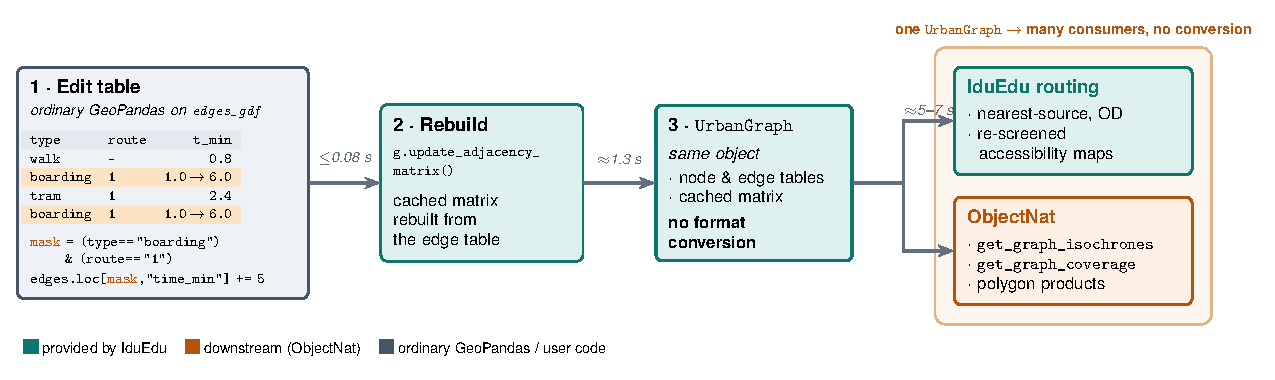
\includegraphics[width=\textwidth]{figures/tablefirst_figure}
        \caption{Table-first extensibility and ObjectNat integration. A scenario is expressed as an
        ordinary GeoPandas mask over the \texttt{edges\_gdf} table and an assignment to a cost column
            (here, a waiting penalty on the boarding edges of one route); the cached computational form is
            rebuilt in place with \texttt{update\_adjacency\_matrix}, and the \emph{same}
            \texttt{UrbanGraph} object then feeds both IduEdu's routing primitives and the downstream
            ObjectNat isochrone/coverage functions without any format conversion. Approximate wall-clock
            costs at city scale (776{,}051-edge graph, 83{,}510 origins) annotate the
            arrows.\label{fig:tablefirst}}
    \end{figure}

    \begin{table}[H]
        \caption{End-to-end timing of the city-scale case study (single workstation).\label{tab:cache_timing}}
        \begin{tabularx}{\textwidth}{lCC}
            \toprule
            \textbf{Stage}                                        & \textbf{Cold, s}  & \textbf{Warm, s}       \\
            \midrule
            Multimodal graph build (from cached OSM data)         & 159.7             & ---                    \\
            Graph write / load (\texttt{.urbangraph}, incl.\ CSR) & 12.5              & 2.3                    \\
            Snap + nearest-school routing (per network)           & ---               & 1.4--1.7               \\
            School-count OD, 83{,}510 $\times$ 911                & ---               & 6.1 (walk) / 38.0 (mm) \\
            Scenario pass (edit + CSR rebuild + routing)          & 17.3 (first, JIT) & 6.7 (median)           \\
            ObjectNat polygon construction                        & ---               & 10--106 per operation  \\
            \bottomrule
        \end{tabularx}
    \end{table}

    \subsection{School Accessibility in Saint Petersburg: Walk vs.\ Multimodal}
    \label{subsec:res-case}

    Table~\ref{tab:reachable_schools} summarizes the baseline, and two features stand out.
    First, the time to the \emph{nearest} school barely changes when PT is added: the median is
    10.5~min on the walk network and 10.3~min on the multimodal one.
    In a city where the nearest school is typically a short walk away, PT is not needed for first
    access; its effect appears in the tail of the distribution (90th percentile: 33.4 vs.\ 26.1~min)
    and in peripheral pockets (Figure~\ref{fig:coverage}, right).
    Second, the number of reachable schools---the opportunity metric---responds strongly, and the
    response grows with the travel-time budget.
    At 15~min, PT adds almost nothing (+0.4 schools on average): short trips are dominated by walking
    once the modeled boarding cost is paid.
    At 30~min it multiplies the mean opportunity set by 2.5 (9.5 $\to$ 23.5 schools; median 4 $\to$ 7),
    at 45~min by 4.7 (19.2 $\to$ 90.3), and no saturation occurs even at 60~min.
    Figure~\ref{fig:isochrones} shows the mechanism behind these numbers for a single origin: within
    the same 30-min budget, the reachable area grows from one compact walking neighbourhood to a
    corridor-shaped region stretched along the transit network, which is what brings distant schools
    into range.
    Read methodologically, this is the answer to RQ4: an assessment built on the walk-only network that
    current extraction tools provide would describe basic school access correctly, but would understate
    the reachable opportunity set 2.5-fold at a 30-min budget and---as
    Section~\ref{subsec:res-p1} shows---would give no indication of how few routes that difference
    rests on.

    Coverage moves accordingly: the share of buildings with at least one school within 30~min rises
    from 88.0\% to 93.5\%, and within 45~min from 94.3\% to 98.0\%.
    The secondary population-weighted comparison is deliberately reported as a walk-to-multimodal
    difference rather than as an absolute coverage claim: the gain is 0.57 percentage points at
    15~min, 0.61 at 30~min, 0.39 at 45~min and 0.16 at 60~min.
    In this allocation, PT thus changes the coverage of residential locations more strongly than the
    share of assigned population; this relative result is not interpreted as an equity measure.

    Figure~\ref{fig:gain_metrics} details the distribution of the gain: at the 30-min budget, 71.0\%
    of residential buildings gain at least one school, 17.6\% gain 6--20, and 8.2\% gain more than 50.
    The 15-min classification of Section~\ref{subsec:indicators} localizes the effect spatially
    (Figure~\ref{fig:gain_map}): 48.6\% of buildings see no effect and a further 33.7\% reach no
    school within 15~min on either network, while the substantial (9.7\%), moderate (5.6\%) and newly
    reachable (2.5\%) classes concentrate along tram and subway corridors.
    The computation behind these results is fast: snapping and nearest-school routing take
    1.4--1.7~s per network, and the complete 83{,}510$\times$911 school-count computation takes 6.1~s
    on the walk graph and 38.0~s on the multimodal graph.

    \begin{table}[H]
        \caption{Number of schools reachable per residential origin within each travel-time cutoff, on
        the walk and multimodal networks (83{,}510 residential origins, 911 schools). All values are
        counts of schools; \emph{Gain} is the mean multimodal advantage over
        walking.\label{tab:reachable_schools}}
        \begin{tabularx}{\textwidth}{lCCCCC}
            \toprule
            & \multicolumn{3}{c}{\textbf{Mean (schools)}} & \multicolumn{2}{c}{\textbf{Median (schools)}} \\
            \cmidrule(lr){2-4}\cmidrule(lr){5-6}
            \textbf{Cutoff} & \textbf{Walk} & \textbf{Multimodal} & \textbf{Gain} & \textbf{Walk} & \textbf{Multimodal} \\
            \midrule
            15 min          & 2.78          & 3.16                & $+0.38$       & 1             & 1                   \\
            30 min          & 9.46          & 23.51               & $+14.05$      & 4             & 7                   \\
            45 min          & 19.18         & 90.32               & $+71.14$      & 8             & 21                  \\
            60 min          & 31.94         & 194.72              & $+162.79$     & 13            & 55                  \\
            \bottomrule
        \end{tabularx}
    \end{table}

    \begin{figure}[H]
        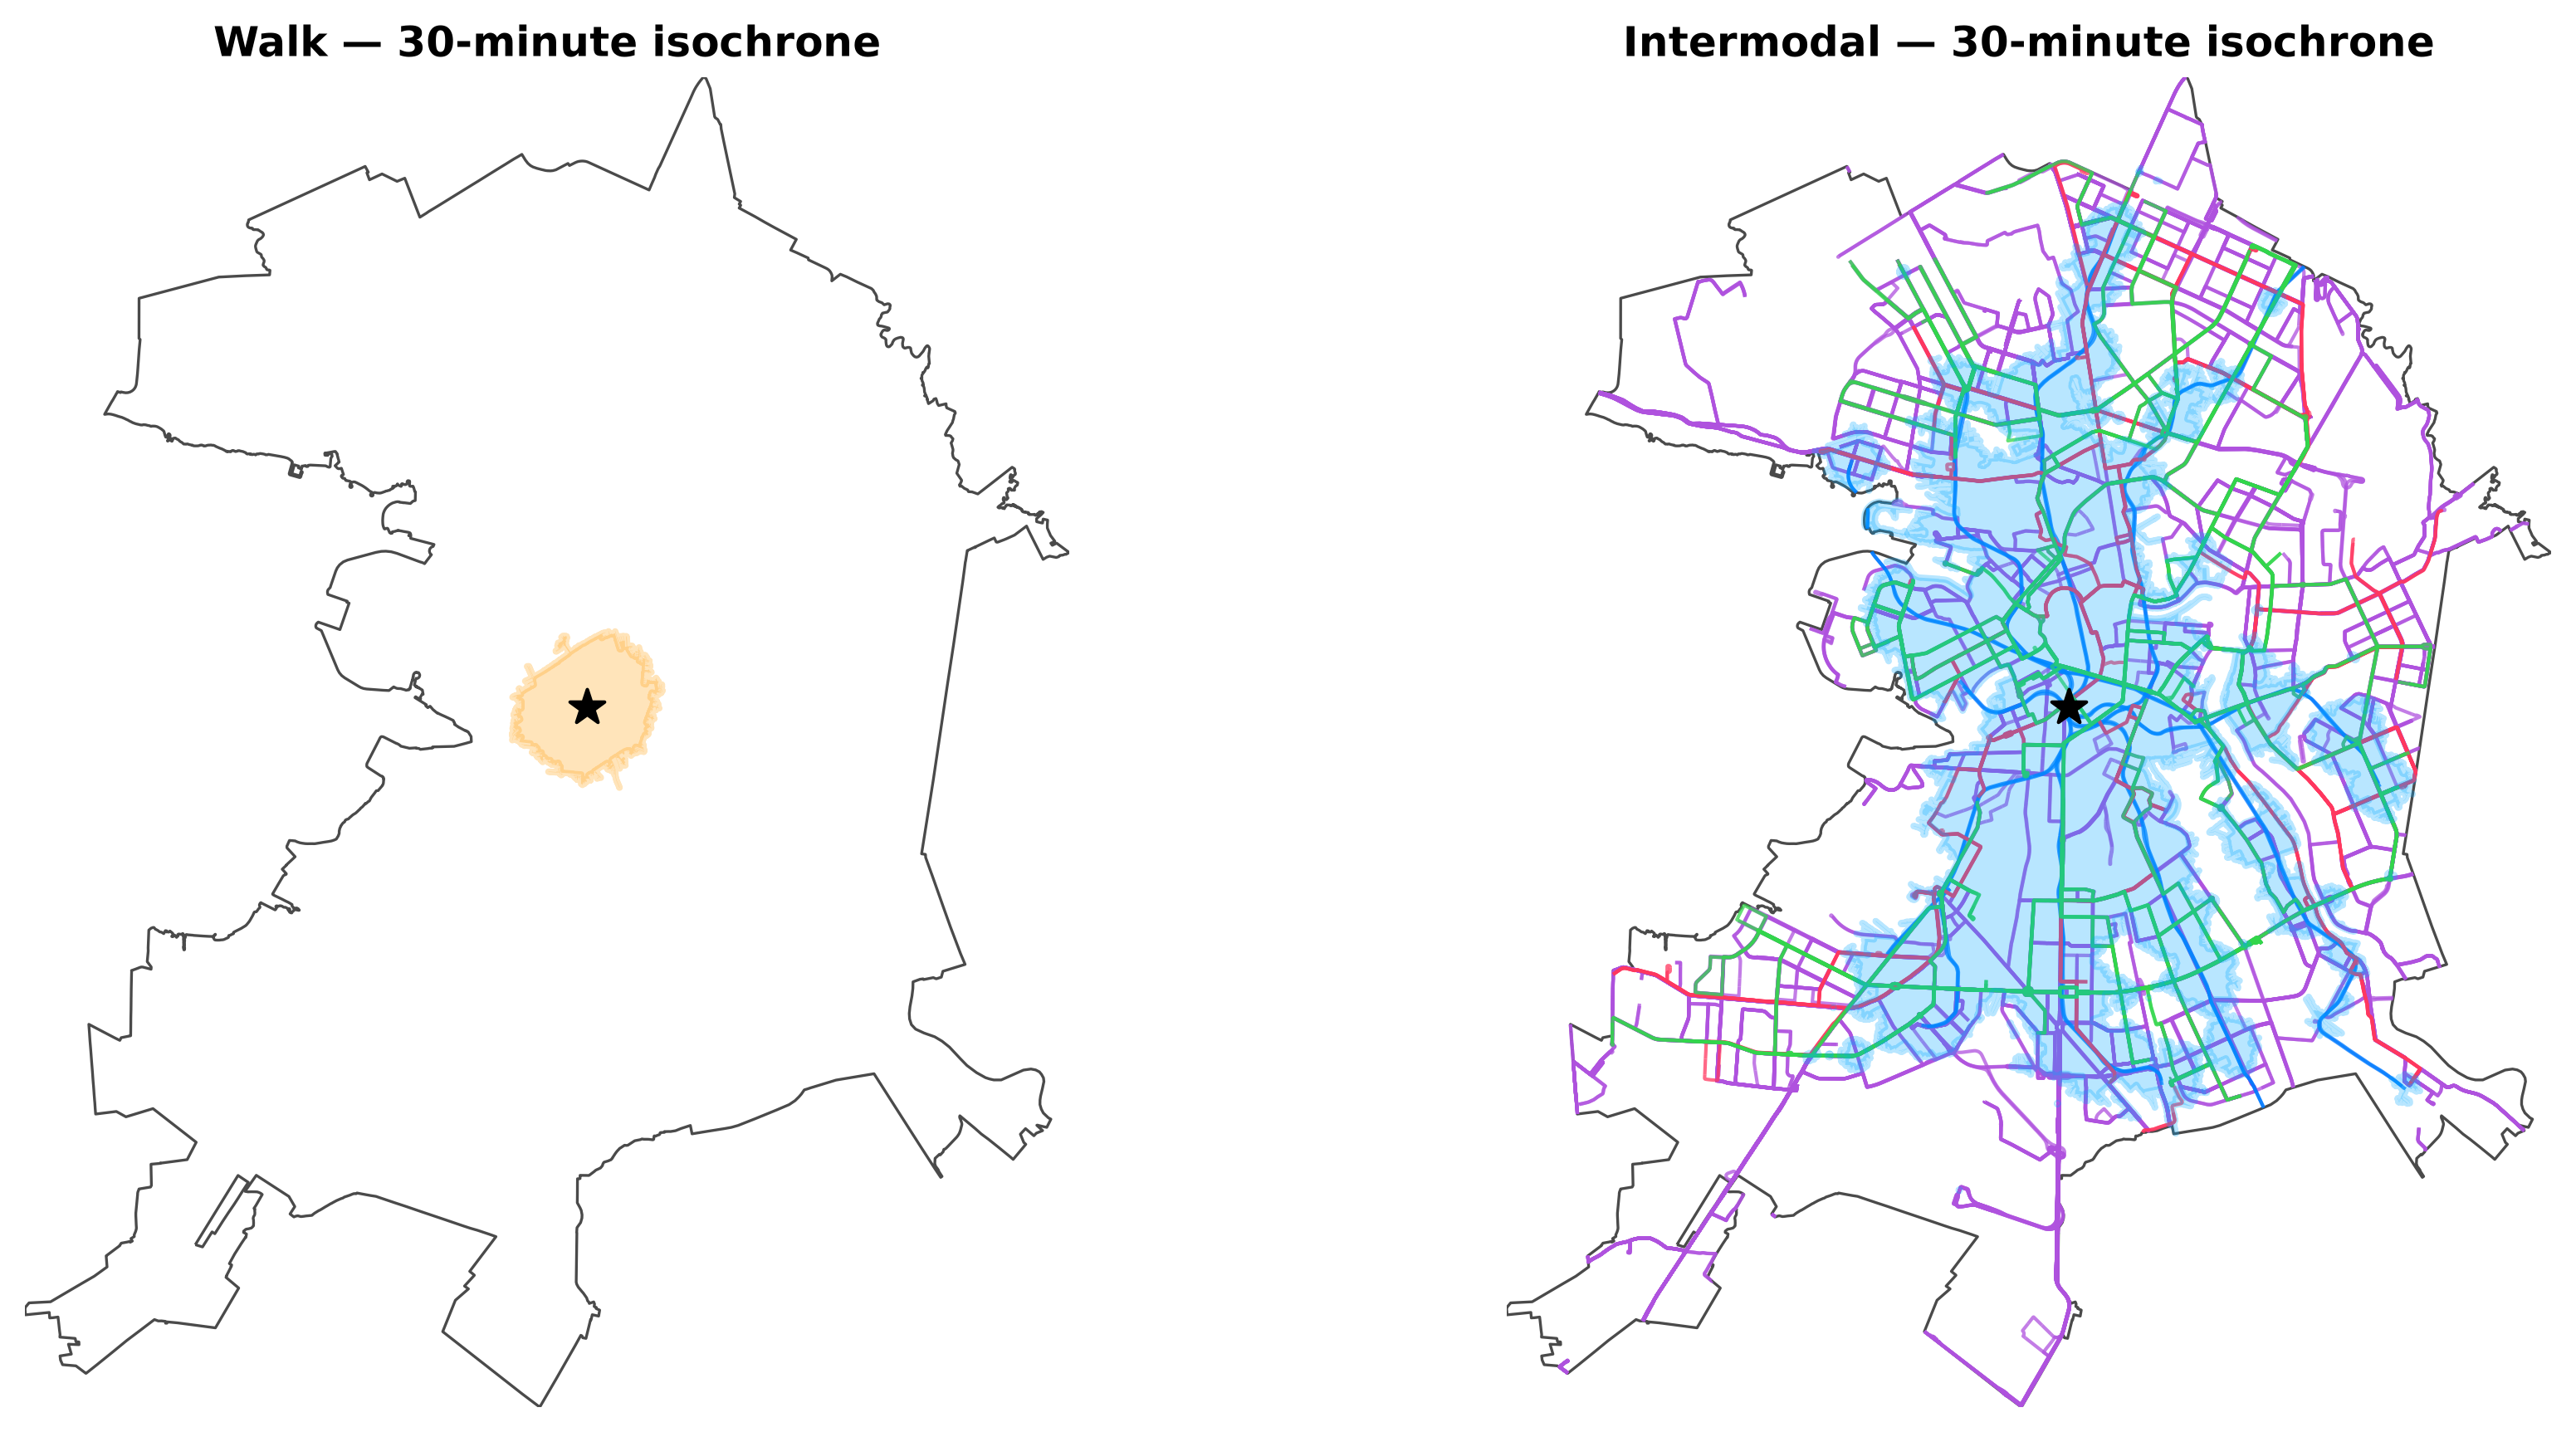
\includegraphics[width=\textwidth]{figures/objectnat_isochrone_comparison}
        \caption{Thirty-minute isochrones from the same central residential origin (black star), built
        with ObjectNat from the same \texttt{UrbanGraph} objects.
            (\textbf{Left}) Walk network; the reachable area is shown in orange.
            (\textbf{Right}) Multimodal network; the reachable area is shown in blue, with public
            transport routes drawn over it and colored by mode.
            Both panels share the same map extent, the outline being the historical city
            boundary.\label{fig:isochrones}}
    \end{figure}

    \begin{figure}[H]
        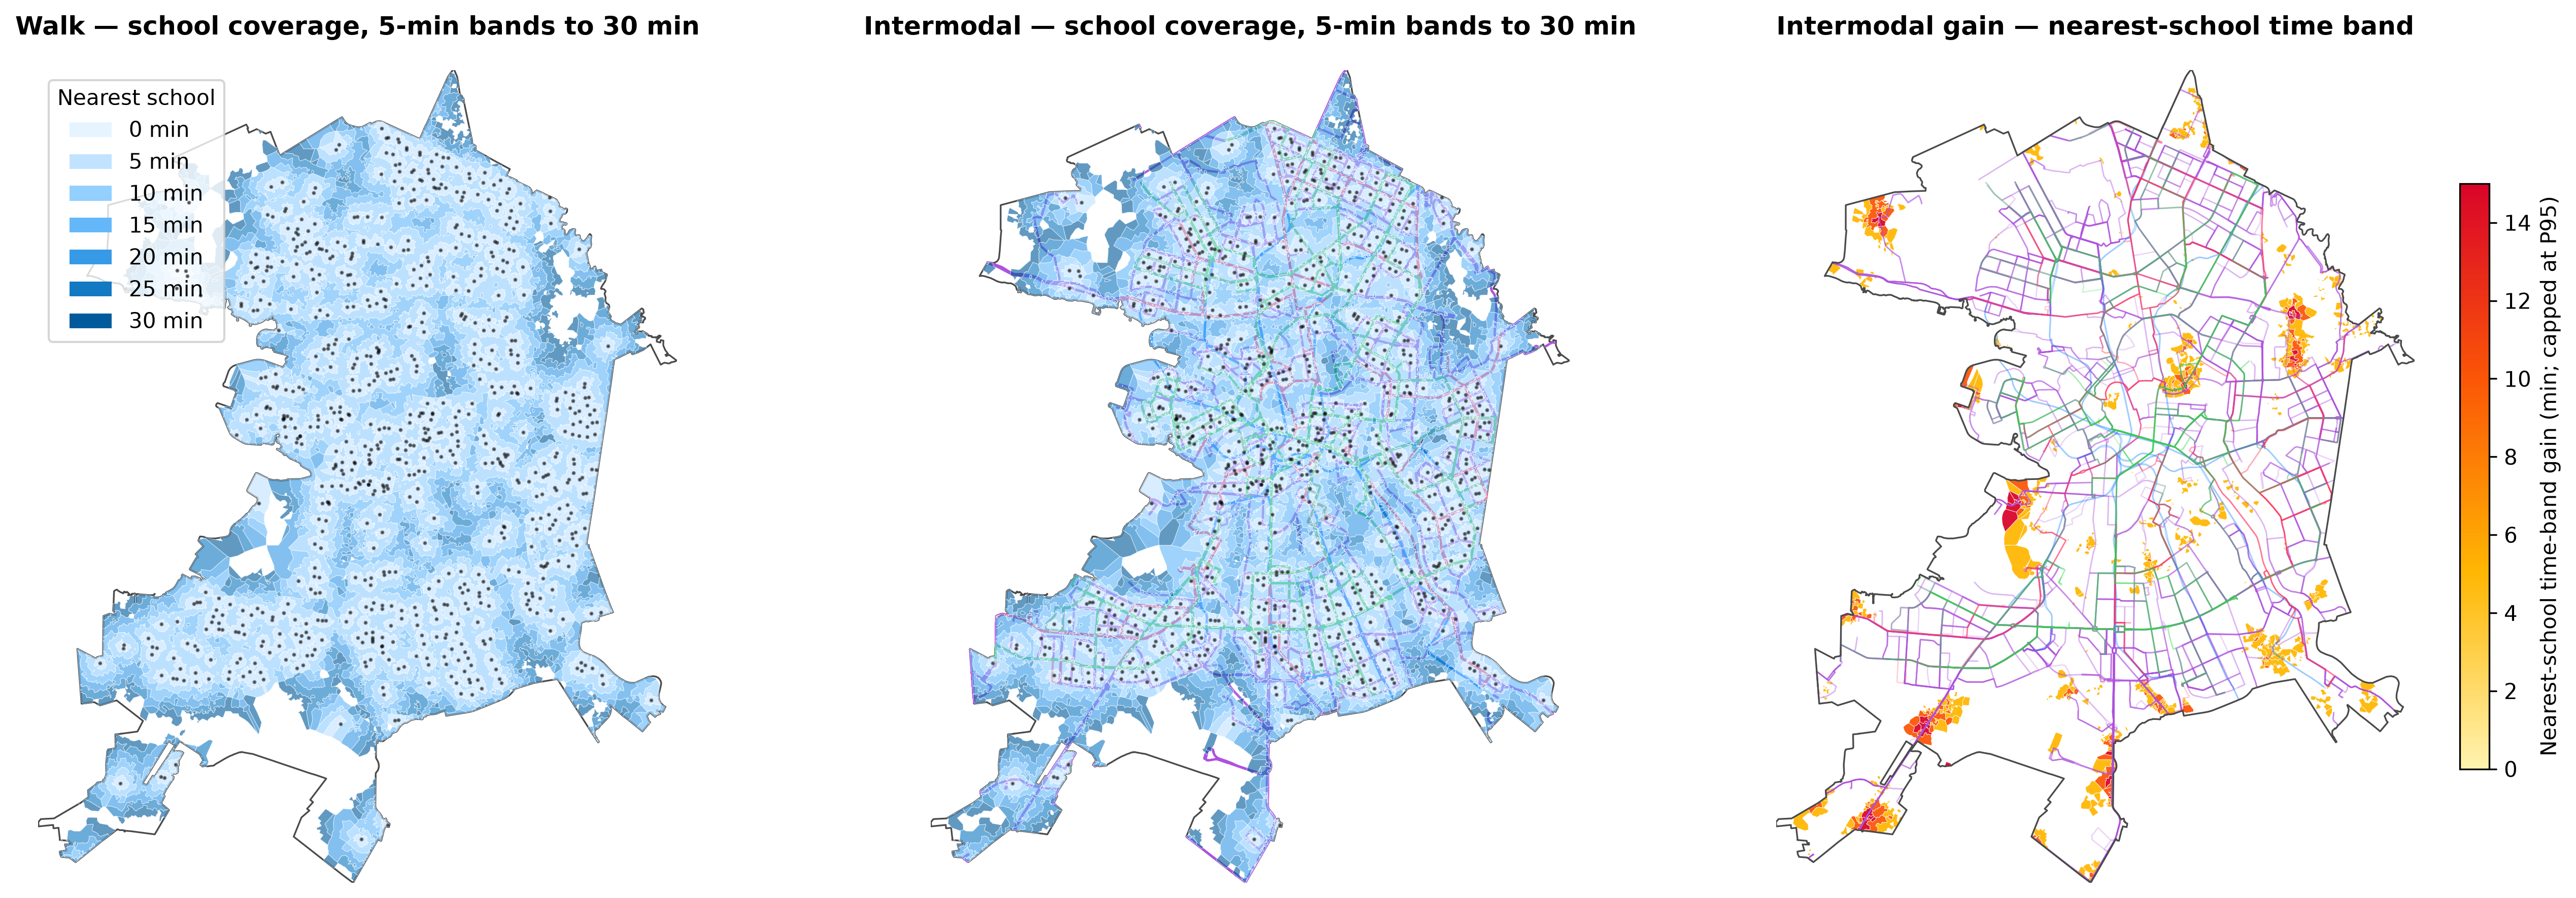
\includegraphics[width=\textwidth]{figures/objectnat_school_coverage}
        \caption{School coverage in 5-min bands up to 30 min on the walk (\textbf{left}) and multimodal
            (\textbf{center}) networks (ObjectNat reverse-search coverage; dots are schools).
            (\textbf{Right}) Nearest-school time-band gain of the multimodal network, highlighting the
            peripheral pockets where PT shortens first access.\label{fig:coverage}}
    \end{figure}

    \begin{figure}[H]
        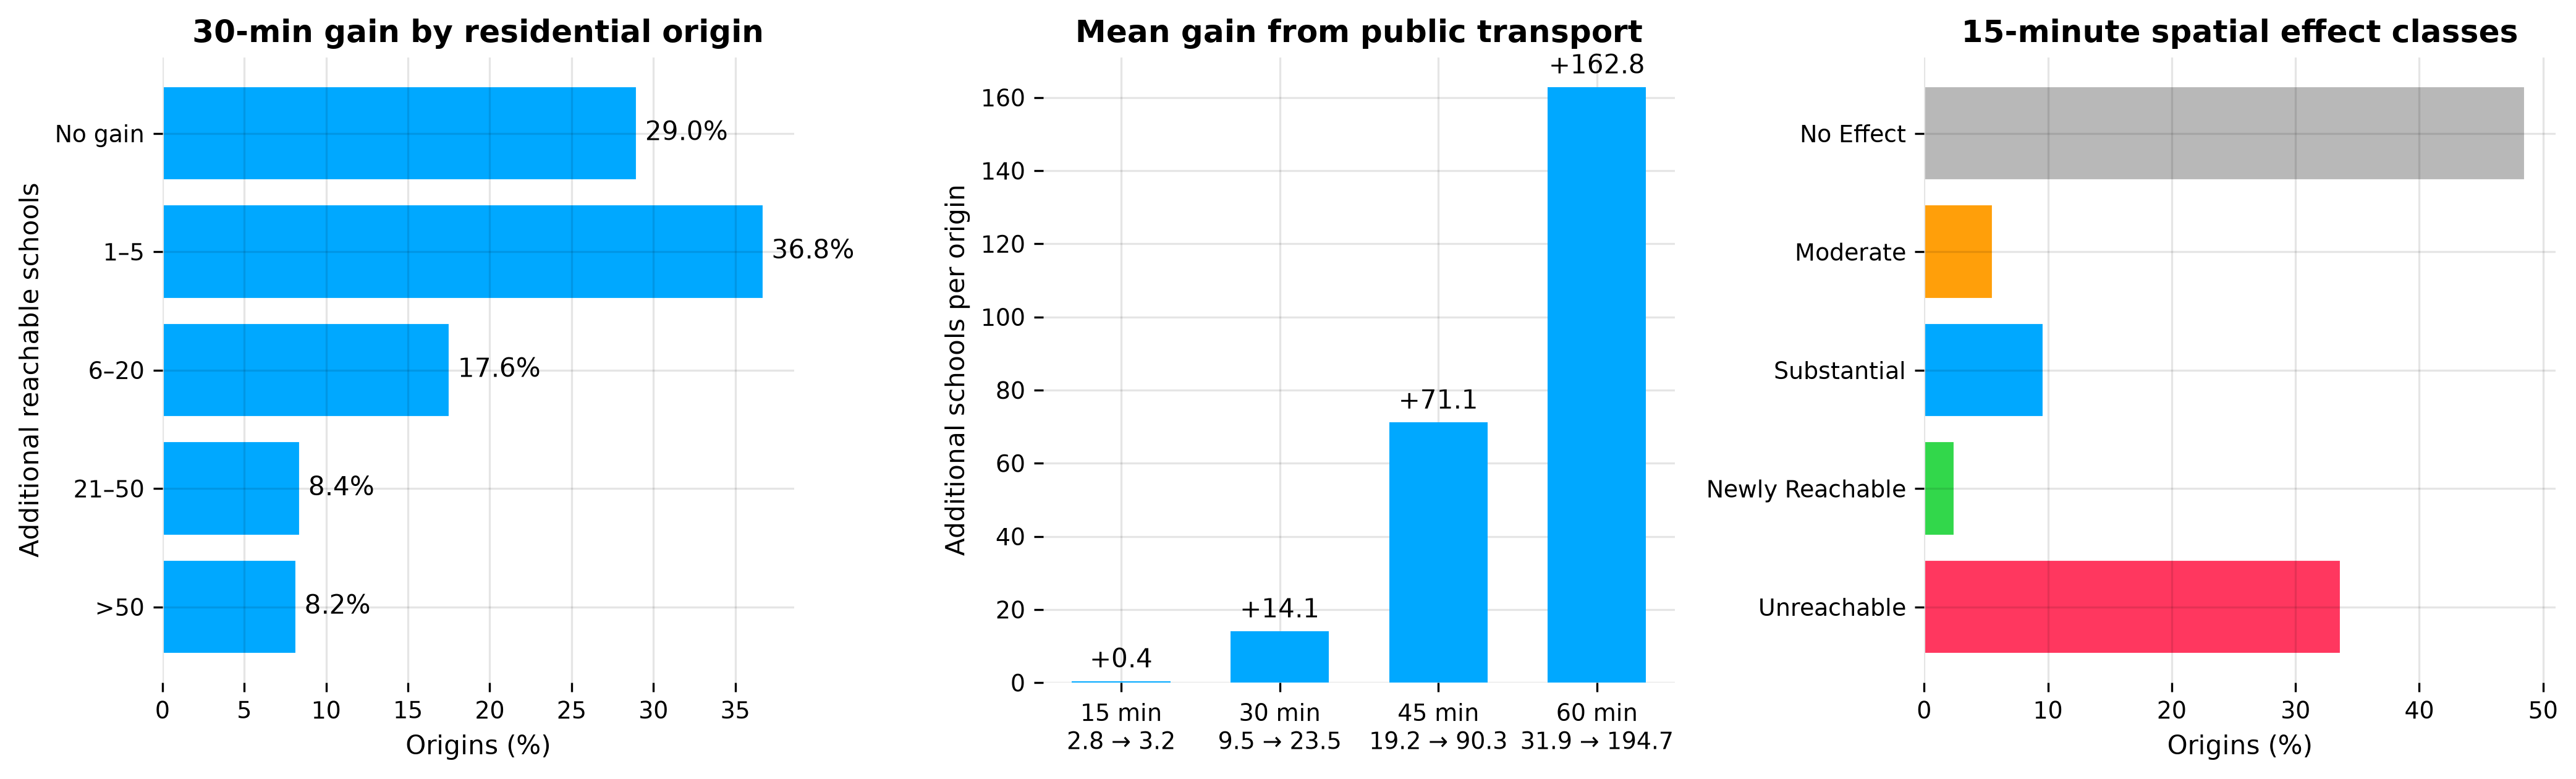
\includegraphics[width=\textwidth]{figures/accessibility_gain_metrics}
        \caption{Opportunity gain from public transport.
            (\textbf{Left}) Distribution of additional 30-min schools per residential origin.
            (\textbf{Center}) Mean reachable schools by cutoff, walk $\to$ multimodal.
            (\textbf{Right}) 15-min spatial effect classes.\label{fig:gain_metrics}}
    \end{figure}

    \begin{figure}[H]
        \centering
        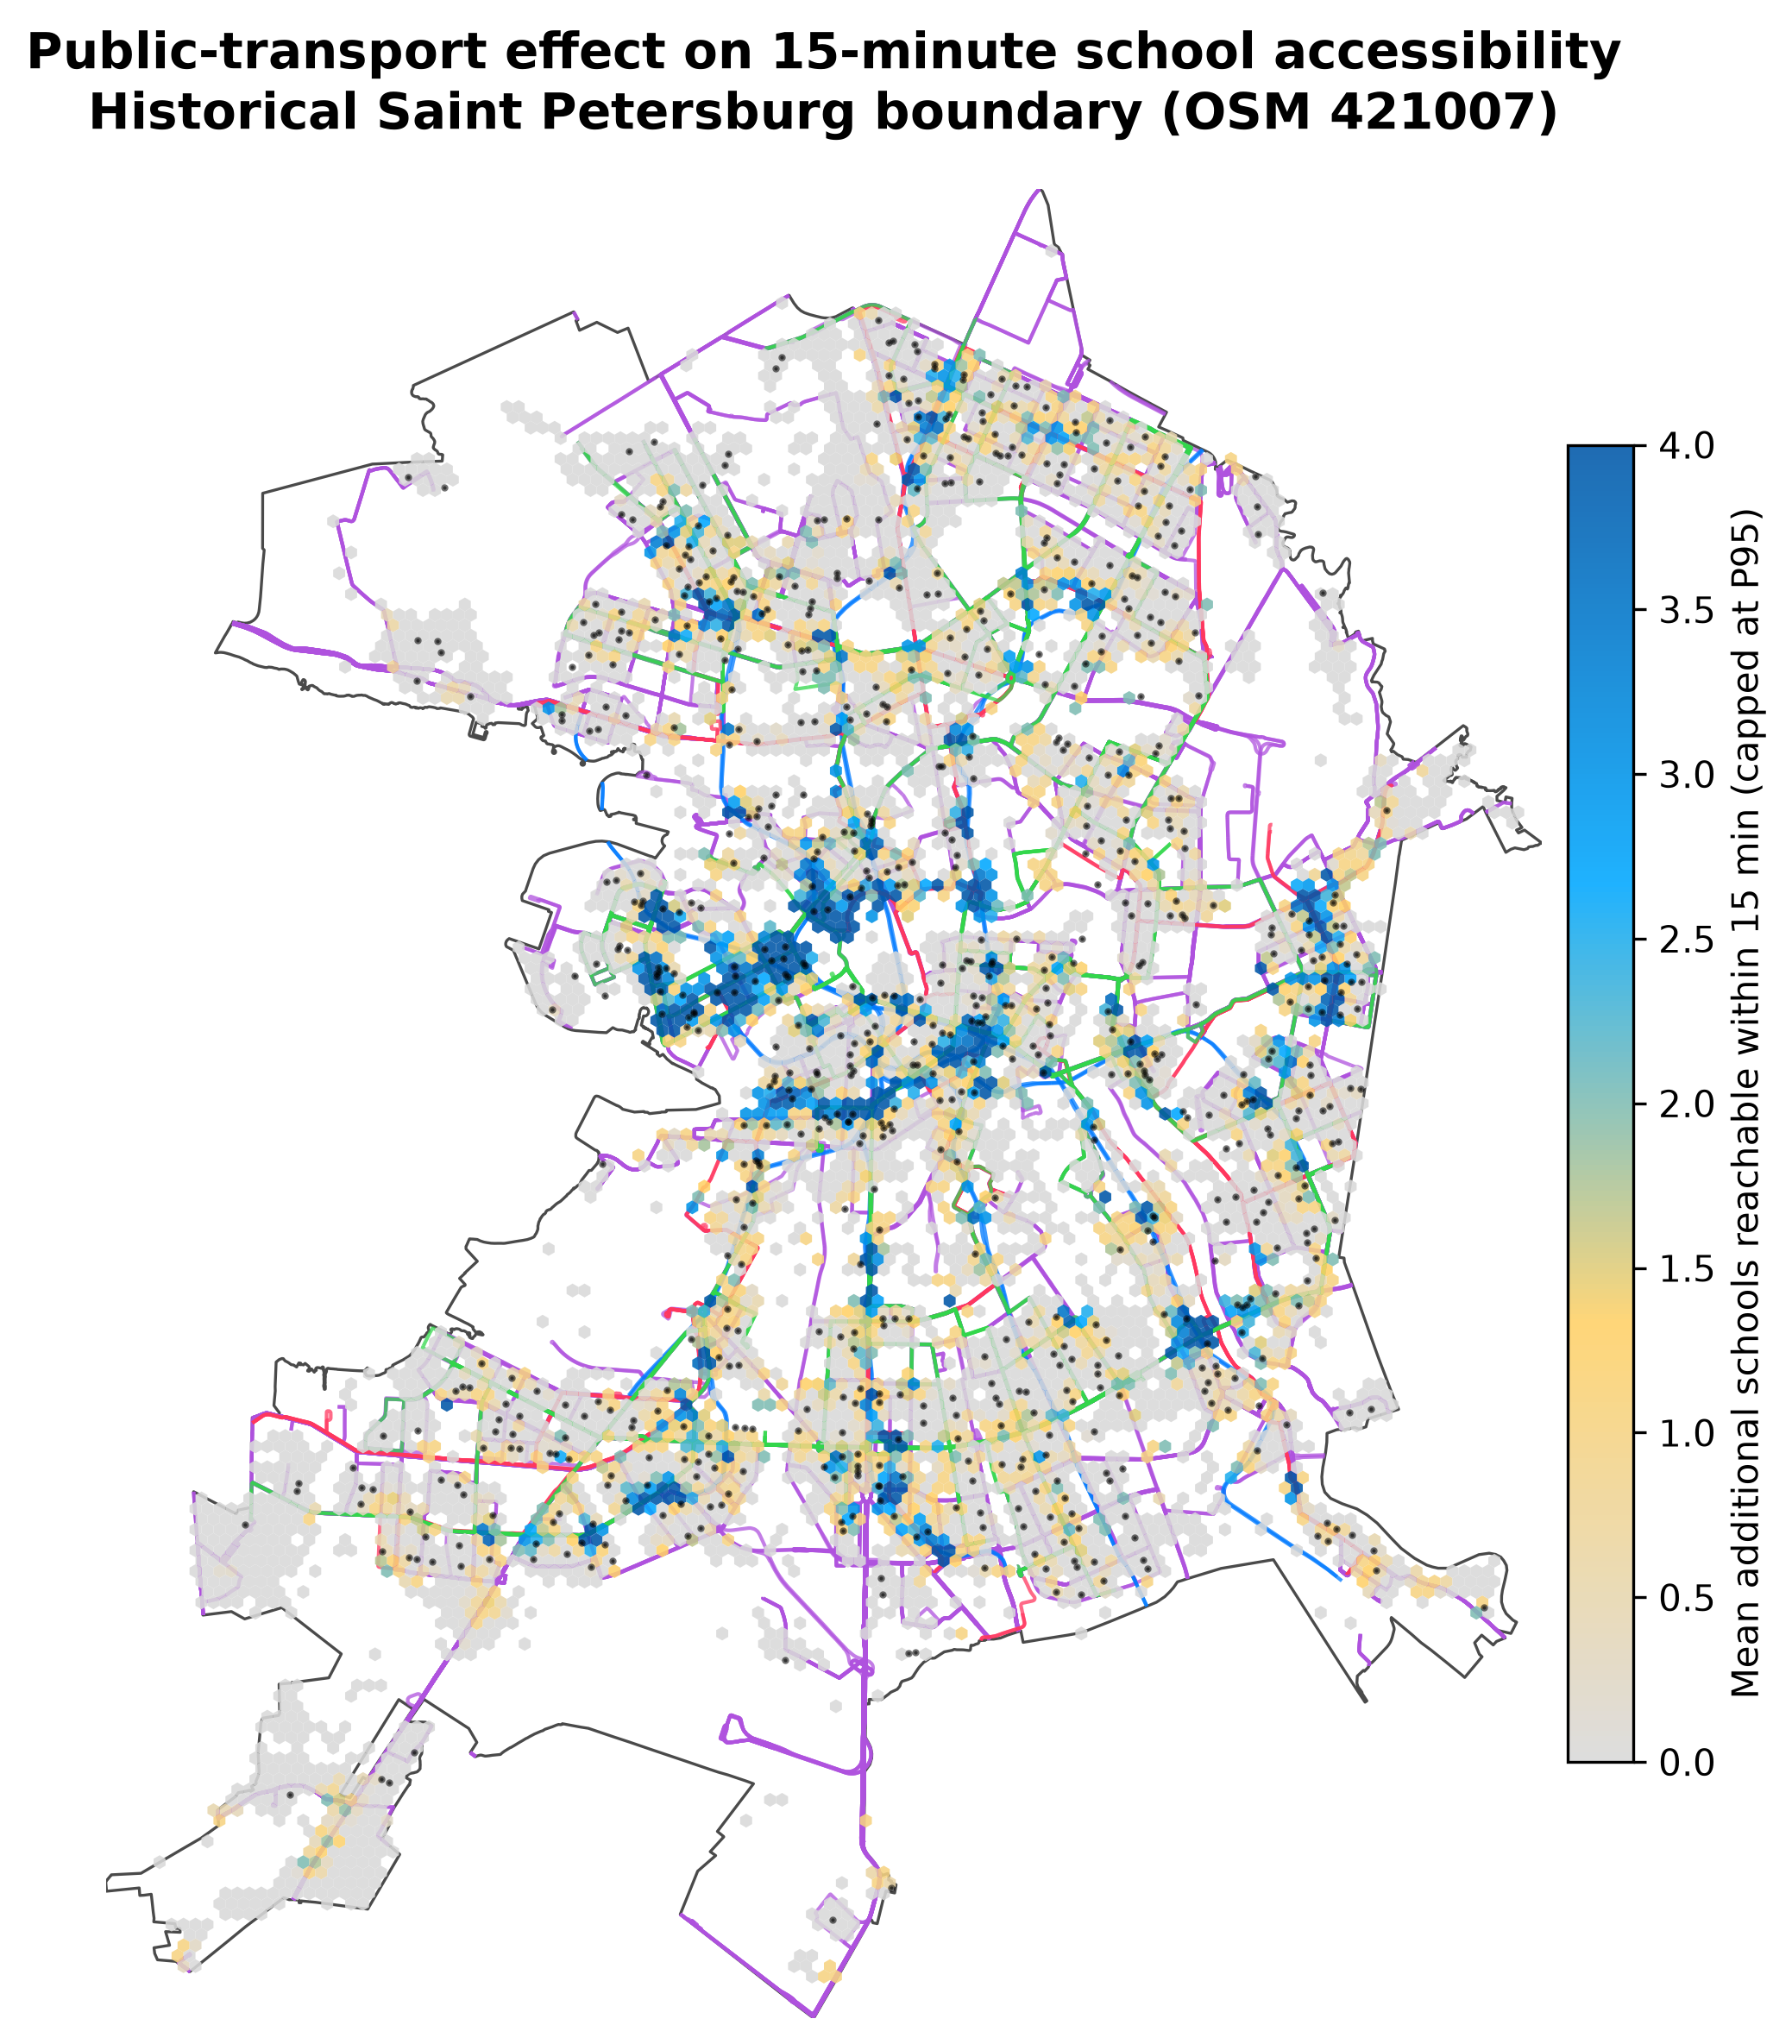
\includegraphics[width=0.6\textwidth]{figures/accessibility_gain_map}
        \caption{Mean additional schools reachable within 15 min per hexagonal cell (capped at the 95th
        percentile), with PT routes and schools (dots) overlaid; historical city boundary.
        Gains concentrate along tram and subway corridors, while large residential areas show no 15-min
        effect.\label{fig:gain_map}}
    \end{figure}

% NB: label suffixes -p1/-p0 are historical (screening was P1, degradation P0 in the
% experiment scripts and released artifacts); the reading order is screening first.
    \subsection{Scenario Screening: Leave-One-Route-Out Route Criticality}
    \label{subsec:res-p1}

    The leave-one-route-out screening covers all 635 PT routes of the city.
    A complete scenario pass takes 6.7~s at the median, and the summed per-route wall-clock time for the
    full screening is 87.0~min on the workstation, fast enough to repeat after any network edit.
    The overall ranking is dominated by the metro (Figure~\ref{fig:p1_ranking} shows the three most
    critical routes of each mode): five metro lines occupy the top five positions, with
    247{,}083, 208{,}837, 167{,}438, 104{,}880 and 86{,}325 lost 30-min opportunities respectively,
    the busiest an order of magnitude above the most critical surface routes (tram 16: 23{,}473; tram
    T1: 16{,}983; bus 211\cyr{Э}: 8{,}485), while trolleybus losses stay in the hundreds.
    Removing metro line 1 alone affects 12{,}893 buildings (15.4\% of origins), with a mean loss of
    3.0 and a maximum of 253 schools per building; even then, no building loses its last 30-min school
    (33 lose their last 15-min school).
    Conversely, most surface routes can be removed with little structural loss for school access; the
    network's redundancy lies mainly in the dense bus layer. A small set of peripheral services is an
    important exception: removing bus 691\cyr{Э}, 211\cyr{Э}, 679 or 211 leaves 216, 212, 143 or 138
    origins, respectively, without any 30-min school, while removing metro line~5 does so for 39 origins.
    Figure~\ref{fig:p1_maps} maps the spatial loss footprints of the most critical route of each
    surface mode alongside metro line 1.
    These results rank \emph{structural} criticality for school opportunities only; they say nothing
    about ridership, capacity or other destinations.

    \begin{figure}[H]
        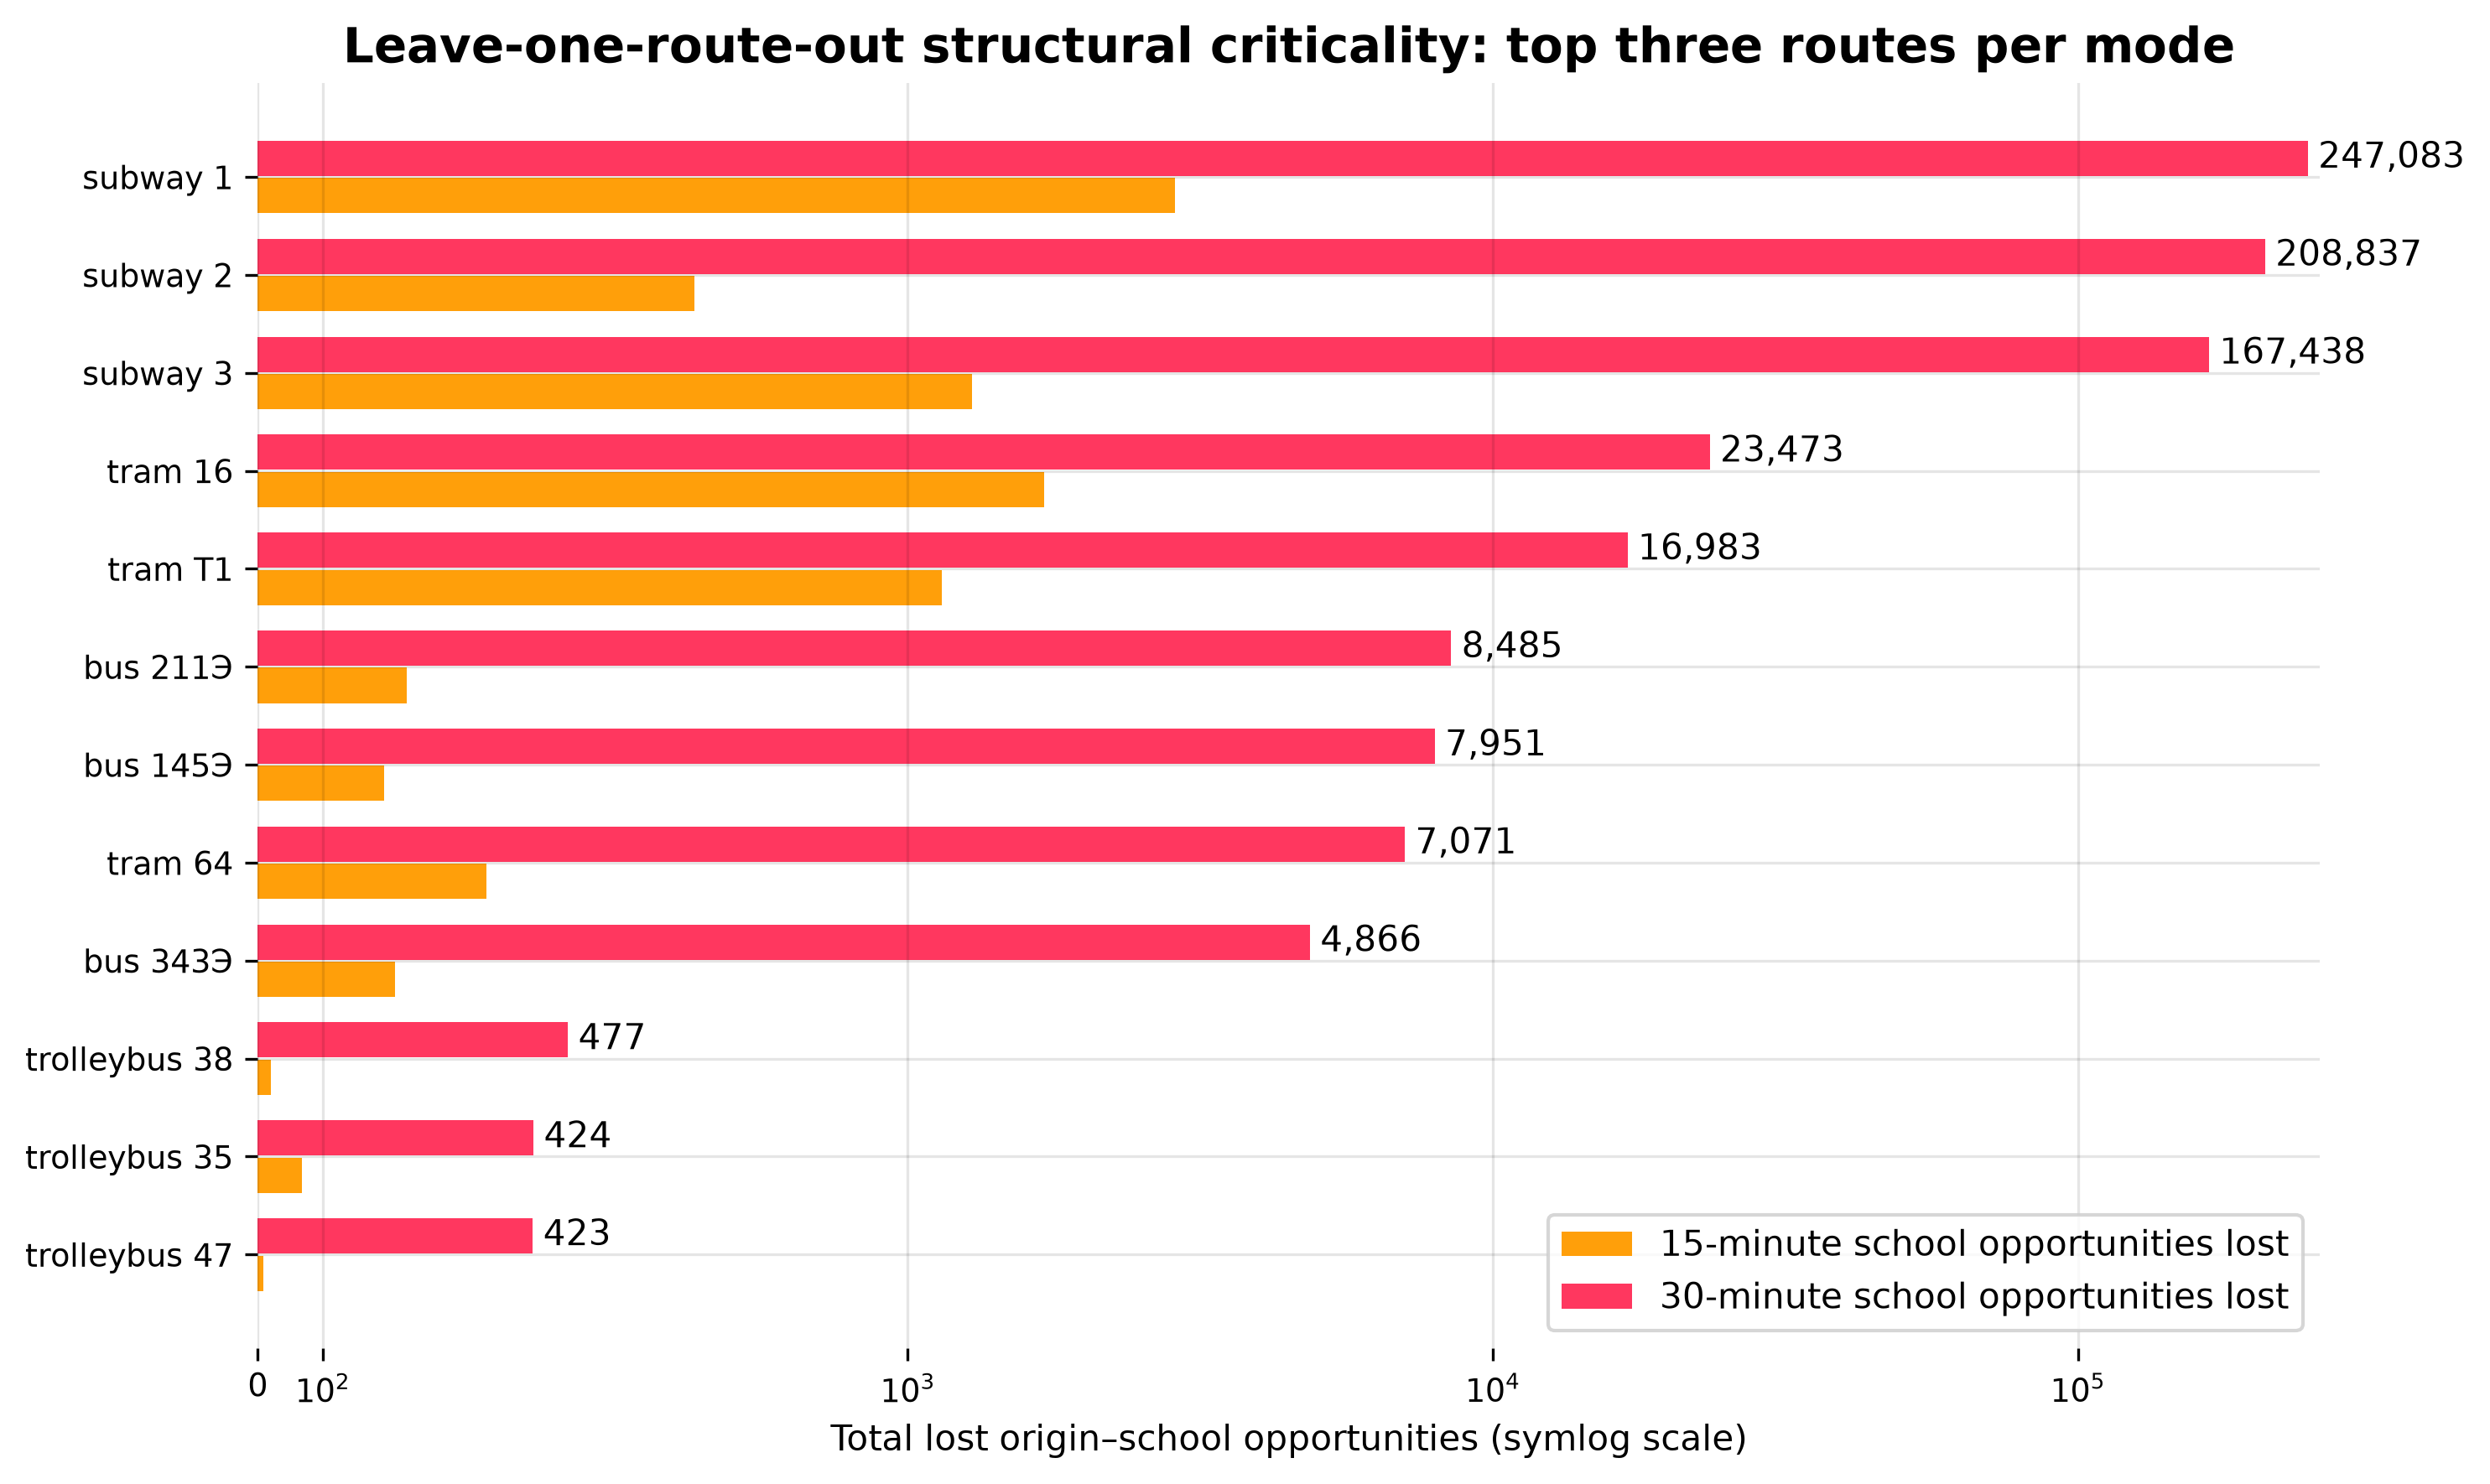
\includegraphics[width=\textwidth]{figures/route_criticality_ranking}
        \caption{Leave-one-route-out criticality: top three routes per mode by lost 15- and 30-min
        origin--school opportunities (symlog scale).\label{fig:p1_ranking}}
    \end{figure}

    \begin{figure}[H]
        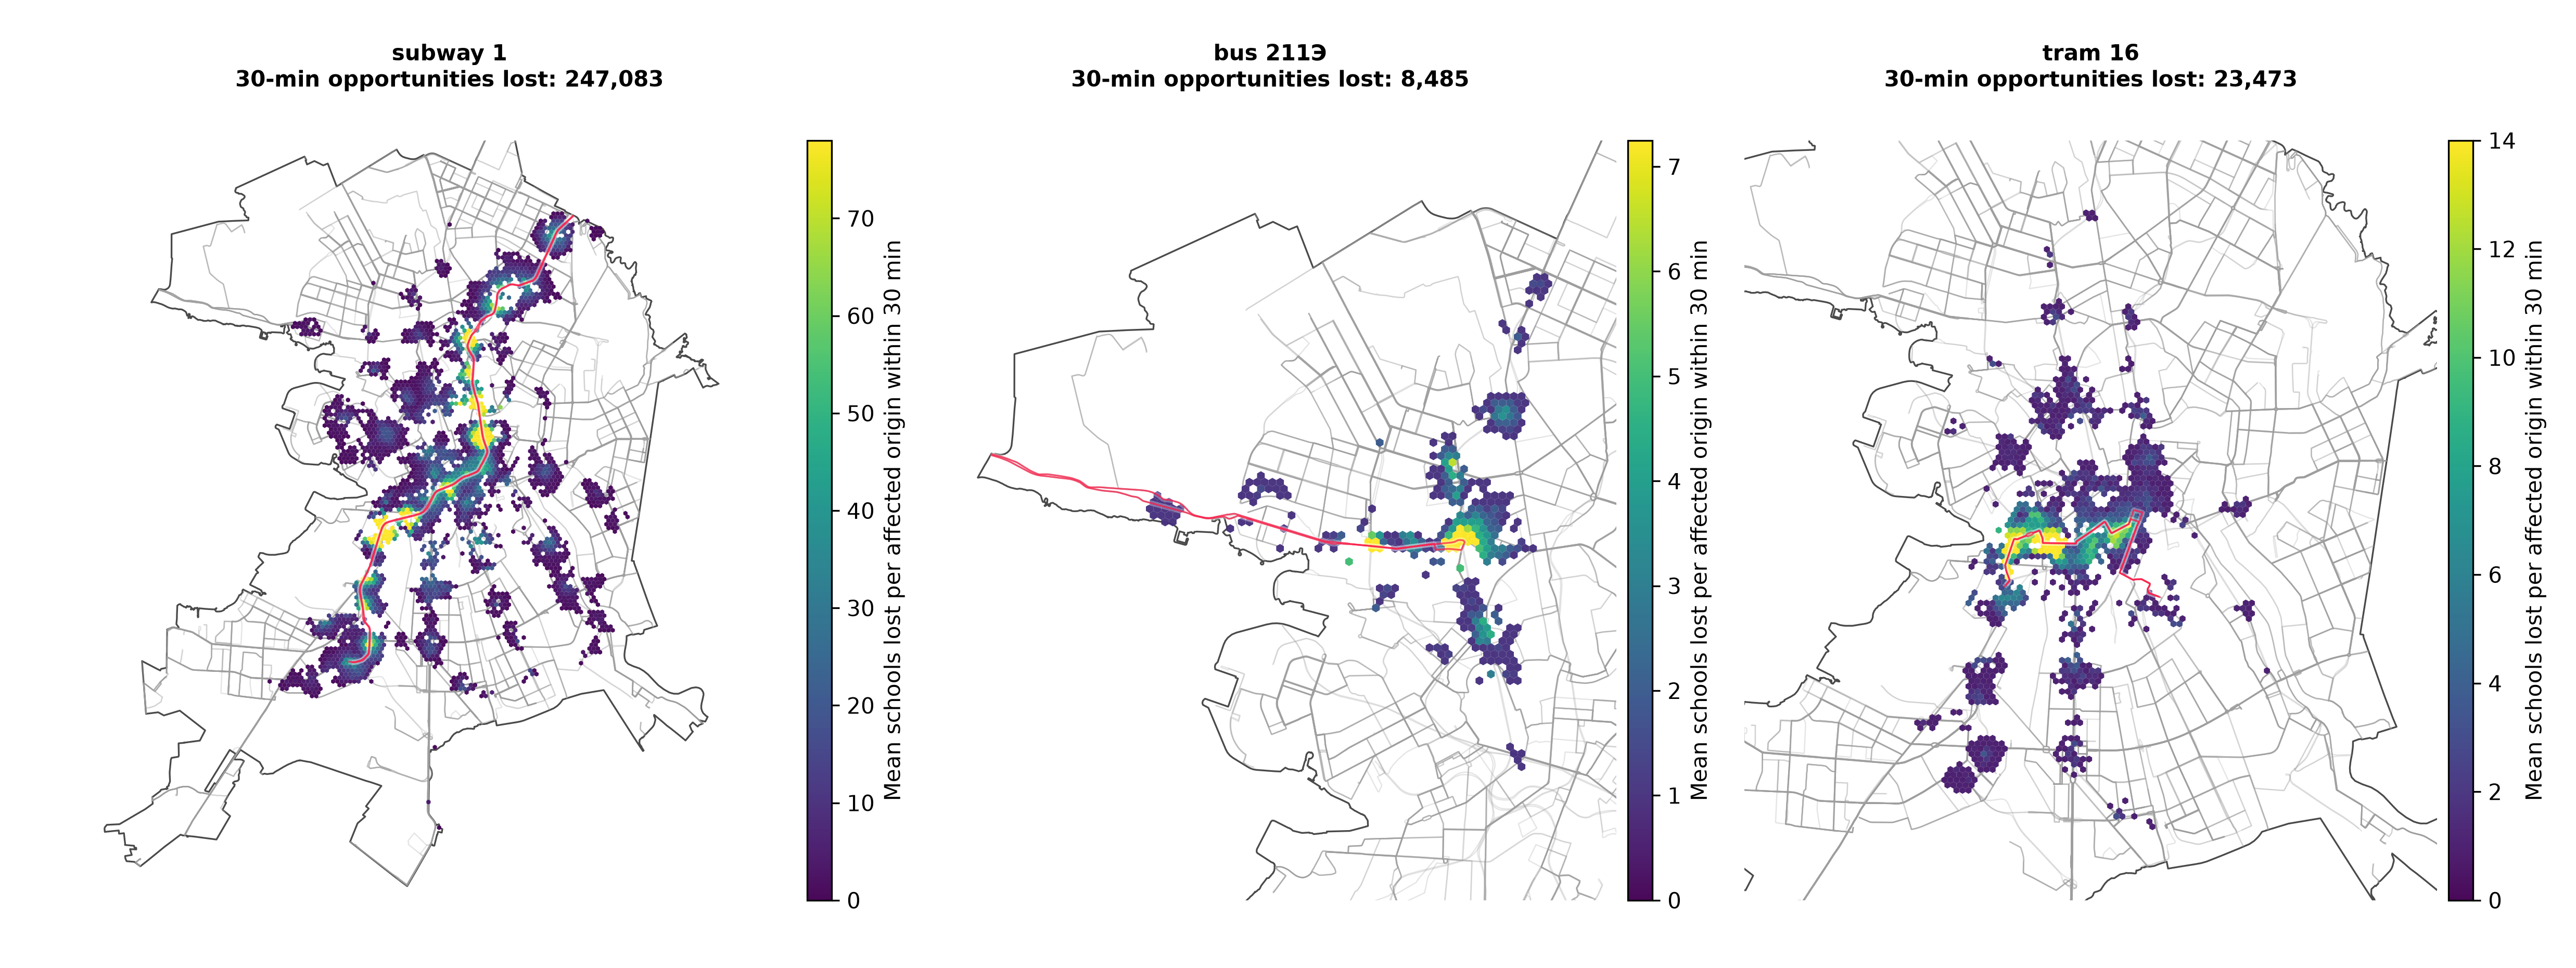
\includegraphics[width=\textwidth]{figures/scenario_p1_top_routes}
        \caption{Spatial loss footprints for the most critical routes (metro line 1, bus
        211\cyr{Э}, tram 16): mean schools lost per affected origin within 30 min;
        the removed route is highlighted. Because route effects differ by an order of magnitude, each
        panel has its own color bar capped at its 95th percentile.\label{fig:p1_maps}}
    \end{figure}

    \subsection{Scenario Analysis: Waiting-Time Degradation}
    \label{subsec:res-p0}

    The degradation experiment targets the tram network: the whole mode, and route~16, which the
    screening above identifies as the structurally most critical tram route---a data-driven choice
    rather than a prior hypothesis.
    Waiting penalties of $+5$ and $+10$~min are added to boarding edges (1{,}823 edges for the mode,
    55 for the route), and all baseline indicators are re-computed; each scenario evaluation takes
    6.3--7.2~s end-to-end.
    Table~\ref{tab:p0} summarizes the losses.
    A uniform $+10$~min penalty on the whole tram mode strips 168{,}504 30-min origin--school
    opportunities (8.6\% of the multimodal baseline total) from 20{,}358 buildings; route~16 alone
    accounts for 23{,}355 opportunities (1.2\%) across 4{,}908 buildings.
    Notably, service degradation almost never severs access altogether: even the mode-wide $+10$~min
    scenario leaves only 42 buildings without their last 30-min school, and the single-route scenarios
    none---waiting quality narrows school choice rather than eliminating it
    (Figure~\ref{fig:p0_delta}).

    \begin{table}[H]
        \caption{Waiting-time degradation ($+5$/$+10$ min on boarding edges): buildings losing at least
        one reachable school and total lost origin--school opportunities at the 15- and 30-min
        cutoffs.\label{tab:p0}}
        \begin{tabularx}{\textwidth}{lCCCC}
            \toprule
            \textbf{Scenario}  & \textbf{Origins (15)} & \textbf{Lost pairs (15)} & \textbf{Origins (30)} & \textbf{Lost pairs (30)}\\
            \midrule
            All trams, +5 min  & 4{,}842               & 11{,}563                 & 20{,}244              & 143{,}570                \\
            All trams, +10 min & 4{,}851               & 11{,}892                 & 20{,}358              & 168{,}504                \\
            Tram 16, +5 min    & 806                   & 1{,}641                  & 4{,}835               & 20{,}354                 \\
            Tram 16, +10 min   & 809                   & 1{,}703                  & 4{,}908               & 23{,}355                 \\
            \bottomrule
        \end{tabularx}
    \end{table}

    \begin{figure}[H]
        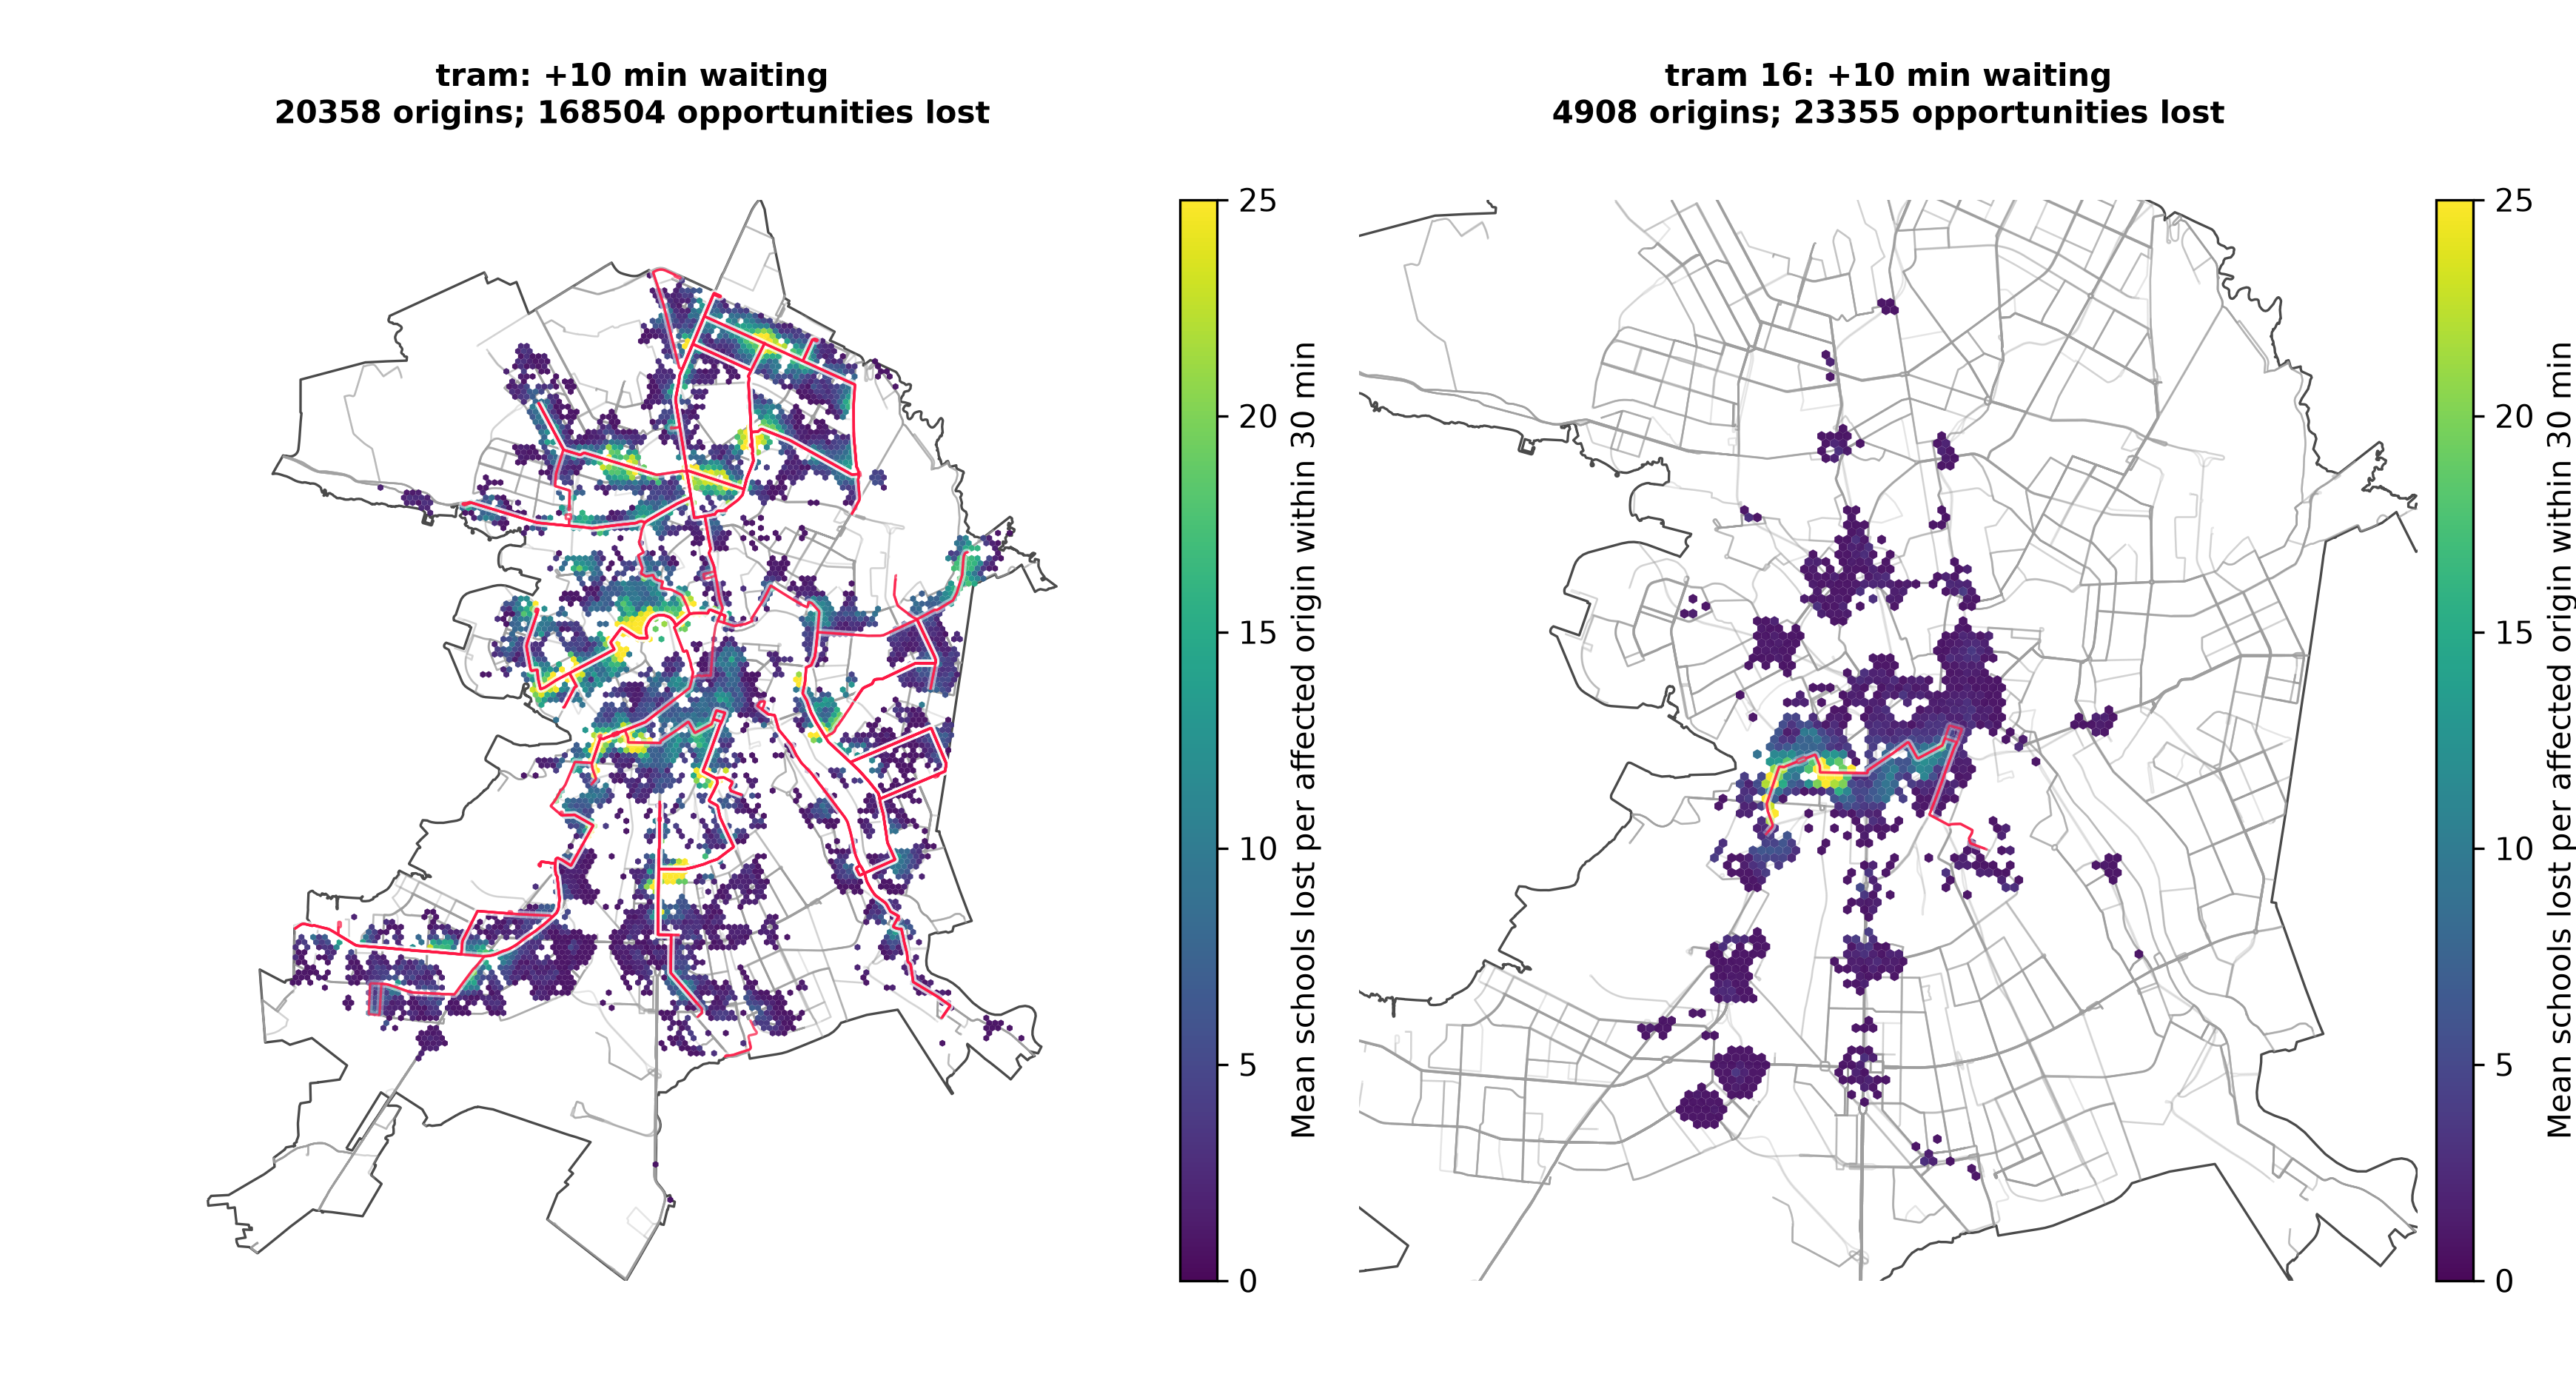
\includegraphics[width=\textwidth]{figures/scenario_p0_waiting_delta}
        \caption{Waiting-time degradation ($+10$ min): mean schools lost per affected origin within 30 min
        for the whole tram mode (\textbf{left}) and for route 16 alone (\textbf{right}); the degraded
        routes are highlighted. Both panels use a common 0--25-school color scale, capped just above the
        larger panel's 95th percentile.\label{fig:p0_delta}}
    \end{figure}

%%%%%%%%%%%%%%%%%%%%%%%%%%%%%%%%%%%%%%%%%%


    \section{Discussion}
    \label{sec:discussion}

    \subsection{Implications for Urban Planning}
    \label{subsec:disc-planning}

    Three planning-relevant readings follow from the case study.
    First, basic school access in Saint Petersburg is walk-dominated: adding PT leaves the median
    nearest-school time unchanged, so policies aimed at first access---school siting, safe walking
    routes---operate on the walk network.
    What PT governs is school \emph{choice}: at a 30-min budget it multiplies the mean opportunity set
    by 2.5, and the gain map shows precisely which corridors deliver this effect and which large
    residential areas receive none.
    Second, the network's critical backbone is thin: the five main metro lines occupy the top five
    criticality ranks and the busiest sits an order of magnitude above any surface route, while most
    of the 635 routes can be removed with little structural loss for school accessibility---redundancy
    that planners can read as robustness of the surface network, with the explicit caveat that our
    metric ignores demand, capacity and destinations other
    than schools.
    Third, service quality matters at scale: a uniform $+10$-min waiting penalty on trams alone strips
    168 thousand 30-min school opportunities from 20 thousand buildings.
    Because each what-if evaluation costs ${\approx}7$~s, such screening can serve as a triage step
    that selects and prioritizes candidate interventions before heavier timetable-aware or behavioral
    modeling is invested in them.

    \subsection{Complementarity with Existing Frameworks}
    \label{subsec:disc-complementarity}

    IduEdu complements rather than replaces existing systems.
    The Mobility Oracle~\cite{gogousou2026mobilityoracle} contributes behavioral approximation of
    mobility; MATSim-based frameworks~\cite{shulajkovska2024framework} contribute agent-based
    simulation; OSRM and OpenTripPlanner~\cite{osrm,otp} contribute low-latency, timetable-aware query
    serving; accessibility platforms~\cite{gumina2026mapping} contribute indicator publication.
    What these systems have in common is a need for an explicit, editable network substrate and cheap
    batch computation---exactly the layer IduEdu provides as an open GeoDataFrame-native graph with fast
    routing primitives.
    A behavioral or simulation model can define its own edge costs, mode preferences and network
    modifications over \texttt{UrbanGraph} tables and re-use the computational kernels, instead of
    maintaining a private graph format and conversion pipeline.

    \subsection{Transferability and Computational Accessibility}
    \label{subsec:disc-transferability}

    The pipeline is deliberately OSM-only: it requires neither GTFS feeds, nor smart-card records, nor
    surveys, nor a deployed routing service.
    This lowers the entry cost for research groups and municipal teams in data-constrained cities,
    where such data are unavailable or stale.
    All experiments in this paper ran on a single workstation; the full city-scale case study,
    including scenario screening, is reproducible without cluster infrastructure.
    The construction benchmarks cover six cities of varying scale and structure, supporting
    transferability of the graph-building stage; the applied case study itself is demonstrated for one
    city, and its urban conclusions should be transferred with the usual caution.

    \subsection{Extensibility and Downstream Applications}
    \label{subsec:disc-extensibility}

    Applications already realized by the IduEdu + ObjectNat pair include education and healthcare
    accessibility audits; single- and multi-origin (stepped) isochrones; graph-based catchment and
    coverage zones for service sets; nearest-service assignment with identification of uncovered areas;
    and capacity-aware service provision where demand and capacity data exist.
    Applications that are possible but require an additional domain model include underserved-zone
    detection, rapid screening of route or station closures and candidate interventions, structural
    resilience assessment, serving as a backend for urban digital twins and scenario dashboards,
    behavioral simulation of mode and route choice, and preparation of features and matrices for
    demand, land-use and equity models.
    The distinction matters: the former are demonstrated capabilities, the latter are extensibility
    claims supported by the architecture but not yet by experiments.

    \subsection{Limitations}
    \label{subsec:disc-limitations}

    Several limitations bound the interpretation of our results.
    The PT model is static: it encodes route topology and modeled travel times, without timetables,
    congestion, demand or passenger behavior; user-defined waiting penalties are scenario parameters,
    not recovered schedules.
    This is a limitation of the paper's experimental coverage, not of the public API's scenario
    surface.
    Graph quality depends directly on OSM completeness and correctness for the studied territory.
    The routing benchmark uses one city's multimodal graph and one workstation; construction benchmarks
    span six cities, but hardware diversity was not studied.
    The accessibility results quantify \emph{structural} accessibility of residential locations under
    modeled travel times, not experienced door-to-door times, and---beyond the secondary
    population-weighted coverage figures---must not be read as social equity measures.

    Several threats to validity deserve explicit note.
    OSM completeness for PT routes and school locations varies across cities and time; our network
    reflects a July 2026 snapshot. The route-count comparison against the city register
    (Table~\ref{tab:pt_validity}) agrees closely for electric modes and exactly for the metro but
    overcounts buses by ${\approx}20\%$, consistently with heterogeneous OSM route variants and the
    analysis buffer.
    The per-mode speed models, the 1-min boarding cost and the scenario waiting penalties are
    assumptions: conclusions about absolute travel times are correspondingly softer than the relative
    walk-vs-multimodal and baseline-vs-scenario comparisons, which share the same assumptions on both
    sides.
    The residential filter (83{,}510 of 168{,}886 footprints) and the modeled balanced allocation of
    population to buildings bound the interpretation of the population-weighted coverage difference.
    Finally, all reported timings exclude JIT warm-up, which a cold process pays once
    (${\approx}17$~s on the first scenario), and were obtained on a single workstation.

%%%%%%%%%%%%%%%%%%%%%%%%%%%%%%%%%%%%%%%%%%


    \section{Conclusions}
    \label{sec:conclusions}

    This paper presented IduEdu, an open-source GeoDataFrame-native pipeline for constructing
    multimodal urban graphs from OpenStreetMap and computing accessibility at city scale.
    Returning to the research questions: (RQ1) a single OSM-based pipeline does construct a correct,
    explicit and compact multimodal representation without GTFS---reachability matches a NetworkX
    reference exactly, travel times agree within $3\cdot10^{-4}$~min, and network length matches OSMnx
    within ${\approx}1\%$; (RQ2) the unified tabular representation reduces street-graph construction
    time $3.3$--$9.3\times$ relative to OSMnx (median ${\approx}8.8\times$ without simplification,
    ${\approx}5.7\times$ with it) with an order-of-magnitude smaller in-memory footprint, and removes
    the conversion step that specialized graph backends require;
    (RQ3) adaptive reversal and cutoff make batch OD workloads scale to $10^5$ origins on a
    workstation, and a cached baseline graph turns a full city-scale scenario re-evaluation into a
    ${\approx}7$-second operation---all 635 PT routes of Saint Petersburg were screened in 87~min;
    (RQ4) the multimodal layer changes the assessment substantially, but not where one might expect: a
    walk-only analysis characterizes basic access correctly---the median nearest-school time is
    unchanged---yet understates the reachable opportunity set 2.5-fold at a 30-min budget and cannot
    reveal that this set rests on a thin backbone, with the five main metro lines taking the top five
    criticality ranks, an order of magnitude above any surface route; the effect is also spatially
    uneven, half of the residential buildings seeing no 15-min gain.

    The technical takeaway is that the user-facing and computational forms of an urban network need not
    be separate artifacts: making the GIS table canonical and deriving the sparse computational view
    lazily preserves the familiar GeoPandas workflow while matching optimized backends on batch
    workloads.
    The urban takeaway is that, for school accessibility in Saint Petersburg, public transport acts as
    an amplifier of choice rather than a provider of basic access, and that this choice rests on a
    small critical backbone---a diagnosis the presented pipeline can reproduce for any other
    OSM-covered city in minutes.
    The approach is bounded by its static, structural notion of accessibility: extending it with GTFS
    and time-dependent routing would broaden structural analysis to service-aware accessibility, and
    remains future work.
    GTFS integration need not require time-dependent routing: it could first supply schedule-derived travel
    and waiting costs to the existing static \texttt{UrbanGraph}.

    Within that boundary, IduEdu offers a reproducible, low-cost foundation for smart-mobility
    analytics in cities where data are scarce but planning questions are not.

%%%%%%%%%%%%%%%%%%%%%%%%%%%%%%%%%%%%%%%%%%
    \vspace{6pt}

    \authorcontributions{Conceptualization, methodology, software, validation, formal analysis,
        investigation, data curation, writing---original draft preparation, visualization: D.O.;
        supervision, writing---review and editing: N.C.
        All authors have read and agreed to the published version of the manuscript.}

    \funding{This research was carried out with the financial support of the Foundation for Support
        of Projects of the National Technology Initiative within the framework of the roadmap for the
        development of the high-technology area ``Artificial Intelligence'' for the period until 2030,
        agreement No.~70-2021-00187.}

    \institutionalreview{Not applicable.}

    \informedconsent{Not applicable.}

    \dataavailability{The IduEdu source code and reproducibility scripts are available at
    \url{https://github.com/DDonnyy/IduEdu}. The OSM-derived inputs, processed benchmark outputs,
        graph snapshots, environment manifests and case-study artifacts used in this study are openly
        available in Zenodo at \url{https://doi.org/10.5281/zenodo.21610964}. OpenStreetMap data are
        available under the Open Database License from \url{https://www.openstreetmap.org}.}

    \acknowledgments{During preparation of this manuscript, the authors used OpenAI GPT-5 and Claude Opus 4.8
    for language editing, consistency checks, code-assisted verification against the reported artifacts,
        and implementation of benchmark and comparative-figure generation scripts. The benchmark protocols,
        comparison criteria, metrics, and figure concepts and specifications were designed by the authors; the
        AI systems assisted in translating those designs into executable code. The authors reviewed, tested,
        and edited all AI-assisted code and text and take full responsibility for the analysis, results, and
        content of the publication.
    }

    \conflictsofinterest{The authors declare no conflicts of interest.}

    \abbreviations{Abbreviations}{%
        The following abbreviations are used in this manuscript:\\

        \noindent
        \begin{tabular}{@{}ll}
            OSM  & OpenStreetMap                      \\
            OD   & Origin--Destination                \\
            PT   & Public Transport                   \\
            GTFS & General Transit Feed Specification \\
            CSR  & Compressed Sparse Row              \\
            AOI  & Area of Interest                   \\
            JIT  & Just-in-Time (compilation)         \\
            KPI  & Key Performance Indicator          \\
        \end{tabular}
    }

%%%%%%%%%%%%%%%%%%%%%%%%%%%%%%%%%%%%%%%%%%
    \appendixtitles{yes}
    \appendixstart
    \appendix


    \section{Sensitivity of the Spatial Effect Classification}
    \label{app:class-sensitivity}

    Table~\ref{tab:class-sensitivity} varies the absolute and relative thresholds used to distinguish
    \emph{moderate} from \emph{substantial} opportunity gains at the 15-min reference cutoff. The shares of
    the no-effect (48.58\%), newly reachable (2.47\%) and unreachable (33.70\%) classes do not depend on
    these two thresholds. Across the tested grid, the substantive result is stable: most origins either
    show no 15-min effect or remain unreachable, while the combined moderate and substantial share stays
    at 15.26\%. The relative threshold drives the split within that positive-gain group; changing the
    absolute threshold from 5 to 15 schools has a negligible effect.

    \begin{table}[H]
        \caption{Sensitivity of the 15-min spatial effect classification. The bold row is the specification
        used in the main analysis. Shares are percentages of all 83{,}510 residential origins.
        \label{tab:class-sensitivity}}
        \centering
        \begin{tabularx}{0.72\textwidth}{CCCC}
            \toprule
            \textbf{$\gamma_{\mathrm{abs}}$ (schools)} &
            \textbf{$\gamma_{\mathrm{rel}}$ (\%)} &
            \textbf{Moderate (\%)} &
            \textbf{Substantial (\%)}\\
            \midrule
            5          & 10          & 0.91          & 14.34         \\
            5          & 20          & 4.16          & 11.10         \\
            \textbf{5} & \textbf{25} & \textbf{5.58} & \textbf{9.68} \\
            5          & 30          & 7.33          & 7.93          \\
            10         & 10          & 0.91          & 14.34         \\
            10         & 20          & 4.16          & 11.10         \\
            10         & 25          & 5.58          & 9.68          \\
            10         & 30          & 7.34          & 7.92          \\
            15         & 10          & 0.91          & 14.34         \\
            15         & 20          & 4.16          & 11.10         \\
            15         & 25          & 5.58          & 9.68          \\
            15         & 30          & 7.34          & 7.92          \\
            \bottomrule
        \end{tabularx}
    \end{table}

%%%%%%%%%%%%%%%%%%%%%%%%%%%%%%%%%%%%%%%%%%
    \begin{adjustwidth}{-\extralength}{0cm}

        \reftitle{References}

        \bibliography{sample-base}

        \PublishersNote{}
    \end{adjustwidth}
\end{document}
